\documentclass[11pt,%
%draft,% seulement brouillon
twoside,% twoside si document final
a4paper,%
openright % openright si document final
]{book}

%\usepackage{cmbright} % fichier + lisible sur ordi, - lisible sur papier
\usepackage[utf8]{inputenc} %gestion des accents par le compilateurs
\usepackage[cyr]{aeguill}
\usepackage[T1]{fontenc} %gestion des accents par l'afficheurs et la césure
\usepackage[french]{babel} % traduction des packages

\usepackage{lmodern} % fontes tailles variables
% substitution des petites capitales grasses manquantes
\rmfamily
\DeclareFontShape{T1}{lmr}{b}{sc}{<->ssub*cmr/bx/sc}{}
\DeclareFontShape{T1}{lmr}{bx}{sc}{<->ssub*cmr/bx/sc}{}

\usepackage{tabularx} % Permet d'utiliser l'environnement tabularx
\usepackage{graphicx} % gestion de figure, dessins
\usepackage[dvipsnames]{xcolor} % charge des couleurs

\usepackage{xspace}
\usepackage[%
% paperwidth=270.0mm,%  A supprimer si plus besoin de todonotes
headheight=14pt,%
top    = 2.5cm,%
bottom = 2.5cm,%
%left   = 2cm,%
%right  = 2cm,%
]{geometry} % feuille a4 de taille 21.0 x 29.7 

% suite de paquets mathematiques
\usepackage{amsthm} % gestion des théoremes
\usepackage{amsfonts} % gestions des polices mathématques
\usepackage{amsmath}

\usepackage[autostyle=true]{csquotes}
\usepackage[%
  language=english,%
  sorting=ynt,%
  backend=biber,%
  style=alphabetic,%
  hyperref=true,%
  giveninits=true, % initialles pour prénoms
  isbn=false,%
  url=false,%
  doi=false,%
  backref=true,%
  backrefstyle=three% si cité en page 1,2,3, ecrire 1-3, 
  ]{biblatex}
  \renewbibmacro{in:}{} 
  \DeclareFieldFormat[book,report]{title}{\mkbibquote{#1\isdot}}
  \DefineBibliographyStrings{french}{%
    bibliography = {Références},
  }
\usepackage[%
  linkcolor=blue!70!black,%
  colorlinks=true,%
  citecolor=purple%
  ]{hyperref} % gestion des liens hypertexts et reférences

\usepackage{excludeonly}

\usepackage[section]{placeins} % Place un FloatBarrier à chaque nouvelle section
\usepackage{epigraph}
\usepackage[francais,nohints]{minitoc}   % Mini table des matières, en français
\setcounter{minitocdepth}{2} % Mini-toc détaillées (sections/sous-sections)
\usepackage[Lenny]{fncychap}

%\usepackage{multicol} % texte sur plusieurs colonnes
%\usepackage{wrapfig} % permet de gérer les flotants dans les multiples colonnes

\usepackage[%
acronym,%
nomain,%
sanitizesort=false,%
style=super4col%
]{glossaries} %voir glossaire.tex

\setcounter{tocdepth}{1} % Sommaires n'inclus que les niveau 1 à 2 : section, sous-section
\setlength\parindent{0pt} % pas d'alinéa à chaque paragraphe

\usepackage{tikz} % Permet de tracer des figures et schémas
\usetikzlibrary{calc} % permet de réaliser des calculs dans tikz

% \setlength{\oddsidemargin}{25mm}
% \setlength{\evensidemargin}{25mm}
% \setlength{\textwidth}{170mm} 
% \reversemarginpar
% \usepackage{todonotes} % permet d'ajouter des notes en marges

\usepackage{fancyhdr}      % Entête et pieds de page. Doit être placé APRES geometry
  \pagestyle{fancy}    % Indique que le style de la page sera justement fancy
  \fancyfoot[CE,CO]{}
  \fancyfoot[LE,RO]{\thepage}
  \fancyhead[RE,LO]{}
  \fancyhead[RO]{\tiny{\rightmark}}
  \fancyhead[LE]{\tiny{\leftmark}}
%\bibliographystyle{apalike}

\usepackage{array}   % for \newcolumntype macro
\usepackage{multirow}
\newcolumntype{L}{>{$}l<{$}} % math-mode version of column type
\newcolumntype{C}{>{$}c<{$}}
\newcolumntype{R}{>{$}r<{$}}

\usepackage{tcolorbox}
\bibliography{bib/Zotero}
%redefinition
\renewcommand{\frac}[2]{\dfrac{#1}{#2}} % Toujours de grandes fractions
\renewcommand{\tilde}[1]{\overset{\thicksim}{#1}} % Toujours un grand tilde
\newcommand{\tagit}{\addtocounter{equation}{1}\tag{\theequation}}
\newcommand{\ds}{\displaystyle}

\newcommand{\secref}[1]{(\S \ref{#1})}

\newcommand{\CSU}[2][{}]{\ensuremath{\operatorname{CSU}_{\operatorname{#2}}^{#1}}}

% Notation produit vectoriel
\newcommand{\pvect}{\wedge}

% Notation vectorielle
\newcommand{\comp}[1]{{\underline{#1}}} % {\overset{\rightarrow{}}{#1}}

%\newcommand{\vect}[1]{\vec{#1}}
\newcommand{\vect}[1]{{\overset{\rightarrow}{#1}}}

% Notation matricielle
\newcommand{\mat}[1]{\mathbf{#1}}

% Le conjugé
% \newcommand{\conj}[1]{{{#1}^*}}
\newcommand{\conj}[1]{{\overline{#1}}}

\newcommand{\ps}[2]{\left<{#1},{#2}\right>}
\newcommand{\norm}[1]{\left\lVert#1\right\rVert}

% Quelques matrices qui reviennent
\newcommand{\mI}{\mat{I}}
\newcommand{\mZ}{\mat{Z}}
\newcommand{\mA}{\mat{A}}
\newcommand{\mB}{\mat{B}}
\newcommand{\mPP}{\mat{P}}
\newcommand{\mC}{\mat{C}}
\newcommand{\mM}{\mat{M}}
\newcommand{\mJ}{\mat{J}}
\newcommand{\mj}{\mat{j}}
\newcommand{\mH}{\mat{H}}
\newcommand{\mh}{\mat{h}}
\newcommand{\mN}{\mat{N}}
\newcommand{\mMt}{\mat{\tilde{M}}}
\newcommand{\mNt}{\mat{\tilde{N}}}
\newcommand{\mLD}{\mat{L_D}}
\newcommand{\mLR}{\mat{L_R}}
\newcommand{\mL}{\mat{L}}
\newcommand{\mR}{\mat{R}}
\newcommand{\mT}{\mat{T}}
\newcommand{\mF}{\mat{F}}
%\newcommand{\mPt}{\mat{\tilde{P}}}
%\newcommand{\mP}{\mat{P}}
\newcommand{\mS}{\mat{S}}
\newcommand{\mSt}{\mat{\tilde{S}}}

% Matrices de Gramm de la base #1 vers #2
\newcommand{\mG}[2]{\mat{G}^{#1#2}}

% Matrices de passage de la base #1 vers #2 projeté sur #3
\newcommand{\mP}[3]{{\overset{#3}{\underset{#1 \rightarrow #2}{\mat{P}}}}}

% Opérateur pseudo diff
\newcommand{\Op}[2]{{\operatorname{Op}\left(#1\right)\left(#2\right)}}

\newcommand{\w}{\omega}

%mathematical symbol
\newcommand{\RR}{\mathbb R}
\newcommand{\CC}{\mathbb C}
\newcommand{\NN}{\mathbb N}
\newcommand{\ZZ}{\mathbb Z}
\newcommand{\eps}{\epsilon}
\newcommand{\dd}{\mathrm{d}}
\newcommand{\OO}{\Omega}

\newcommand{\ddp}[3][{}]{\dfrac{\mathrm{d}^{#1}#3}{{\mathrm{d}#2}^{#1}}}
\newcommand{\ddr}[3][{}]{\dfrac{\partial^{#1} #3}{{\partial #2}^{#1}}}

%Operator
\newcommand{\Sobolev}[1][{}]{\mathrm{H}_\mathrm{#1}}
\newcommand{\Hgrad}{\Sobolev[grad]}
\newcommand{\Hrot}{\Sobolev[rot]}
\newcommand{\Hdiv}{\Sobolev[div]}
\newcommand{\Hess}{\operatorname{Hess}}
\renewcommand{\Re}{\operatorname{Re}}
\renewcommand{\Im}{\operatorname{Im}}

\newcommand{\diag}[2]{\operatorname{diag}\left(#1,#2\right)}

\newcommand{\sign}[1]{{\operatorname{sign}\left(#1\right)}}
\newcommand{\argmin}[1]{{\underset{#1}{\operatorname{argmin}}}}
\newcommand{\Ker}{\operatorname{Ker}}
\newcommand{\Img}{\operatorname{Img}}
\newcommand{\Vect}[1]{\operatorname{Vect}\left\lbrace#1\right\rbrace}

\newcommand{\Tr}{\operatorname{T_R}}
\newcommand{\oI}{{\mathcal{I}}}
\newcommand{\LD}{{\mathcal{L}_D}}
\newcommand{\LL}{\mathcal{L}}
\newcommand{\LR}{{\mathcal{L}_R}}

\newcommand{\EFIE}{\operatorname{EFIE}}
\newcommand{\MFIE}{\operatorname{MFIE}}
\newcommand{\CFIE}{\operatorname{CFIE}}

%Maxwell notations
\newcommand{\vE}{\vect{E}}
\newcommand{\vH}{\vect{\mathcal{H}}}
\newcommand{\vn}{\vect{n}}
\newcommand{\vx}{\vect{x}}
\newcommand{\vz}{\vect{z}}
\newcommand{\vy}{\vect{y}}
\newcommand{\vk}{\vect{k}}
\newcommand{\vJ}{\vect{J}}
\newcommand{\vK}{\vect{K}}
\newcommand{\vM}{\vect{M}}
\newcommand{\vA}{\vect{A}}
\newcommand{\vu}{\vect{u}}
\newcommand{\vv}{\vect{v}}
\newcommand{\vw}{\vect{w}}

%differential operator
\newcommand{\vgrad}{\vect{\nabla}}
\newcommand{\vdiv}{\vect{\nabla}\cdot}
\newcommand{\vrot}{\vect{\nabla}\pvect}
\newcommand{\vhess}{\vect{\Hess}}

\newcommand{\tgrad}{{\vect{\operatorname{grad}}}}
\newcommand{\trot}{{\vect{\operatorname{rot}}}}
\newcommand{\tdiv}{{\operatorname{div}}}

\newcommand{\vgrads}{\vect{\nabla_s}}
\newcommand{\vdivs}{\vect{\nabla_s} \cdot}
\newcommand{\vrots}{\vect{\nabla_s} \pvect}
\newcommand{\rots}{{\nabla_s} \pvect}
\newcommand{\vhesss}{\vect{\Hess_s}}

\newcommand{\mhess}{\mat{\Hess}}
\newcommand{\mhesss}{\mat{\Hess}_s}

\newcommand{\tgrads}{{\vect{\operatorname{grad}}_s}}
\newcommand{\trots}{{{\operatorname{rot}}_s}}
\newcommand{\tvrots}{{\vect{\operatorname{rot}}_s}}
\newcommand{\tdivs}{{\operatorname{div}_s}}

\newcommand{\lapl}{\Delta}
\newcommand{\lapls}{\Delta_s}
\newcommand{\vlapl}{\vect{\Delta}}
\newcommand{\vlapls}{\vect{\Delta_s}}

% helmotlz
\newcommand{\rtp}{r,\theta,\phi}
\newcommand{\tp}{\theta,\phi}

\newcommand{\PP}{\mathbb{P}}
\newcommand{\Pmn}{\PP^m_n}

% cioe
\newcommand{\ov}[1]{\overline{#1}}

\newcommand{\x}{{x}}
\newcommand{\y}{{y}}
\newcommand{\z}{{z}}

\newcommand{\kO}{\mathbf{k_0}}
\newcommand{\etaO}{\boldsymbol{\eta_0}}
\newcommand{\muO}{\boldsymbol{\mu_0}}
\newcommand{\epsO}{\boldsymbol{\eps_0}}
\newcommand{\nuO}{\boldsymbol{\nu_0}}

%
\newcommand{\peps}{{\epsilon}}
\newcommand{\pmu}{{\mu}}

\newcommand{\phii}{\vect{\phi_i}}
\newcommand{\pii}{\vect{p_i}}
\newcommand{\phin}{\vect{\phi_n}}
\newcommand{\phim}{\vect{\phi_m}}
\newcommand{\pn}{\vect{p_n}}
\newcommand{\ppm}{\vect{p_m}}
\newcommand{\phip}{\vect{\phi_p}}
\newcommand{\phiq}{\vect{\phi_q}}
\newcommand{\pj}{\vect{p_j}}
\newcommand{\qj}{\vect{q_j}}
\newcommand{\qi}{\vect{q_i}}
\newcommand{\nuj}{\vect{\nu_j}}
\newcommand{\uj}{\vect{u_j}}
\newcommand{\phij}{\vect{\phi_j}}

%% avec référence dans la table des matières et les bons en-têtes
%% il sert pour l'introduction, la page de notations, etc
\newcommand{\chapterstar}[1]{%
  \chapter*{#1}%
  \addcontentsline{toc}{chapter}{#1}%
  %\markboth{#1}{#1}
  }
\newcommand{\sectionstar}[1]{%
  \section*{#1}%
  \addcontentsline{toc}{section}{#1}%
  %\markboth{#1}{#1}
  }

\newcommand{\Mmn}[1][{}]{\vect{M_{m,n}^{#1}}}
\newcommand{\Nmn}[1][{}]{\vect{N_{m,n}^{#1}}}
\newcommand{\Umn}[1][{}]{\vect{U_{m,n}^{#1}}}

\newcommand{\NaN}{\operatorname{NaN}}
\newcommand{\e}[1]{\mathrm{e}{#1}}

\newcommand{\fonction}[5]{
  \begin{aligned}
  &#1: & #2 &\rightarrow #3
  \\
  & & #4 & \mapsto #5
  \end{aligned}
}

\newenvironment{coefftable}[1]{%
  \begin{tabular}{lc}
  \multicolumn{2}{c}{#1}\\
  \hline
  \hline
}{
   \end{tabular}
}

% macro with argument filename
% \newcommand{\coefftable}[1]{%
%   \def\icoefffile{#1}\icoefftable
% }
\newcommand{\tablecoeff}[3][1]{%
 \begin{minipage}[t]{#1\textwidth}
    \centering
    \vspace{0pt}
    \begin{coefftable}{#2}
      \input{#3}
    \end{coefftable}
  \end{minipage}
}
\renewcommand{\glstextformat}[1]{\textcolor{black}{#1}}
\renewcommand{\glossarysection}[2][1]{%
  \def\theglstoctitle{#2}%
  \par\noindent
  {\section*{\theglstoctitle}}
  %{\addcontentsline{toc}{section}{\theglstoctitle}}%
}

% create :
% \newglossary{glossary}{glossaryls}{glossarylo}{text}

\newglossary{acr}{acrls}{acrlo}{Acronymes}{
\newglossary{mat}{matls}{matlo}{Notations Mathématiques}{
\newglossary{phy}{phyls}{phylo}{Notations Physiques}{
\newglossary{ope}{opels}{opelo}{Opérateurs}{

\makeglossaries

% create : 
% \newglossaryentry{glossary-shortlabel}{
%  type={glossary},
%  sort={sort},
%  name={\ensuremath{text}},
%  description={description},
}
% use :
% \gls{glossary-shortlabel}

\newglossaryentry{mat-om}{
  type={mat},
  sort={om},
  name={\ensuremath{\O}},
  description={domaine,objet},
}
\newglossaryentry{mat-ga}{
  type={mat},
  sort={ga},
  name={\ensuremath{\Gamma}},
  description={frontière de $\Omega$},
}
\newglossaryentry{mat-vx}{
  type={mat},
  sort={vx},
  name={\ensuremath{\v x}},
  description={point de $\O$},
}
\newglossaryentry{mat-vn}{
  type={mat},
  sort={vn},
  name={\ensuremath{\v n}},
  description={normale unitaire sortante de $\O$},
}
\newglossaryentry{mat-boulexr}{
  type={mat},
  sort={boulexr},
  name={\ensuremath{B(\v x,R)}},
  description={boule de centre $ x$ et de rayon R},
}
\newglossaryentry{mat-spherexr}{
  type={mat},
  sort={spherexr},
  name={\ensuremath{S(\v x,R)}},
  description={sphère de centre $ x$ et de rayon R},
}
\newglossaryentry{mat-hi}{
  type={mat},
  sort={hi},
  name={\ensuremath{H^i(\O)}},
  description={espace de Sobolev d'ordre $i$},
}
\newglossaryentry{mat-xcart}{
  type={mat},
  sort={xcart},
  name={\ensuremath{(x_1,x_2,x_3)}},
  description={coordonnées cartésiennes de $x$},
}
\newglossaryentry{mat-xsphe}{
  type={mat},
  sort={xsphe},
  name={\ensuremath{(\rtp)}},
  description={coordonnées sphérique de $x$},
}
\newglossaryentry{mat-pn}{
  type={mat},
  sort={pn},
  name={\ensuremath{p_n}},
  description={polynôme de Legendre de degré $n$},
}
\newglossaryentry{mat-pmn}{
  type={mat},
  sort={pmn},
  name={\ensuremath{\P^m_n}},
  description={fonction de Legendre d'ordre $m$ et de degré $n$},
}
\newglossaryentry{mat-jn}{
  type={mat},
  sort={bjn},
  name={\ensuremath{j_n}},
  description={fonction de Bessel du 1er ordre de degré $n$},
}
\newglossaryentry{mat-hn}{
  type={mat},
  sort={bhn},
  name={\ensuremath{h_n}},
  description={fonction de Hankel du 2eme type de degré $n$},
}
\newglossaryentry{mat-ymn}{
  type={mat},
  sort={bymn},
  name={\ensuremath{Y_{m,n}}},
  description={harmonique sphérique d'ordre $m$ et de degré $n$},
}
\newglossaryentry{mat-tild}{
  type={mat},
  sort={tild},
  name={\ensuremath{\tilde u}},
  description={$:= \dr{t}(tu(t))$},
}
\newglossaryentry{mat-four}{
  type={mat},
  sort={four},
  name={\ensuremath{\hat u}},
  description={transformée de Fourrier de $u$},
}
\newglossaryentry{mat-matimp}{
  type={mat},
  sort={matimp},
  name={\ensuremath{Z}},
  description={matrice d'impédance},
}
\newglossaryentry{mat-conj}{
  type={mat},
  sort={cconj},
  name={\ensuremath{z^*}},
  description={complexe conjugué de $z$},
}
\newglossaryentry{mat-real}{
  type={mat},
  sort={creal},
  name={\ensuremath{z'}},
  description={partie réelle},
}
\newglossaryentry{mat-imag}{
  type={mat},
  sort={cimag},
  name={\ensuremath{z''}},
  description={partie imaginaire},
}
\newglossaryentry{mat-sum}{
  type={mat},
  sort={sum},
  name={\ensuremath{\ov x}},
  description={$:= \sum_n x_n$. Somme des termes d'une suite.},
}
\newglossaryentry{mat-gmn}{
  type={mat},
  sort={gmn},
  name={\ensuremath{\gamma_{m,n}}},
  description={$:=\frac{4\pi}{2n+1}n(n+1)\frac{(n+m)!}{(n-m)!}$},
}

%%%%%%%%%%%%%%%%%%%%%%%%%%%%%%%%%%%%%%%%%%%%%%%%%%%%%%%%%%%%%%%%%%%%%%%%%%%%%%%%%%%%%%%%%%%%%%%%%%%%%%%%%
%%%%%%%%%%%%%%%%%%%%%%%%%%%%%%%%%%%%%%%%%%%%%%%%%%%%%%%%%%%%%%%%%%%%%%%%%%%%%%%%%%%%%%%%%%%%%%%%%%%%%%%%%
%%%%%%%%%%%%%%%%%%%%%%%%%%%%%%%%%%%%%%%%%%%%%%%%%%%%%%%%%%%%%%%%%%%%%%%%%%%%%%%%%%%%%%%%%%%%%%%%%%%%%%%%%


\newglossaryentry{ope-pv}{
  type={ope},
  sort={pv},
  name={\ensuremath{\cdot \pvect \cdot }},
  description={produit vectoriel},
}
\newglossaryentry{ope-grad}{
  type={ope},
  sort={grad},
  name={\ensuremath{\grad}},
  description={gradient},
}
\newglossaryentry{ope-grads}{
  type={ope},
  sort={grads},
  name={\ensuremath{\grads}},
  description={$\grads u:= \grad u - \n ( \n \cdot \grad u ) $. gradient surfacique},
}
\newglossaryentry{ope-div}{
  type={ope},
  sort={div},
  name={\ensuremath{\div}},
  description={divergent},
}
\newglossaryentry{ope-divs}{
  type={ope},
  sort={divs},
  name={\ensuremath{\divs}},
  description={divergent surfacique},
}
\newglossaryentry{ope-rot}{
  type={ope},
  sort={rot},
  name={\ensuremath{\rot}},
  description={rotationnel},
}
\newglossaryentry{ope-rots}{
  type={ope},
  sort={rots},
  name={\ensuremath{\rots}},
  description={rotationnel surfacique},
}
\newglossaryentry{ope-laps}{
  type={ope},
  sort={laps},
  name={\ensuremath{\Delta}},
  description={laplacien},
}
\newglossaryentry{ope-hess}{
  type={ope},
  sort={hess},
  name={\ensuremath{\Hess}},
  description={hessienne},
}
\newglossaryentry{ope-LD}{
  type={ope},
  sort={hodge-LD},
  name={\ensuremath{L_D}},
  description={$ \int_\Gamma \LD( u)\cdot  v := - \int_S \divs  u \divs  v $},
}
\newglossaryentry{ope-LR}{
  type={ope},
  sort={hodge-LR},
  name={\ensuremath{L_R}},
  description={$ \int_\gamma \LR( u)\cdot  v :=  \int_S \left( \n \cdot \rots  u \right)\left(\n \cdot \rots  v \right)$},
}
\newglossaryentry{ope-L}{
  type={ope},
  sort={hodge-L},
  name={\ensuremath{L}},
  description={$:=L_D - L_R$},
}
\newglossaryentry{ope-real}{
  type={ope},
  sort={creal},
  name={\ensuremath{\Re}},
  description={partie réelle de $z$},
}
\newglossaryentry{ope-imag}{
  type={ope},
  sort={cimag},
  name={\ensuremath{\Im}},
  description={partie imaginaire de $z$},
}
\newglossaryentry{ope-trans}{
  type={ope},
  sort={trans},
  name={\ensuremath{A^t}},
  description={transposée de A},
}
\newglossaryentry{ope-imp}{
  type={ope},
  sort={imp},
  name={\ensuremath{\mathcal Z}},
  description={opérateur d'impédance},
}
\newglossaryentry{ope-saut}{
  type=ope,
  sort=saut,
  name={\ensurmath{[\hat U]_{s}},
  description={$:= U(s+) - U_(s-)$ saut de U à travers la surface s.},
}

%%%%%%%%%%%%%%%%%%%%%%%%%%%%%%%%%%%%%%%%%%%%%%%%%%%%%%%%%%%%%%%%%%%%%%%%%%%%%%%%%%%%%%%%%%%%%%%%%%%%%%%%%
%%%%%%%%%%%%%%%%%%%%%%%%%%%%%%%%%%%%%%%%%%%%%%%%%%%%%%%%%%%%%%%%%%%%%%%%%%%%%%%%%%%%%%%%%%%%%%%%%%%%%%%%%
%%%%%%%%%%%%%%%%%%%%%%%%%%%%%%%%%%%%%%%%%%%%%%%%%%%%%%%%%%%%%%%%%%%%%%%%%%%%%%%%%%%%%%%%%%%%%%%%%%%%%%%%%


\newglossaryentry{phy-e}
  type={phy},
  sort={E},
  name={\ensuremath{\E}},
  description={champ électrique},
}
\newglossaryentry{phy-h}{
  type={phy},
  sort={H},
  name={\ensuremath{\H}},
  description={champ magnétique},
}
\newglossaryentry{phy-f}{
  type={phy},
  sort={f},
  name={\ensuremath{f}},
  description={fréquence $[Hz]$},
}
\newglossaryentry{phy-c}{
  type={phy},
  sort={c},
  name={\ensuremath{c}},
  description={célérité de la lumière $[m.s^{-1}]$},
}
\newglossaryentry{phy-d}{
  type={phy},
  sort={d},
  name={\ensuremath{d}},
  description={épaisseur d'une couche de matériau $[m]$},
}
\newglossaryentry{phy-theta}{
  type={phy},
  sort={theta},
  name={\ensuremath{\theta}},
  description={angle d'observation ou d'incidence de l'onde.},
}
\newglossaryentry{phy-w}{
  type={phy},
  sort={w},
  name={\ensuremath{w}},
  description={pulsation d'une onde $[s^{-1}]$},
}
\newglossaryentry{phy-mu}{
  type={phy},
  sort={mu},
  name={\ensuremath{\mu}},
  description={permittivité magnétique},
}
\newglossaryentry{phy-eps}{
  type={phy},
  sort={eps},
  name={\ensuremath{\eps}},
  description={permittivité diélectrique},
}
\newglossaryentry{phy-eta}{
  type={phy},
  sort={eta},
  name={\ensuremath{\eta}},
  description={impédance diélectrique [ohm]},
}
\newglossaryentry{phy-nu}{
  type={phy},
  sort={nu},
  name={\ensuremath{\nu}},
  description={indice du matériau},
}
\newglossaryentry{phy-k}{
  type={phy},
  sort={k},
  name={\ensuremath{k}},
  description={nombre d'onde},
}
\newglossaryentry{phy-Mmn}{
  type={phy},
  sort={Mmn},
  name={\ensuremath{M_{m,n}}},
  description={harmonique sphérique d'ordre $m$ et de degré $n$},
}
\newglossaryentry{phy-Nmn}{
  type={phy},
  sort={Nmn},
  name={\ensuremath{N_{m,n}}},
  description={rotationnel d'une harmonique sphérique d'ordre $m$ et de degré $n$},
}
\newglossaryentry{phy-coeff}{
  type={phy},
  sort={coeff},
  name={\ensuremath{c_0,c_1,c_2}},
  description={coefficients d'approximation de la CI.},
}

%%%%%%%%%%%%%%%%%%%%%%%%%%%%%%%%%%%%%%%%%%%%%%%%%%%%%%%%%%%%%%%%%%%%%%%%%%%%%%%%%%%%%%%%%%%%%%%%%%%%%%%%%
%%%%%%%%%%%%%%%%%%%%%%%%%%%%%%%%%%%%%%%%%%%%%%%%%%%%%%%%%%%%%%%%%%%%%%%%%%%%%%%%%%%%%%%%%%%%%%%%%%%%%%%%%
%%%%%%%%%%%%%%%%%%%%%%%%%%%%%%%%%%%%%%%%%%%%%%%%%%%%%%%%%%%%%%%%%%%%%%%%%%%%%%%%%%%%%%%%%%%%%%%%%%%%%%%%%

\newglossaryentry{acr-csu}{
  type={acr},
  name={CSU},
  description={condition suffisante d'unicité},
  plural={CSU},
  descriptionplural={conditions suffisantes d'unicité},
  first={\glsentrydesc{acr-csu} (\glsentrytext{acr-csu})},
  firstplural={\glsentrydescplural{acr-csu} (\glsentryplural{acr-csu})},
}
\newglossaryentry{acr-cgu}{
  type={acr},
  name={CSUG},
  description={condition suffisante d'unicité générale},
  first={\glsentrydesc{acr-cgu} (\glsentrytext{acr-cgu})},
}
\newglossaryentry{acr-ci}{
  type={acr},
  name={CI},
  description={condition d'impédance},
  plural={CI},
  descriptionplural={conditions d'impédance},
  first={\glsentrydesc{acr-ci} (\glsentrytext{acr-ci})},
  firstplural={\glsentrydescplural{acr-ci} (\glsentryplural{acr-ci})},
}
\newglossaryentry{acr-cioe}{
  type={acr},
  name={CIOE},
  description={condition d'impédance d'ordre élevé},
  first={\glsentrydesc{acr-cioe} (\glsentrytext{acr-cioe})},
  plural={CIOE},
  descriptionplural={conditions d'impédance d'ordre élevé},
  firstplural={\glsentrydescplural{acr-cioe} (\glsentryplural{acr-cioe})},
}
\newglossaryentry{acr-pec}{
  type={acr},
  name={PEC},
  description={perfect electric conductor},
  plural={PEC},
  descriptionplural={perfect electric conductors},
  first={\glsentrydesc{acr-pec} (\glsentrytext{acr-pec})},
  firstplural={\glsentrydescplural{acr-pec} (\glsentryplural{acr-pec})},
}
\newglossaryentry{acr-cp}{
  type={acr},
  name={CP},
  description={conducteur parfait},
  plural={CP},
  descriptionplural={conducteurs parfait},
  first={\glsentrydesc{acr-cp} (\glsentrytext{acr-cp})},
  firstplural={\glsentrydescplural{acr-cp} (\glsentryplural{acr-cp})},
}
\newglossaryentry{acr-cep}{
  type={acr},
  name={CEP},
  description={conducteur électriquement parfait},
  plural={CEP},
  descriptionplural={conducteurs électriquement parfait},
  first={\glsentrydesc{acr-cep} (\glsentrytext{acr-cep})},
  firstplural={\glsentrydescplural{acr-cep} (\glsentryplural{acr-cep})},
}
\newglossaryentry{acr-cmp}{
  type={acr},
  name={CMP},
  description={conducteur magnétiquement parfait},
  plural={CMP},
  descriptionplural={conducteurs magnétiquement parfait},
  first={\glsentrydesc{acr-cmp} (\glsentrytext{acr-cmp})},
  firstplural={\glsentrydescplural{acr-cmp} (\glsentryplural{acr-cmp})},
}
\newglossaryentry{acr-te}{
  type={acr},
  name={TE},
  description={polarisation transverse électrique},
  plural={TE},
  descriptionplural={polarisations transverse électrique},
  first={\glsentrydesc{acr-te} (\glsentrytext{acr-te})},
  firstplural={\glsentrydescplural{acr-te} (\glsentryplural{acr-te})},
}
\newglossaryentry{acr-tm}{
  type={acr},
  name={TM},
  description={polarisation transverse magnétique},
  plural={TM},
  descriptionplural={polarisation transverse électrique},
  first={\glsentrydesc{acr-tm} (\glsentrytext{acr-tm})},
  firstplural={\glsentrydescplural{acr-tm} (\glsentryplural{acr-tm})},
}
\newglossaryentry{acr-cr}{
  type={acr},
  name={CR},
  description={coefficient de réflexion},
  plural={CR},
  descriptionplural={coefficients de réflexion},
  first={\glsentrydesc{acr-cr} (\glsentrytext{acr-cr})},
  firstplural={\glsentrydescplural{acr-cr} (\glsentryplural{acr-cr})},
}

\newcommand{\doctitle}{Modélisation d'un matériau faible indice en hyperfréquence par une condition d'impédance d'ordre élevé}
\newcommand{\docauthor}{Pierre Payen}

\author{\docauthor}
\title{\doctitle}

\hypersetup{
pdftitle={\doctitle},
pdfauthor={\docauthor}}

%%%%%%%%%%%%%%%%%%%%%%%%%%%%%%%%
%\includeonly{unicite}
%%%%%%%%%%%%%%%%%%%%%%%%%%%%%%%%

\begin{document}
%%%%%%%%%%%%%%%%%%%%%%%%%%%%%%%%%%%%%%%%%%%%%%%%%
\frontmatter
\hypersetup{pageanchor=false}
\begin{titlepage}
 
%\maketitle
\begin{minipage}[t]{\textwidth}
\begin{center}
  \begin{tabularx}{\textwidth}{@{\extracolsep{\fill}}lr}
  
\includegraphics[height = 3cm]{images/logo/CEA.pdf} &
  
\includegraphics[height = 3cm]{images/logo/laga.jpg}
  %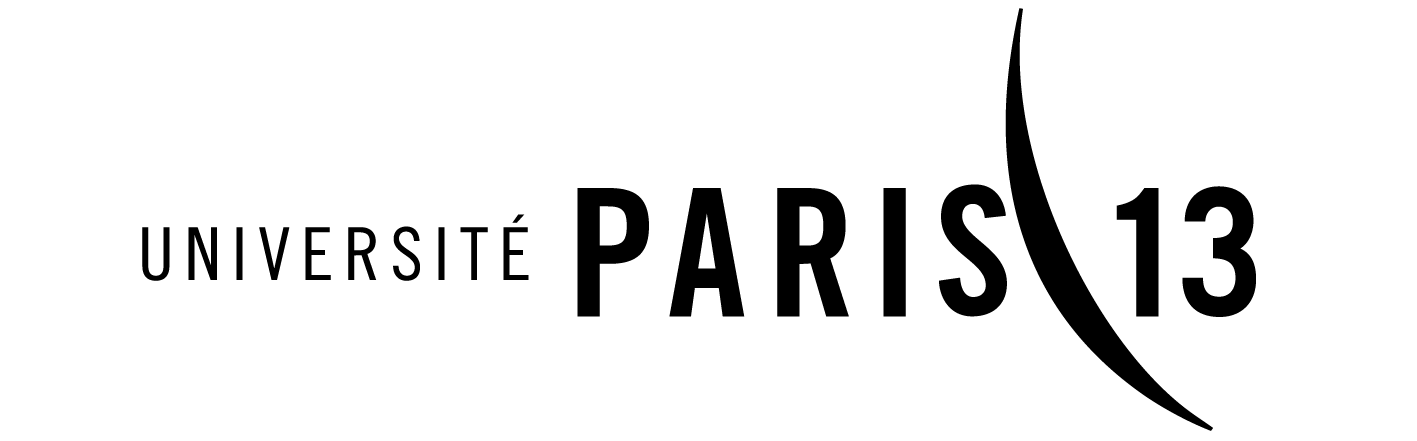
\includegraphics[height = 3cm]{images/logo/P13.png}
  \end{tabularx}
\end{center}
\end{minipage}

\begin{center}
\vspace{\stretch{1}}
% Permet de créer un espace vertical de longueur variable (\stretch) et de "poids" 1
{\Large \textbf{École Doctorale 146 « Sciences, Technologies, Santé – Galilée »}}

\vspace{\stretch{2}}
%Espace vertical variable de poids 2.

{\Huge \textsc{Thèse de doctorat}}

\vspace{\stretch{1}}

{\LARGE Discipline: Mathématiques Appliquées}

\vspace{\stretch{3}}

{\large présentée par}
\vspace{\stretch{1}}

{
    \textbf{{\LARGE Pierre \textsc{Payen}}}\\
}

\vspace{\stretch{2}}
\hrule
\vspace{\stretch{1}}
{\LARGE \textbf{\doctitle}}
\vspace{\stretch{1}}
\hrule
% {\textbf{Version:} \hgid{}}
\vspace{\stretch{1}}

{\Large
dirigée par Olivier \textsc{Lafitte}}

\vspace{\stretch{5}}

{\Large Soutenue le XX/XX/XXXX devant le jury composé de :}

\vspace{\stretch{2}}
{\Large
\begin{tabular}{l@{\hskip 0cm}lll}
M.&Xxxx \textsc{Xxxx} & Xxxx & Rapporteur\\
M\textsuperscript{me}.~&Xxxx \textsc{Xxxx} & Xxxx & Examinateur\\
M.&Olivier \textsc{Lafitte} & LAGA/Paris 13 & Directeur\\
M\textsuperscript{me}.~&Xxxx \textsc{Xxxx} & Xxxx & Président\\
\end{tabular}
}

\end{center}

% \cleardoublepage % pour laisser une page blanche au verso de la page de garde

\newpage

\vspace*{\fill}

%Adresse du labo où la thèse a été faite : demande du ministère !
\noindent
\begin{center}
\begin{minipage}[t]{0.45\textwidth}
LAGA ( UMR 7539 ), Institut Galilée\\
Université Paris 13 \\
99 avenue J.B. Clément \\
93430 Villetaneuse
\end{minipage}%
%
\hfill%
%
\begin{minipage}[t]{0.45\textwidth}
École doctorale 146 « Sciences, Technologies, Santé – Galilée » \\
Université Paris 13 \\
99 avenue J.B. Clément \\
93430 Villetaneuse
\end{minipage}
\end{center}



\end{titlepage}
\hypersetup{pageanchor=true}

\cleardoublepage

\setcounter{secnumdepth}{5} % on numérote tous les niveaux de sections
\setcounter{tocdepth}{1}  % Pas besoin de trop détailler le sommaire ici (chapitres/sections)
\dominitoc
%\tableofcontents
\clearpage
\chapterstar{Acronymes et notations}
%{\color{red}TODO : enlever le \textbackslash{glsaddall}}
%\glsaddall % TODO A retirer
\setlength{\glsdescwidth}{\textwidth}
\printglossaries
~

% %%%%%%%%%%%%%%%%%%%%%%%%%%%%%%%%%%%%%%%%%%%%%%%%%
\mainmatter
\chapter{Introduction et plan de thèse}
\section*{Présentation de la Thèse}\label{pre_th}
\lettrine{C}{ette} thèse de mathématiques appliquées s'intitule ``\doctitle''.
\\

L'objectif de la thèse est d’approfondir la notion de condition d'impédance pour des objets dont la surface est suffisamment régulière constitués d'empilement de matériaux diélectrique de faible indice (au sens de l'optique géométrique).
\\

L’intérêt des conditions d'impédances a été résumé par exemple par \cite{senior_approximate_1995}:
"Prenez par exemple, un objet fini immergé dans un milieu homogène et éclairé par un champ électromagnétique.
Connaissant les propriétés du matériau, il est possible en principe, de trouver les champ rayonnés à l'extérieur de l'objet.
Cependant, ce travail serait grandement facilité si les propriétés pouvait être modélisées par une condition limite ne faisant intervenir que la trace des champs à la surface extérieur de l'objet, de fait, transformant un problème à deux (ou plus) matériaux en un problème à un unique matériau.
"

\subsection*{Introduction}
Nous traitons le problème des équations Maxwell sous forme harmonique, en convention $e^{i\w t}$ pour la dépendance temporelle.


Soit un objet $\O$ de type conducteur parfait de surface $\Gamma$, recouvert d'une couche matériau diélectrique d'épaisseur $d$, caractérisé par sa permittivité diélectrique $\gls{phy-eps}$ et sa perméabilité magnétique $\gls{phy-mu}$ qui peuvent dépendre du point courant et être complexe dans le cas de pertes, l'ensemble se situant dans le vide, telle que la célérité d'une onde électromagnétique soit \gls{phy-c}, et les constantes de permittivité et de perméabilité $\gls{phy-eps}_0$, $\gls{phy-mu}_0$ avec $\eps_0\mu_0 = c^{2}$.


On désigne par \gls{phy-w} la pulsation de l'onde.
En l'absence de charges électriques et magnétiques, les champs éponymes $( \E, \H )$ sont solutions du système d'équations de Maxwell harmonique : 

Le problème de Maxwell dans l'espace s'énonce: \\

Soit $(\E,\H)$ dans $(\Hrot(\O\cup\O^c))^3 \pvect (\Hrot(\O\cup\O^c))^3$
\begin{equation}
\label{eq:pres_th:intro:maxwell}
\left\lbrace \begin{matrix}
\rot \E + i\w\mu' \H &=& 0 \\
\rot \H - i\w\eps' \E &=& 0 \\
\end{matrix} \right.
\quad \text{dans $\O\cup\O^c$}
\end{equation}
A l'extérieur de $\O$, les constantes sont $\eps',\mu'$ sont $\eps_0,\mu_0$ et à l'intérieur elles sont $\eps,\mu$.


Nous complétons ces équations par des conditions aux limites à la surface $S$ de $\O$, supposée régulière et dont on note la normale sortante $\n$:
\begin{itemize}
  \item Les composantes tangentielles des champs sont continues le long d'une surface de discontinuité de $\eps$ et $\mu$ \cite[(2.10) p.~8]{senior_approximate_1995}.

  \begin{align}
  \label{eq:pres_th:intro:transmissions}[\n \pvect \E]_S = 0  \qquad [\n \pvect \H]_S = 0
  \end{align}
\end{itemize}
Dans le cas limite d'un \gls{acr-cep}, les champs $\E$ et $\H$ sont nuls à l'intérieur du conducteur et la composante tangentielle (resp.normale) du champs $\E$ (resp.$\H$) est nulle à l'extérieur.


Enfin comme nous considérons un milieu extérieur non-borné, nous nous dotons de la condition de radiation à l'infini de Silver-Müller afin de définir des solutions en ondes sortantes.


\begin{equation}
\label{eq:pres_th:intro:silver-muller}
\lim_{r\rightarrow\infty}r\left|\left|\sqrt{\eps'}\E - \sqrt{\mu'}\H\pvect\frac{\v r}{r}\right|\right| = 0
\end{equation} 

\subsection*{Les conditions d'impédance comme approximation d'un opérateur de Calderón}

Tel que l'a démontré \cite[Theorem 1., p.~1042]{lafitte_diffraction_1998}, le problème \eqref{eq:pres_th:intro:maxwell}  posé à l'intérieur et à l'extérieur de l'objet, doté de la condition de rayonnement \eqref{eq:pres_th:intro:silver-muller} est équivalent au problème \eqref{eq:pres_th:intro:maxwell} à l'extérieur de l'objet doté de de la condition de rayonnement \eqref{eq:pres_th:intro:silver-muller} et de la \gls{acr-ci} \eqref{eq:pres_th:ci:ci-calderon} sur la surface extérieur de l'objet : 
\begin{equation}
\label{eq:pres_th:ci:ci-calderon}
\n \pvect \E = \mathcal{C}\left(\n \pvect \n \pvect \H\right)
\end{equation}
où $ \mathcal{C}$ est l'opérateur de Calderón.
L'opérateur d'impédance est alors une approximation de cet opérateur de Calderón.

% \subsection*{Plan de la thèse}
% D'abord nous résoudrons le problème de Maxwell dans le cas d'un plan infini recouvert d'une couche mince de matériau diélectrique.
Ce cas permet d'introduire et d'expliciter toutes les notions récurrentes de ce document.


% Puis nous résoudrons le problème de Maxwell avec un objet sphérique.
Pour cela, nous étudierons le problème de Helmholtz (section \ref{sec:helmholtz_scal}) avec un objet sphérique afin d'exhiber des solutions particulière de Maxwell (section \ref{sec:sol_maxwell}), dont nous détaillerons les champs sous la forme d'une série de Mie (section \ref{sec:serie_mie}).
Plusieurs calculs des termes principaux de cette série seront exhibés : solution exacte et injection des \glspl{acr-cioe}.
Ces dernières seront introduites en section  \ref{sec:coeffs_cioe}.


% Nous montrerons alors que l'on peut résoudre les équations de Maxwell grâce à la résolution d'équations intégrales, qui permettent de ne résoudre le problème qu'à la surface du domaine.



\setcounter{mtc}{2} % "Corrige" les minitocs décallés à cause des chapter* (ex : Intro)

\chapter{Impédance d'un empilement multi-couche infiniment plan}
\minitoc
\section{Opérateur d'impédance dans le cas du plan infini}\label{sec:coeffs_ref}

\TODO{Simplifier l'analyse spectrale. Ex: se baser sur \cite[p.~28]{hoppe_impedance_1995}, mais reformuler avec les espaces $L^2$,etc}


Soit un système de coordonnées $(\x,\y,\z)$ tel que le demi-espace des $\z>0$ soit le vide, où une onde est de célérité \gls{phy-c}, de fréquence $\gls{phy-f}$ et de nombre d'onde $\kO=\frac{2\pi f}{c}$  et d'impédance scalaire $\etaO = \sqrt{\frac{\muO}{\epsO}}$ ( de plus $\kO=2\pi f\sqrt{\muO\epsO}$ ).

On définit en tous point la permittivité diélectrique relative $\gls{phy-eps}_p$ et la perméabilité magnétique relative $\gls{phy-mu}_p$, qui sont invariantes par translation dans le matériau.
 Ces constantes adimensionnées peuvent être complexes\footnote{Dans le vide $\eps_0=\mu_0=1.$}.

Le demi-espace $\z<-d$ restant est assimilé à un \gls{acr-cp}.

On utilisera les notations  suivantes dans la suite de cette partie: le vide sera indiqué comme milieu d'indice $0$ , le matériau comme milieu d'indice $1$.

\begin{figure}[h!]
\centering
\begin{tikzpicture}
\coordinate (l) at (-2,0);
\coordinate (r) at (2,0);
\coordinate (m) at ($(r)!0.5!(l)$);

\fill [lightgray] (l) rectangle (2,1) ;
\foreach \t in {-2.2,-2.1,...,2} {
\draw plot[domain=0:0.3] (\t + \x, -\x, 0);
}
\coordinate (ll) at (-2.2,-0.3);
\fill [white] (ll) rectangle (l) ;
\coordinate (rr) at (2,-0.31);
\fill [white] (rr) rectangle (2.3,0) ;


\coordinate (n) at (-4,0);

\coordinate (lt) at (-2,1);
\coordinate (rt) at (2,1);
\coordinate (mt) at ($(rt)!0.5!(lt)$);

\draw (l) -- (r) node [at end,right] {$z = -d$};
\draw (lt)  -- (rt) node [at end,right] {$z = 0$};

\draw (lt) node [above right] {$\eps_0,\mu_0$};
\draw ($(l)!0.5!(lt)$) node [right] {$\eps_1,\mu_1$};

\draw [->] (n) -- ++(0,1) node [at end, right] {$z$};
\draw [->] (n) -- ++(1,0) node [at end, right] {$x$};

\draw (n) circle(0.1cm) node [below=0.1cm] {$y$};
\draw (n) +(135:0.1cm) -- +(315:0.1cm);
\draw (n) +(45:0.1cm) -- +(225:0.1cm);

%\draw [->>,thick] (lt) ++ (1,1) -- (mt) ;


\end{tikzpicture}
\caption{schéma du plan infini}
\end{figure}\label{fig:tikz:plan}

\subsection{Objectif}
On cherche à obtenir l'opérateur différentiel \gls{ope-imp}, tel que l'on ait la relation,

\begin{equation}
\label{eq:coeff_ref:intro:ci}
-\n \pvect \n \pvect \E(\x,\y,0) = \mathcal{Z}( \n \pvect H)(\x,\y,0)
\end{equation}

%Le premier cas d'étude est celui du plan infini. Il permet de résoudre facilement le problème de Maxwell \eqref{eq:maxwell} et de déterminer l'expression de la la condition d'impédance (\gls{acr-ci}).
%%%% SECTION HYPOTHESES
\begin{hyp}[Hypothèses simplificatrices]{}~\\
\begin{enumerate}
    \item On suppose que les solutions s'écriront comme $Ce^{i(k_\x\x +k_\y\y+k_\z\z)}, C\in\C$.
    \item Comme le plan est infini et quitte à redéfinir les axes cartésiens, on peut supposer que l'onde se propage suivant le vecteur $\v k_p = (k_{\x,p},0,k_{\z,p})$ : pas de dépendance en $\y$ et $k_\y$.
\end{enumerate}
\end{hyp}

On note $\eta_p = \sqrt{\frac{\mu_p}{\eps_p}}$ et $\nu_p = \sqrt{\mu_p \eps_p}$.
On a donc $k_p = \kO\nu_p$\footnote{Évidemment $k_0 = \kO$} et $k_{z,p} = \sqrt{k_p^2 - k_{x,p}^2}$.

\begin{hyp}[Principe de superposition]{}~\\
La solution générale est une combinaison linéaire de deux problèmes: 
\begin{enumerate}
    \item \gls{acr-te} : $\E = (0,E_y,0)$.
    \item \gls{acr-tm} : $\H = (0,H_y,0)$. 
\end{enumerate}
\end{hyp}

\subsection{Solutions}

\begin{tcolorbox}
\centering
La dépendance temporelle est en $e^{i \omega t}$, et l'on identifie $\H \equiv \etaO \H$.
\end{tcolorbox}


Soit $(\E,\H)$ dans $(\Hrot(\O))^3 \times (\Hrot(\O))^3$. 

Alors $(\E,\H)$ sont solutions de Maxwell si 
\begin{align}
\label{eq:coeffs_ref:maxwell-E}
\trot \E + i k_p \eta_p \H &= 0 && \text{dans $\O$}\\
\label{eq:coeffs_ref:maxwell-H}
\trot \H - i \frac{k_p}{\eta_p} \E &= 0 && \text{dans $\O$}
\end{align}

Les équations de Maxwell donnent dans chacun des domaines (indicé par le $p = \lbrace0,1\rbrace$) et pour chacune des polarisations:

\Gls{acr-te}: $ \E(\x,\z) = (0,E_y,0), \H(\x,\y) = (H_x,0,H_z)$. 
\[
\left\lbrace 
\begin{matrix}
-\d_{\z} E_\y + i k_p \eta_p H_\x & = & 0 \\
\d_{\x} E_\y + i k_p \eta_p H_\z &= & 0 \\
\d_{\z} H_\x- \d_{\x} H_\z - i\frac{k_p}{\eta_p} E_\y & = & 0\\
\end{matrix}
\right.
\Rightarrow
\left\lbrace
\begin{matrix}
\d_{\z\z}^2 E_\y + \d_{\x\x}^2 E_\y + k_p^2 E_\y = 0\\
H_\x = \frac{\d_{\z} E_\y}{i k_p \eta_p }\\
H_\y =  -\frac{\d_{\x} E_\z}{i k_p \eta_p }
\end{matrix}
\right.
\]

\Gls{acr-tm} : $ \E(\x,\z) = (E_\x,0,E_\z), \H(\x,\z) = (0,H_\y,0)$. 
\[
\left\lbrace 
\begin{matrix}
\d_{\z} E_\x - \d_{\x} E_\z + i k_p \eta_p  H_\y &= & 0 \\
- \d_{\z} H_\y - i\frac{k_p}{\eta_p} E_\x & = & 0\\
\d_{\x} H_\y -i\frac{k_p}{\eta_p} E_\z &=&0\\
\end{matrix}
\right.
\Rightarrow
\left\lbrace
\begin{matrix}
\d_{\z\z}^2 H_\y + \d_{\x\x}^2 H_\y + k_p^2 H_\y = 0\\
E_\x = -\eta_p\frac{\d_{\z} H_\y}{i k_p}\\
E_\y = \eta_p\frac{\d_{\x} H_\y}{i k_p}
\end{matrix}
\right.
\]

On obtient alors une équation de Helmholtz à résoudre respectivement pour $E_\y$ et $H_\y$.

Dans la suite, nous allons donc considérer comme inconnu $U$, solution du problème suivant : 

\begin{equation}
\d_{\z\z}^2 U + \d_{\x\x}^2 U + k_p^2 U = 0 \quad \text { dans $\O\cup\O^c$}
\end{equation}

% \begin{hyp}[Hypothèses simplificatrices 2]{Passage dans le domaine de Fourier}\\
%   Par définition d'une onde plane $U(x_1,x_2,\z)$, on a la propriété suivante sur sa transformée de Fourier $ U(k_{1,i},k_{2,i},k_{3,i})$:
% \[
%  \d_j { U}(\v \kO) = ik_{j,i}  U(\v \kO)
% \]
% \end{hyp}

% 
% \iffalse
% \subsection{Onde plane et transformée de Fourier}
% Une onde plane harmonique (dépendance $e^{i\wt}$) est de type $U(x_1,x_2,\z) = U_0e^{i(k_1x_1+k_2x_2+k_3\z)}$, dont on remarque que . 
% 
% Or une propriété de la transformée de Fourier $ U$ de $U$ est ${ \d_j U}(\xi) = i\xi_j  U$. 
% Donc on peut faire l'analogie entre l'hypothèse d'une onde plane et la transformée de Fourier de $U$,
%  avec l'analogie $\xi_j \leftrightarrow  k_j$.
% \fi
% %%%% SECTION Z
% \subsection{Impédance de surface pour une couche de matériau}
% Comme le plan est infini, on peut prendre les transformées de Fourier des 2 équations trouvées précédemment afin que les opérateur différentiels issus des équations de Maxwell deviennent des coefficients multiplicatifs. On peut alors rechercher une CI tel que $\mathcal{Z} = Z\operatorname{Id}$ et on note $ \kO = \w^2 \eps_p \mu_p$.
% 
% Rappellons que dans le domaine de Fourier, ${ \d_j U}(\xi) = i\xi_j  U$ %(on rappelle que $k_{\z,1} \leftrightarrow k_1$)

%%% OLD FOURIER

% Comme $(\E,\H)$ sont dans $L_2(\O)$, ils admettent une transformée de Fourier $( \E,  \H)$ dans $L^2$ et l'on a

% \[
%   U(\x,\y,\z) = \frac{1}{2\pi} \int_{\R^3}  U (k_\x,k_\y,k_\z) e^{i(k_\x\x +k_\y\y+k_\z\z)} dk_\x dk_\y dk_\z
% \]

% Le problème que l'on veut résoudre est maintenant le suivant:
% \begin{equation}
%   \d_{\z\z}^2  U + k_{\z,p}^2  U = 0 \quad \text { dans $\O\cup\O^c$}
% \end{equation}

% Et dont les solutions de l'équation ci-dessus sont

% \[
% \hfill U_p(k_z\z) = A_p e^{-ik_{\z,p} \z}  + B_p e^{ik_{\z,p} \z}
% \]

% On suivra comme convention qu'en polarisation TE, $ U =  E_\y$ et en polarisation TM, $ U =  H_\y$, l'autre champ découlant des équations de Maxwell.

Grâce à l'hypothèse sur la forme des solutions

\[
\d_{\x} U(\x,\z) = ik_\x U(\x,\z)
\]

Le problème que l'on veut résoudre est maintenant le suivant:
\begin{equation}
\d_{\z\z}^2 U + k_{\z,p}^2 U = 0 \quad \text { dans $\O\cup\O^c$}
\end{equation}

Et dont les solutions de l'équation ci-dessus sont

\[
\hfill U(\z) = A_p e^{-ik_{\z,p} \z}  + B_p e^{ik_{\z,p} \z}
\]

On suivra comme convention qu'en polarisation TE, $ U = E_\y$ et en polarisation TM, $ U = H_\y$, l'autre champ découlant des équations de Maxwell.


Les conditions limites sur le matériau vont permettre de déterminer les valeurs des constantes $A_p, B_p$.
\begin{itemize}
    \item 
    Conducteur parfait (\gls{acr-cp})\footcite[p.~217]{morse_methods_1953} : $\v{E_t}(-d) = 0  $
    \item 
    Continuité des champs tangents: $
    \left\lbrace 
    \begin{matrix}
    [ E_t]_{\z=0} &=& 0 \\
    [ H_t]_{\z=0} &=& 0 
    \end{matrix}
    \right.$
\end{itemize}

%%%  TE
Nous allons alors calculer les champs tangents, utiliser les conditions limites puis la condition d'impédance pour obtenir le multiplicateur de Fourier associé à l'opérateur d'impédance.

\TODO{Trouver quelque chose de mieux que le tableau. Arrêter TE, TM => cas général 3D ?}

\begin{center}
\begin{tabular}{| C | C | C |}
\hline
& \text{\textbf{TE}} & \text{\textbf{TM}} \\
\hline\hline

\v { E_t} & \left(A_p e^{-ik_{\z,p} \z}  + B_p e^{ik_{\z,p} \z}\right) \v e_2 &  \frac{k_{\z,p}\eta_p}{k_p}\left( A_p e^{-ik_{\z,p} \z} - B_p e^{ik_{\z,p}z}\right) \v e_1\\
\hline

\v { H_t} &\frac{k_{\z,p}}{k_p\eta_p} \left(-A_p e^{-ik_{\z,p} \z}  + B_p e^{ik_{\z,p} \z}\right) \v e_1 & \left(A_p e^{-ik_{\z,p} \z} + B_p e^{ik_{\z,p} \z}\right) \v e_2\\
\hline

\E_t(-d) = 0 & A_1 = -B_1e^{-ik_{\z,1}2d} &  A_1 = B_1e^{-ik_{\z,1}2d}\\
\hline

\multirow{2}{*}{$\E_t(0)=Z\n\times \H(0)$} & B_1\left(1-e^{-ik_{\z,1}2d}\right) & B_1\left( 1 - e^{-ik_{\z,1}2d} \right)\frac{k_{\z,1}\eta_1}{k_1}  \\
& =  Z\frac{k_{\z,1}}{k_1\eta_1}B_1\left(1+e^{-ik_{\z,1}2d}\right) & = Z\left(e^{-ik_{\z,1}2d} + 1\right)B_1\\
\hline
\hline
Z & \dfrac{k_1\eta_1}{k_{\z,1}}i\tan(k_{\z,1}d) & \dfrac{k_{\z,1}\eta_1}{k_1}i\tan(k_{\z,1}d) \\
\hline
\end{tabular}
\end{center}

\subsection{Matrice diagonale d'impédance dans le domaine de Fourier}

L'opérateur $Z$ est la matrice $diag(Z_{TE},Z_{TM})$:
\begin{align}
\notag Z&=\dfrac{i\eta_1}{k_1^2}\frac{k_1\tan(k_{\z,1}d)}{k_{\z,1}}(k_1^2 I - L_R ) \\
&=\dfrac{i\eta_1}{k_1^2}P(k_1^2 I - L_R )\label{eq:coeff_ref:mat_z:imped}
\end{align}

où $L_R = diag(0,k_{\x,1}^2)$. C'est la forme que l'on retrouve dans \cite{marceaux_high-order_2000}.

%%%% SECTION REFLEXION
\subsection{Coefficients de réflexions}
Le rapport $R=B_0/A_0$ est appelé coefficient de réflexion. On cherche à l'exprimer en fonction de l'impédance de surface $Z$. On réutilise les équations de continuités: 

\begin{center}
\begin{tabular}{| C | C | C |}
\hline
& \text{\textbf{TE}} & \text{\textbf{TM}} \\
\hline\hline

1+R & \dfrac{B_1(1-e^{-ik_{\z,1}2d})}{A_0}& \dfrac{B_1(1+e^{-ik_{\z,1}2d})}{A_0} \\ 
\hline

-1+R & \dfrac{k_{\z,1}\mu_0 B_1(1+e^{-ik_{\z,1}2d})}{k_{\z,0} \mu_1 A_0} & \dfrac{k_{\z,1}\eps_0 B_1(1-e^{-ik_{\z,1}2d})}{k_{\z,0} \eps_1A_0}\\
\hline
\multirow{2}{*}{$\frac{1+R}{-1+R}$}  & -\frac{k_{\z,0} \mu_1}{k_{\z,1} \mu_0}i\tan(k_{\z,1} d) & -\frac{k_{\z,0} \eps_1}{k_{\z,1}\eps_0}\dfrac{1}{i\tan(k_{\z,1}d)}\\
& =\frac{k_{\z,0}Z_{TE}}{k_0\eta_0} & =\frac{k_{\z,0}\eta_0}{k_0Z_{TM}}\\
\hline
\hline
R & \frac{k_{z,0}Z_{TE}-1}{k_{z,0}Z_{TE}+1} & \frac{k_{z,0}-Z_{TM}}{k_{z,0}+Z_{TM}} \\
\hline
\end{tabular}
\end{center}

\subsection{Ondes évanescentes}

On note $s=\frac{k_{x,p}}{k_p}$. Si $s>1$ alors $k_{z,p} = k_p\sqrt{\nu_p^2-s^2}$ devient complexe\footnote{Sinon on peut noter $s=\sin(\theta_{inc})$}.
La partie imaginaire de ce complexe crée une exponentielle réelle dans la solution générale. On obtient donc des ondes exponentiellement décroissante dans la direction des $\z$ croissant. Ces ondes sont appelées évanescentes.

%%% SECTION MULTICOUCHE
\subsection{Cas d'un empilement de matériau}

Un empilement peut-être résolue itérativement: étant donnée une condition d'impédance en $\z$, on va déduire la condition d'impédance en $\z+d$.

En effet, on peut toujours se ramener dans le cas du plan infini avec une couche, c'est à dire avec la condition d'impédance connue en $\z=-d$ et celle que l'on cherche en $\z=0$

On suppose que l'on ait une condition d'impédance en $\z=-d$\[
\v { E_{tan}}=Z_d \, \n \pvect  \H
\]


\begin{align*}
\gamma_{TE} := \dfrac{k_{\z,1}}{k_1} \dfrac{Z_d}{\eta_1} \qquad
\gamma_{TM} := \dfrac{k_{\z,1}}{k_1}  \frac{\eta_1}{Z_d}  \qquad
\alpha(\gamma) = \frac{1-\gamma}{1+\gamma}
\end{align*}

\begin{center}
\begin{tabular}{| C | C | C |}
\hline
& \text{\textbf{TE}} & \text{\textbf{TM}} \\
\hline\hline

\v { E_t} & \left(A_p e^{-ik_{\z,p} \z}  + B_p e^{ik_{\z,p} \z}\right) \v e_2 &  \frac{k_{\z,p}\eta_p}{k_p}\left( A_p e^{-ik_{\z,p} \z} - B_p e^{ik_{\z,p}z}\right) \v e_1\\
\hline

\v { H_t} &\frac{k_{\z,p}}{k_p\eta_p} \left(-A_p e^{-ik_{\z,p} \z}  + B_p e^{ik_{\z,p} \z}\right) \v e_1 & \left(A_p e^{-ik_{\z,p} \z} + B_p e^{ik_{\z,p} \z}\right) \v e_2\\
\hline

{\E_t}(-d) = Z_d \n\times\H(-d) & A_1 = -\alpha(\gamma_{TE}) B_1e^{-ik_{\z,1}2d} &  \\
\hline

\multirow{2}{*}{$\E_t(0)=Z\n\times \H(0)$} & B_1\left(1-\alpha(\gamma_{TE})e^{-ik_{\z,1}2d}\right) &   \\
& =  Z\frac{k_{\z,1}}{k_1\eta_1}B_1\left(1+\alpha(\gamma_{TE})e^{-ik_{\z,1}2d}\right) & \\
\hline
\hline
Z & \dfrac{k_1\eta_1}{k_{\z,1}}\tanh\left(ik_{\z,1}d-\frac{\log(\alpha(\gamma_{TE}))}{2}\right) &  \\
\hline
\end{tabular}
\end{center}
\[
\\
P = \dfrac{ik_1}{k_{\z,1}}diag\left(\dfrac{1-\alpha(\gamma_{TE}) e^{ik_{\z,1}2d}}{1+\alpha(\gamma_{TE}) e^{ik_{\z,1}2d}},\dfrac{1-\alpha(\gamma_{TM}) e^{ik_{\z,1}2d}}{1+\alpha(\gamma_{TM}) e^{ik_{\z,1}2d}}\right)
\]
% {
%   \color{blue}Valeur particulière en $Z_d = -\gamma$. À étudier si l'occasion se présente. 
% }
Alors, la condition d'impédance en $\z=0$ est
\begin{align}
\label{eq:coeff_ref:mult_couch:imped}
Z = i \dfrac{\eta_1}{k_1^2}P\left(k_1^2 I-\LR\right)
\end{align}
où $\LR$ est défini de la même façon qu'en \eqref{eq:coeff_ref:mat_z:imped}

\section{Calcul des coefficients des CIOEs}\label{sec:coeffs_cioe}
%{
%\color{red} Terminer cette partie : noyau de Q pour dire si sdp.
%}

Nous allons maintenant étudier comment approcher l'opérateur d'impédance. Ce travail complète les résultats de \cite[Annexe~A]{stupfel_implementation_2015} car nous caractérisons l'image et le noyau de la fonctionnelle.

On cherche à déterminer les coefficients des CIOE \((a_0,a_1,b) \in \CC^3\) qui permettent d'approcher la condition d'impédance \eqref{eq:coeff_ref:mat_z:imped}.

% \begin{equation}
% \label{eq:cioe}
% %-\n \pvect \n \pvect \E = \gls{ope-imp} \left( \n \pvect \H \right)
% %\approx
% -\left(1 + b t \right)\n \pvect \n \pvect \E = \left(a_0 + a_1 t \right)\n \pvect \H
% \end{equation}

On se place en un point de la surface.
Si la surface y est suffisamment régulière, on peut trouver un voisinage de ce point tel que le problème à résoudre soit celui étudié en section \ref{sec:coeffs_ref}.

\subsection{Formulation exacte dans le cadre de l'approximation plan tangent}

Soit \(s\) tel que \(k_{x,0} = k_0s\)\footnote{Si  \(s \le 1, s=\sin(\theta)\), angle d'incidence par rapport à la normale au plan tangent.}. Soit \(t := \frac{s^2}{\nu^2}\). Alors
\begin{align*}
  \text{TE: } \mathcal Z_{th}(t) &= i\eta \frac{\tan\left(kd\sqrt{1+\frac{t}{\nu^2}}\right)}{\sqrt{1+\frac{t}{\nu^2}}}\\
  \text{TM: } \mathcal Z_{th}(t) &= i\eta \frac{\tan\left(kd\sqrt{1+\frac{t}{\nu^2}}\right)}{\sqrt{1+\frac{t}{\nu^2}}}(1+\frac{t}{\nu^2})
\end{align*}
%%%%%% SECTION MOINDRE CARRE

La méthodologie est la suivante : étant donné plusieurs \(s_j\) entre \(0\) et \(s_{\max}\)\footnote{Le choix du \(s_{\max}\) est réalisé en calculant l'erreur L2 relative entre les coefficients de réflexions exactes et ceux des CIOEs}, on va minimiser la distance entre le \(Z\) et le \(\mathcal{Z}_{th}\).

On dispose de \(N\) observations de \(\mathcal Z_{th} : Z_j = \mathcal Z_{th}(t_j)\), on note \(X = (a_0,a_1,b) \in \CC^3\).
\subsection{Calcul des coefficients par résolution d'un problème d'optimisation}
\subsubsection{Fonctionnelle à minimiser}
Soit \(f:\CC^3 \rightarrow \CC\)
\[
f_t(X) = a_0 + a_1 t - b t \mathcal Z_{th}(t)
\]
On cherche alors à minimiser la distance de \(f\) à \(\mathcal Z_{th}\)  : on cherche \(X_{opt}\in \CC^3\) tel que
\[
X_{opt} = \text{argmin}_X \left( \frac{1}{2}\sum_{j=1}^{N} | f_{t_j}(X) - Z_j|^2 \right)
\]

\subsection{Calcul des coefficients par résolution d'un système linéaire}
On peut écrire le problème à résoudre comme
\begin{align*}
	MX &= Z\\
	M &=
	\begin{bmatrix}
		1 & t_1 & -t_1Z_1 \\
		\vdots & \vdots & \vdots \\
		1 & t_N & -t_NZ_N
	\end{bmatrix}
\end{align*}

On résout ce genre de système non inversible en utilisant la transposée conjuguée.
\begin{equation}
   \conj{M^t}MX = \conj{M^t} Z
\end{equation}
Ce genre de solution est équivalent à la résolution d'un système par moindre carré \cite{penrose_best_1956} :
\begin{equation}
  X_{opt} = \left(\conj{M^t}M\right)^{-1}\conj{M^t} Z = M^+ Z
\end{equation}

\subsubsection{Formulation sous forme quadratique}\label{sec:formQ}

Soit \(\left<.,.\right>\) le produit scalaire associée à la norme \(||.||_2\) (\(\left<a,a\right> = ||a||_2^2 = \sum_{j=1}^N|a_j|^2\)).

\begin{prop}
Il existe une matrice \(Q\), un vecteur \(P\) et un scalaire \(D\) tel que:

\[
\frac{1}{2}\sum_{j=1}^N |f_{\xi_j}(X) -Z_j|^2 = \left<Q X,X\right> -2\left<P,X\right> +D
\]
\end{prop}
\begin{proof}
\begin{align*}
\sum_{j=1}^N |f_{t_j}(X) -Z_j|^2&= ||MX-Z||^2\\
&= \left<MX-Z,MX-Z\right>\\
&=\left<\conj{M^t}MX,X\right> - 2\left<\conj{M^t}Z,X\right> + \left<Z,Z\right>\\
&= 2\left<Q X,X\right> -\left<P,X\right> +2D
\end{align*}

Si Q est inversible alors le minimum de cette fonctionnelle est atteint en \(X_{opt} = Q^{-1}P\)

\end{proof}

Si l'on cherche des inconnus réelles, on a :

Soit \((x_i)_{i=1..6} \in \RR^6\),
\begin{align*}
g_t(x) &=
\x_1 + \x_3 t - \left(x_5 Z_{th}(t)' - x_6 Z_{th}(t)''\right)t  \\
&+ i\left(
\x_2 + \x_4 t - \left(x_5 Z_{th}(t)'' + x_6 Z_{th}(t)'\right)t
\right)
\end{align*}
où \(z'= \Re{z}, z''=\Im{z}\).

alors de la même manière, il existe une matrice \(Q\), un vecteur \(P\) et un scalaire \(D\) tel que
\[
\sum_{j=1}^N|f_{t_j}(X) -Z_j|^2  = \sum_{j=1}^N|g_{t_j}(x) -Z_j|^2 = \left<Q x,x\right> -2\left<P,x\right> + D
\]

De plus, on a \(Q = \sum_{j=1}^N Q_j, P = \sum_{j=1}^N P_j ,D=\sum_{j=1}^N D_j\) où
\[
Q_j =
\begin{bmatrix}
1 & 0 & t_j & 0 & -t_jZ_j' & t_jZ_j'' \\
& 1 & 0 & t_j & -t_jZ_j'' & -t_jZ_j' \\
&   & t_j^2 & 0 & -t_j^2Z_j' & t_j^2Z_j'' \\
&   &  & t_j^2 & -t_j^2Z_j'' & -t_j^2Z_j' \\
&   &  &  & t_j^2|Z_j|^2 & 0 \\
&   &  &  &  & t_j^2|Z_j|^2 \\
\end{bmatrix}
,\quad
P_j =
\begin{bmatrix}
Z_j' \\ Z_j'' \\ t_j Z_j' \\ t_j Z_j''  \\ -t_j |Z_j|^2  \\ 0
\end{bmatrix}
,\quad
D_j = |Z_j|^2
\]

Et \(Q_j\) est une matrice symétrique par définition du produit scalaire, positive par définition du module:
\[
\forall x \in \RR^6, q(x) := \left<Q_jx,x\right> = |g_t(x)|^2 \ge 0
\]
Mais elle n'est pas définie : il existe \(x \not = 0\) tel que \(q(x) = 0\) (ex, \(x = (1,0,-1/t_j,0,0,0)\)).

Cependant, la matrice Q semble définie pour \(N \ge 6\) ce qui a été constaté numériquement.

\begin{TODO}
  Faire le ménage dans cette étude, il y a des choses non finis et/ou inutile
\end{TODO}
% \subsection{Etude de la forme quadratique}\label{sec:etud_Q}

% En permutant les composantes du vecteur \(x\), on passe à \(\tilde x = (a_0',a_1',b',a_0'',a_1'',b'')^t\) et pour obtenir \(x^tQ_jx = {\tilde x}^t\tilde{Q_j} \tilde{x}\) avec
% \[
%   \tilde{Q_j} =
%   \begin{bmatrix}
%     1 &  t_j & -{t_j Z'} &0 &0 &{t_j Z''}\\
%       & {t_j^2} & -{t_j^2Z'} & 0 &0 & {t_j^2Z''}\\
%       & & {t_j^2|Z|^2} & -{t_j Z''} & -{t_j^2Z''} & 0\\
%       & & & 1 & t_j & -{t_j Z'} \\
%       & & & & {t_j^2} & -{t_j^2 Z'} \\
%       & & & & & {t_j^2|Z|^2}
%   \end{bmatrix}, \text{ symétrique }
% \]

% On définit les matrices \(A,B\) respectivement symétriques et antisymétriques telles que \(\tilde{Q_j} = \begin{bmatrix} A & B \\ B^t & A\end{bmatrix}\).
% % Cherchons les valeurs propres de \(\tilde{Q_j}\). Par soucis de simplicité, on identifie le scalaire 1 à la matrice identité.

% % \begin{align}
% %   \ddet(\tilde{Q_j} -\lambda) = \ddet(A-\lambda) \ddet(A-\lambda - B(A-\lambda)^{-1}B^t)\label{eq:detQj}
% % \end{align}

% \begin{tcolorbox}
% \centering
% \textbf{On définit et utilise dans ce qui suit}
% \[{x_j} = t_j,\; {y_j} = t_j Z_j',\; {z_j} = t_j Z_j''\]
% \end{tcolorbox}


% \subsubsection{Caractérisation de l'image et du noyau de la sous-matrice A}
% Soit \(\mathcal B = (\v{e_1},\v{e_2},\v{e_3})\) la base canonique\\
% Soit \(A_\mathcal{B} = \begin{bmatrix}
%  1 & {x_j} & -{y_j} \\
%  {x_j} & {x_j}^2 & -{x_jy_j} \\
%  -{y_j} & -{x_jy_j} & {y_j}^2 + {z_j}^2
% \end{bmatrix}\)\\
% Soit \({\v{v_j}} := \frac{1}{\sqrt{1 + {x_j}^2}}\begin{bmatrix} 1&{x_j}&0\end{bmatrix}^t, {\v{u_j}} = \frac{1}{\sqrt{1+{x_j}^2}}\begin{bmatrix} -{x_j} & 1 & 0 \end{bmatrix}^t\).
% \begin{prop}
%   \begin{align*}
%     \Img(A) &= \Vect{{\v{v_j}},\v{e_3}}\\
%     \Ker(A) &= \Vect {\v{u_j}}
%   \end{align*}
% \end{prop}

% \begin{proof}
%   On a : \(A_\mathcal{B} = \begin{bmatrix} 1 & {x_j} & -{y_j} \\ {x_j} & {x_j}^2 & -{x_jy_j} \\ -{y_j} & -{x_jy_j} & {y_j}^2 + {z_j}^2\end{bmatrix}\)

%   On remarque que les 2 premières lignes sont linéairement dépendantes, \((-{x_j}, 1, 0)^t\) appartient au noyau donc \textbf{le rang de \(A\) est alors au plus de 2.}

%   Soit \(e_i\) un vecteur de la base canonique.

%   On remarque que \(A\v{e_1} = ( 1, {x_j} , -{y_j})^t =: \v{\tau}\). Donc \(\v{\tau}\) appartient à l'image de A.

%   De plus, \(A\v{e_2} = {x_j}\v{\tau}\), puis \(A\v{e_3} = -{y_j}\v{\tau}+{z_j}^2\v{e_3}\). On peut en déduire que \(A(\v{e_3} + {y_j} \v{e_1}) = {z_j}^2 \v{e_3}\).

%   Donc \(\v{e_3}\) appartient à l'image de \(A\). La famille \((\v{\tau},\v{e_3})\) est libre et génératrice, l'image est au plus de dimensions 2 donc c'est une base de l'image.

%   On va prendre alors la base orthonormale associée :

%   Soit \[
%   {\v{v_j}} := \frac{\v{\tau}}{||\v{\tau}||} = \frac{1}{\sqrt{1 + {x_j}^2 +{y_j}^2}}\begin{bmatrix} 1\\{x_j}\\-{y_j}\end{bmatrix}\]
%   \[{\v{v_j}}^t := \v{e_3} - (\v{e_3}\cdot {\v{v_j}}){\v{v_j}} = \frac{1}{1+{x_j}^2+{y_j}^2}\begin{bmatrix} {y_j} \\ {x_jy_j} \\ 1 + {x_j}^2\end{bmatrix}\]

%   Mais cette base n'est pas pratique : en effet \(A\v{v_j} = \sqrt{1+{x_j}^2+{y_j}^2} {\v{v_j}} - {y_j} {z_j}^2 \v{e_3}\). \textbf{On ne voit pas \({\v{v_j}}^t\) apparaître.}. Mais puisque que \(\v{e_3}\) apparaît dans l'image, on va supprimer sa composante de \({\v{v_j}}\):

%   Soit \({\v{v_j}} := \frac{1}{\sqrt{1 + {x_j}^2}}\begin{bmatrix} 1\\{x_j}\\0\end{bmatrix}\).
%   Alors
%     \begin{align*}
%     A \v{e_1} &= \sqrt{1+{x_j}^2}{\v{v_j}} - {y_j} \v{e_3}\\
%     A \v{e_2} &= {x_j}\sqrt{1+{x_j}^2}{\v{v_j}} -{x_jy_j} \v{e_3}\\
%     & \Rightarrow A {\v{v_j}} = (1+{x_j}^2) {\v{v_j}} - {y_j}\sqrt{1+{x_j}^2} \v{e_3}\\
%     A \v{e_3} &= -{y_j}\sqrt{1+{x_j}^2}{\v{v_j}} +({y_j}^2+{z_j}^2) \v{e_3}\\
%     \intertext{La famille \(({\v{v_j}},\v{e_3})\) est libre et génératrice, l'image est au plus de dimensions 2 donc c'est une base de l'image. On a en définitive }
%     \Img(A) &= \Vect{{\v{v_j}},\v{e_3}}\\
%     \Ker(A) &= \Vect {\v{u_j}}
%   \end{align*}
% \end{proof}

% \begin{prop}
%   Soit R la forme réduite de A dans \(\mathcal{B'}= (\v{e_3},{\v{v_j}},{\v{u_j}})\)

%   \[
%     R =
%     \begin{bmatrix}
%       {y_j}^2+{z_j}^2 & -{y_j}\sqrt{1+{x_j}^2} & 0   \\
%       -{y_j}\sqrt{1+{x_j}^2} &1+ {x_j}^2 &0 \\
%       0 & 0 & 0
%     \end{bmatrix}
%   \]
%   Avec la matrice de passage entre les bases \(\mathcal B\) et \(\mathcal B'\):

%   \[
%     P_{\mathcal B' \rightarrow \mathcal B} = \frac{1}{\sqrt{1+{x_j}^2}}
%     \begin{bmatrix}
%       0 & 1 & -{x_j} \\
%       0 & {x_j} & 1 \\
%       \sqrt{1+{x_j}^2} & 0 &0
%     \end{bmatrix}
%   \]
% \end{prop}

% \subsubsection{Caractérisation de l'image et du noyau de la sous-matrice B}
% Soit \(B = \begin{bmatrix} 0 & 0 & {z_j} \\ 0 & 0 & {x_jz_j} \\ -{z_j} & -{x_jz_j} & 0\end{bmatrix}\)
% \begin{prop}
%   \begin{align*}
%     \Img(B) &= \Img(A) \\
%     \Ker(B) &= \Ker(A)
%   \end{align*}
% \end{prop}

% \begin{proof}
%   On remarque que de nouveau \({\v{u_j}} \in \Ker(B)\).

%   En appliquant le même raisonnement
% \begin{align*}
%  B \v{e_1} &= -{z_j} \v{e_3}\\
%  B \v{e_2} &= -{x_jz_j} \v{e_3}\\
%  B {\v{v_j}} &= -{z_j}\sqrt{1+{x_j}^2}\v{e_3}\\
%  B \v{e_3} &= {z_j}\sqrt{1+{x_j}^2}{\v{v_j}}
% \end{align*}
%  donc par les mêmes arguments que précédemment, \(({\v{v_j}},\v{e_3})\) appartiennent à l'image et alors B est totalement déterminée..
% \end{proof}

% \begin{defn}
%   B s'exprime dans la base \(\mathcal{B'}= (\v{e_3},{\v{v_j}},{\v{u_j}})\) comme
%   \[
%     B_\mathcal{B'} = {z_j}\sqrt{1+{x_j}^2}
%     \begin{bmatrix}
%       0 & -1 & 0 \\
%       1 & 0 & 0\\
%       0 & 0 & 0
%     \end{bmatrix}
%   \]
% \end{defn}

% \subsubsection{Caractérisation du noyau et de l'image de \(Q_j\)}

% \newcommand{\sqx}{\sqrt{1+{x_j}^2}}

% Soient
% \begin{align*}
% V_{j,1} &= \begin{bmatrix}  \sqx {\v{v_j}} - {y_j} \v{e_3} \\ -{z_j} \v{e_3} \end{bmatrix}\\
% V_{j,2} &= \begin{bmatrix} {z_j} \v{e_3} \\  \sqx {\v{v_j}} - {y_j} \v{e_3}\end{bmatrix}\\
% U_{j,1} &= \begin{bmatrix} 0_{\RR^3} \\ {\v{u_j}} \end{bmatrix}\\
% U_{j,2} &= \begin{bmatrix} {\v{u_j}} \\0_{\RR^3} \end{bmatrix}\\
% U_{j,3} &= \sqrt{\frac{z_j^2}{1+x_j^2 +y_j^2+z_j^2}}\begin{bmatrix} \frac{y_j}{z_j}{\v{v_j}} + \frac{\sqx}{z_j}\v{e_3}{\v{v_j}}\end{bmatrix}\\
% U_{j,4} &= \sqrt{\frac{1}{1+x_j^2 +y_j^2+z_j^2}}\begin{bmatrix} -z_j\v{v_j} \\ y_j\v{v_j} + \sqx \v{e_3}\end{bmatrix}
% \end{align*}
% %TODO ORTHONORMALISER POUR AVOIR UNE BASE DE R6. V1.U4 != 0 V2.U3 !=0

% {
% \color{red}
% Ces six vecteurs ne forment pas une base de R6 car V1.U4 != 0 V2.U3 != 0. A revoir !
% }

% \begin{prop}
%   \begin{align*}
%     \Img(Q_j) &= \Vect{V_{j,1},V_{j,2}} \\
%     \Ker(Q_j) &= \Vect{U_{j,1},U_{j,2},U_{j,3},U_{j,4}}
%   \end{align*}
% \end{prop}

% \begin{proof}


% On vérifie facilement que \(U_{j,1}\) et \(U_{j,2}\) appartiennent au noyau puisque \(\v{u_j}\) appartient au noyau de \(A\) et de \(B\).

% De même \(V_{j,1} = Q_j\begin{bmatrix}\v{e_1}\\0_{\RR^3}\end{bmatrix}\not =0\) et \(V_{j,2} = Q_j\begin{bmatrix}0_{\RR^3}\\\v{e_1}\end{bmatrix} \not= 0\) et \(V_{j,1}\cdot V_{j,2} = 0\).

% Ainsi on sait que \(4 \ge dim(\Ker Q_j) \ge 2\).

% On cherche alors \((\lambda_1,\mu_1,\lambda_2, \mu_2)\in\Re\) tel que \(X = \begin{bmatrix} \lambda_1 \v{v_j} + \mu_1 \v{e_3}\\ \lambda_2 \v{v_j} + \mu_2 \v{e_3}\end{bmatrix}\in \Ker Q_j\)

% Il faut alors résoudre le système linéaire suivant :

% \[
% \begin{bmatrix}
%  1+x_j^2 & -y_j \sqx & 0 & z_j\sqx \\
%  -y_j\sqx & y_j^2 + z_j^2 & -z_j\sqx & 0 \\
% 0 & -z_j \sqx & 1 +x_j^2 & -y_j \sqx \\
% z_j\sqx & 0 & -y_j\sqx & y_j^2 + z_j^2
% \end{bmatrix}
% \begin{bmatrix}
%   \lambda_1\\
%   \mu_1\\
%   \lambda_2\\
%   \mu_2
% \end{bmatrix} = 0
% \]

% Grâce au pivot de Gauss, on remarque que la matrice est de rang 2. Donc on peut fixer deux inconnues et en déduire les deux restantes. Si on ne prend que les deux dernières lignes du système, on a le résultat suivant:

% On suppose que \(z_j\not= 0\)\footnote{Le cas \(z_j=0\) est vu en sous-section \ref{sec:Qj_z0}.}, alors \(\forall \lambda_2, \mu_2 \in \RR\),
% \[
% \left\lbrace
% \begin{matrix}
% \lambda_1 &=& \frac{y_j}{z_j}\lambda_2& - \frac{y_j^2 + z_j^2}{z_j\sqrt{1+x_j^2}}\mu_2\\
%   \mu_1 &=& \frac{\sqrt{1+x_j^2}}{z_j}\lambda_2& - \frac{y_j}{z_j}\mu_2
% \end{matrix}
% \right.
% \]

% Soient \begin{align*}
% &W_{j,1} = \begin{bmatrix} \frac{{y_j}}{{z_j}}{\v{v_j}} + \frac{ \sqx}{{z_j}}\v{e_3}\\{\v{v_j}}\end{bmatrix}
% &&W_{j,2} = \begin{bmatrix} -\frac{{y_j}^2+{z_j}^2}{{z_j} \sqx}{\v{v_j}} - \frac{{y_j}}{{z_j}}\v{e_3}\\\v{e_3}\end{bmatrix}
% \end{align*}


% On peut alors décomposer \(X = \lambda_2 W_{j,1} + \mu_2 W_{j,2}\). Puisque on peut choisir arbitrairement \(\lambda_2, \mu_2\) de telle sorte que \(X\) soit dans le noyau, alors \(W_{j,1}\) et \(W_{j,2}\) y appartiennent aussi.\\


% La famille des \((U_{j,k},W_{j,k})_{k=1,2}\) est libre et génératrice. Comme le noyau est au plus de dimensions 4, elle forme une base du noyau, qui n'est pas orthonormale. On va donc utiliser le procédé d'orthonormalisation de Gram-Schmidt.

% Soient \begin{align*}
% &U_{j,3} = \frac{W_{j,1}}{||W_{j,1}||} = \sqrt{\frac{z_j^2}{1+x_j^2 +y_j^2+z_j^2}}\begin{bmatrix} \frac{{y_j}}{{z_j}}{\v{v_j}} + \frac{ \sqx}{{z_j}}\v{e_3}\\{\v{v_j}}\end{bmatrix}\\
% &W_{j,3} = W_{j,2} - \left( U_{j,3}\cdot W_{j,2} \right)U_{j,3} = \begin{bmatrix} -\frac{z_j}{\sqx}\v{v_j} \\ \frac{y_j}{\sqx}\v{v_j} + \vect {e_3}\end{bmatrix}\\
% &U_{j,4} = \frac{W_{j,3}}{||W_{j,3}||} = \sqrt{\frac{1}{1+x_j^2 +y_j^2+z_j^2}}\begin{bmatrix} -z_j\v{v_j} \\ y_j\v{v_j} + \sqx \v{e_3}\end{bmatrix}
% \end{align*}



% On donc déterminé \(\tilde{Q_j}\) par son image et son noyau.
% \end{proof}

% \subsubsection{Caractérisation du noyau de Q}

% {
% \color{blue}
% Je veux montrer que Q est sdp donc de noyau \(\lbrace0\rbrace\). But: arriver à trouver une base orthonormale de l'image de cardinal 6. Idée : Prendre deux vecteurs \(V_{p,1}, V_{q,1}\), fixer \(x_p\), voir à quelle condition on a \(V_{p,1} \cdot V_{q,1} = 0\). Pour çà, il faut que j'ai une base \(\RR^6\) avec les \(V_j\) dedans.
% }

% %TODO

% \paragraph{Cas \(z_j=0\)}\label{sec:Qj_z0}~{}\\

% Soient
% \begin{align*}
%  &\v{v_j} := \frac{1}{\sqrt{1 + x_j^2 + y_j^2}}
%   \begin{bmatrix}
%   1 \\
%   x_j \\
%   -y_j
%   \end{bmatrix} & \\
% &\v{u_{j,1}} := \frac{1}{\sqrt{1+x_j^2}}
%   \begin{bmatrix}
%   -x_j \\
%   1 \\
%   0 \end{bmatrix} &
% \v{u_{j,2}} := \sqrt{\frac{1+x_j^2}{1+x_j^2+y_j^2}}
%   \begin{bmatrix}
%   \frac{y_j}{1+x_j^2}\\
%   \frac{x_j y_j}{1+x_j^2}\\
%   1
%   \end{bmatrix}
% \end{align*}

% \begin{prop}
%   \begin{align*}
%     \Img(A) &= \Vect{\v{v_j}}\\
%     \Ker(A) &= \Vect{\v{u_{j,1}},\v{u_{j,2}}}
%   \end{align*}
% \end{prop}

% \begin{proof}
% Dans ce cas, on a
% \[
% \tilde{Q_j} = \begin{bmatrix} A & 0_{\mathcal M(3,3)} \\ 0_{\mathcal M(3,3)} & A\end{bmatrix}\]
% \[A = \begin{bmatrix}
%  1 & {x_j} & -{y_j} \\
%  {x_j} & {x_j}^2 & -{x_jy_j} \\
%  -{y_j} & -{x_jy_j} & {y_j}^2
% \end{bmatrix}
% \]

% Cette fois-ci on voit directement les 3 lignes sont linéairement dépendantes. \((-x_j, 1, 0)^t\) et \((y_j, 0, 1)^t\) appartiennent au noyau donc le rang de \(A\) est alors de 1, et \(\tau =  (1,x_j,-y_j)^t\) appartient à l'image. Pour construire une base du noyau, il ne reste plus qu'à utiliser Gram-Schmidt.

% \end{proof}

% Soient
% \begin{align*}
% &\v{V_{j,1}} := \begin{bmatrix} v_{j} \\ 0 \end{bmatrix} &
% &\v{V_{j,2}} := \begin{bmatrix} 0 \\ v_{j} \end{bmatrix} & & \\
% &\v{U_{j,1}} := \begin{bmatrix} u_{j,1} \\ 0 \end{bmatrix} &
% &\v{U_{j,2}} := \begin{bmatrix} u_{j,2} \\ 0 \end{bmatrix} &
% &\v{U_{j,3}} := \begin{bmatrix} 0 \\ u_{j,1} \end{bmatrix} &
% &\v{U_{j,4}} := \begin{bmatrix} 0 \\ u_{j,2} \end{bmatrix}
% \end{align*}

% \begin{prop}
%   \begin{align*}
%     \Img(\tilde{Q_j}) &= \Vect{\v{V_{j,1}},\v{V_{j,2}}}\\
%     \Ker(\tilde{Q_j}) &= \Vect{\v{U_{j,1}},\v{U_{j,2}},\v{U_{j,3}},\v{U_{j,4}}}
%   \end{align*}
% \end{prop}

% \begin{proof}
%  Puisque \(\tilde{Q_j}\) est diagonale par bloc, le résultat est immédiat.
% \end{proof}
% Par construction, ces 6 vecteurs forment une base de \(\RR^6\).

\chapter{Impédance d'un empilement multi-couche courbe}
\minitoc
A VENIR

\chapter{Conditions suffisantes d'unicité dans le cas d'un objet quelconque}
\minitoc
\section{Coercivité de la formulation variationnelle associé à l'équation de Maxwell avec une condition d'impédance}
	\subsection{Condition générale d'unicité}
		\subsubsection{Forme variationnelle du problème de Maxwell}

			%Considérons le problème énoncé dans \cite{stupfel_sufficient_2011} (convention \(e^{i\omega t}\)).
			Soit une \(\Gamma\) une surface régulière fermée dans \(\RR^3\). 
			À l'extérieur de cette surface, on définit \(k_0 \in \RR_+^*\), le nombre d'onde dans le vide et \(\eta_0 \in \RR^*\) l'impédance du vide.
			À l'intérieur, on définit les constantes relatives \(\eps,\mu \in \CC\), invariantes par translation.

			\begin{tcolorbox}
				\centering
				La dépendance temporelle est en \(e^{i\w t}\), et l'on identifie \(\vH \equiv \eta _0 \vH\).
			\end{tcolorbox}

			Soit \((\vE,\vH)\) dans \((\Hrot(\OO))^3 \times (\Hrot(\OO))^3\). 

			Alors \((\vE,\vH)\) sont solutions de Maxwell si 
			\begin{align}
				\label{eq:unicite:form_var:maxwell-E}
				\trot \vE + ik_0 \mu \vH &= 0 && \text{dans \(\OO\)}
				\\\label{eq:unicite:form_var:maxwell-H}
				\trot \vH - ik_0\eps \vE &= 0 && \text{dans \(\OO\)}
				% \\\label{eq:unicite:form_var:TR}
				% \Tr(\vE_t) &= - \vn_{Y_R} \pvect \vH && \text{sur \(\Gamma(0,R)\)}
			\end{align}
			% Où \(\Tr\) est l'opérateur de capacité \cite[p.~200]{nedelec_acoustic_2001}, \(\vn_{Y_R}\) la normale unitaire sortante à \(\Gamma(0,R)\).\\

			Les relations \eqref{eq:unicite:form_var:maxwell-E} et \eqref{eq:unicite:form_var:maxwell-H} permettent grâce aux formules de Green d'obtenir la forme variationnelle suivante :
			Trouver \(\vE \in \left(\Hrot(\OO)\right)^3\), \(\forall \vect \phi \in \left(\Hrot(\OO)\right)^3\)
			\[
				a(\vE,\v\phi) = 0
			\]
			où a est une forme sesquilinéaire telle que, soit \(\vn\) la normale unitaire sortante à \(\Gamma\).
			\begin{align*}
				a(\vE,\v\phi) &:=  \frac{1}{-ik_0\mu} \int_\OO \trot \vE \cdot \trot \conj{\v{\phi}} dx + -ik_0\eps\int_\OO\vE\cdot\conj{\v{\phi}} dx
				 %+ \int_{Y_R} \conj{ \vect \phi } \cdot \Tr(\vE_t)ds
				 - \int_\Gamma \left(\vn \pvect \frac{\trot \vE}{-ik_0\mu}\right) \cdot \conj{\vect \phi} ds \\
			 \end{align*}

			\begin{defn}[Coercivité]
				Une forme sesquilinéaire \(a(u,v)\) est coercive dans \(\Hrot(\OO)\) si \(\exists \alpha > 0\) tel que 
				\[
					|\Re(a(u,u))| \ge \alpha ||u||_{\Hrot(\OO)}^2 = \alpha \left( || \trot u ||_{L^2}^2 + || u ||_{L^2}^2\right) \, \forall u \in \Hrot(\OO)
				\]
			 \end{defn}

			%La forme bilinéaire \(a\) est coercive \Gamma'il existe une constante réel positive \(\mathcal{C}\) telle que \(|a(\vE,\vE)|^2 \ge \mathcal{C}  || \vE ||_{\Hrot}^4 = \mathcal{C}\left( || \trot \vE ||_{L^2}^2  + || \vE ||_{L^2}^2 \right)^2 \).

			%Supposons \(\eps, \mu\) constants et
			Posons les définitions suivantes:
			\begin{align*}
				% X&:= \int_\OO | \trot \vE | ^2 dx  =|| \trot \vE ||_{L^2}^2
				% \\B&:= \int_\OO | \vE | ^2 dx  = || \vE ||_{L^2}^2
				%\\CC&:= \int_{Y_R} \conj{E_t}\cdot T_R \vE_t ds
				\vJ &:=  \vn \pvect \frac{\trot \vE}{-ik_0\mu} && \text{sur \(\Gamma\)}
				\\X&:= \int_\Gamma \vJ \cdot \conj{\vE_t} ds
			\end{align*}
			La partie réelle de la forme bilinéaire \(a\) écrit donc
			\begin{equation}
				\label{eq:unicite:form_var:decomp_form_bilin_1}
				|\Re(a(\vE,\vE))| = \left|\frac{\Im(\mu)}{k_0} || \trot \vE ||_{L^2}^2  + k_0 \Im(\eps) || \vE ||_{L^2}^2
				%+ \Re(C) 
				- \Re(X)\right|
			\end{equation}

			\begin{hyp}[Hypothèses de coercivité en convention \(i\omega t\)]\label{hyp:unicite:form_var:hyp_coercivite}
				~{}

				\begin{enumerate}
					\item \(\Im(\eps)\) et \(\Im(\mu)\) sont de même signe.
					\item \(\Im(\eps)\) et \(\Re(X)\) sont de signes opposés\footnote{En convention \(-i\omega t\), il faut que le signe soit le même, et donc \(\Re(X) \le 0\).}.
					%\item \(\Re(C)\) et \(\Re(X)\) sont de même signe.
				\end{enumerate}
			\end{hyp}

			Si l'hypothèse \ref{hyp:unicite:form_var:hyp_coercivite} est vérifiée alors \(a\) est coercive ( \(\alpha = \min(-\Im(\mu)k_0^{-1},-\Im(\eps)k_0)\)) donc il y a unicité des solutions du problème de Maxwell avec conditions d'impédance.

			Comme en convention \(e^{i\omega t}\), le signe de \(\Im(\eps)\) et \(\Im(\mu)\) est négatif
			%, sachant que d'après \cite[p.~97]{nedelec_acoustic_2001} \(\Re(C)\ge 0\)
			alors l'unicité est assurée par la
			\begin{defn}[\gls{acr-cgu}]~\\
				\begin{equation}\label{eq:unicite:form_var:cgu}
					\Re(X) = \Re\left(\int_\Gamma \vJ \cdot \conj{\vE_t} ds\right) \ge 0
				\end{equation}
			\end{defn}

		\subsubsection{Cas des matériaux sans pertes}

			Si \(\Im(\mu) = \Im(\eps) = 0\), le résultat précédent n'est plus valable car \(\alpha = 0\).

			\begin{TODO}
  Fredholm
\end{TODO}

	%%%%%%%%%%%%%%%%%%%%%%%%%%%%%%%%%%%%%%%%%%%%%%%%%%
	\subsection{CSU des conditions d'impédance d'ordre élevé}

		La plupart des résultats de cette section ont déjà été trouvés dans \cite{stupfel_sufficient_2011}.

		% On impose sur \(\Gamma\)  la relation \(\vE_t = Z \vJ\), où \(Z\) est un opérateur explicité ci-après.

		Pour tous \(\forall u, v \in (\mathcal C^\infty(\Gamma))^3\) des fonctions vecteurs complexes tangentes à la surface \(\Gamma\), on définit \(L\) un opérateur antisymétrique négatif, i.e : 
		\begin{align*}
			\int_\Gamma \vect u\cdot L(\conj{\vect v}) &= \int_\Gamma \conj{\vect v}\cdot L(\vect u)\\
			\int_\Gamma \vect u\cdot L(\conj{\vect u}) &\le 0
		\end{align*}

		%%%%%%%%%%%%%%%%%%%%%%%%%%%%%%%%%%%%%%%%%%%%%%%%%%
		\subsubsection{Cas de la condition d'ordre 0 (\cite{stupfel_sufficient_2011})}
			Utilisons la condition d’impédance d'ordre 0, valable sur la surface \(\Gamma\): 

			Soit \(a_0 \in \CC\) tel que
			\[
				\vE_t = a_0 \vJ
			\]

			On a alors
			\begin{equation*}
			X = \conj{a_0}||\vJ||_{L_2(\Gamma)}^2
			\end{equation*}

			De \eqref{eq:unicite:form_var:cgu}, on déduit une \gls{acr-csu}:
			\begin{equation}
			\Re\left(a_0\right) \ge 0
			\end{equation}

		%%%%%%%%%%%%%%%%%%%%%%%%%%%%%%%%%%%%%%%%%%%%%%%%
		\subsubsection{Cas de la condition d'ordre 01 (\cite{stupfel_sufficient_2011})}
			Utilisons la condition d’impédance d'ordre 01, valable sur la surface \(\Gamma\):

			Soit \((a_0, a_1) \in \CC\times\CC\) tel que

			\[
				\vE_t = (a_0 +a_1L)\vJ
			\]
			On pose:
			\begin{align*}
				F&:= || \vJ|| ^2 \ge 0  & G&:= -\int_\Gamma \vJ\cdot L\conj{\vJ} ds \ge 0
			\end{align*}

			On a alors
			\begin{equation*}
				X = \conj{a_0}F - \conj{a_1}G
			\end{equation*}

			De \eqref{eq:unicite:form_var:cgu}, on déduit des CSU suivantes:
			\begin{align}
				\Re\left(a_0\right) \ge 0\\
				\Re\left(a_1\right) \le 0
			\end{align}
		%%%%%%%%%%%%%%%%%%%%%%%%%%%%%%%%%%%%%%%%%%%%%%%%
		\subsubsection{Cas de la condition d'ordre 1}


			Utilisons la condition d’impédance d'ordre 1, valable sur la surface \(\Gamma\): 

			Soit \((a_0, a_1,b) \in \CC^3\) tel que
			\[
				\vE_t = (1 + b L)^{-1} (a_0 + a_1 L) \vJ
			\]

			\paragraph{Première méthode (\cite{stupfel_sufficient_2011})}~

				On utilise l'identité \((a_1-a_0\conj{b}) = (a_1(1+\conj{b}L) - \conj{b}(a_0+a_1L))\):

				\begin{align*}
					(a_1-a_0\conj{b})X &= \int_\Gamma \left(a_1(1+\conj{b}L) \vJ\right)\cdot\conj{\vE_t} - \left(\conj{b}(a_0+a_1L)\vJ\right)\cdot\conj{\vE_t} ds\\
					&= \int_\Gamma \left(a_1(1+\conj{b}L) \conj{\vE_t}\right)\cdot\vJ ds - \int_\Gamma \left(\conj{b}(a_0+a_1L)\vJ\right)\cdot\conj{\vE_t} ds\\
					&= \int_\Gamma \left(a_1(\conj{a_0}+\conj{a_1}L) \conj{\vJ}\right)\cdot\vJ ds  - \int_\Gamma \left(\conj{b}(1+bL)\vE_t\right)\cdot\conj{\vE_t} ds\\
					&= a_1\conj{a_0} ||\vJ||^2 + |a_1|^2 \int_\Gamma \vJ L \conj{\vJ} ds - \conj{b} ||\vE_t||^2 - |b|^2 \int_\Gamma \vE_t L \conj{\vE_t} ds
				\end{align*}

				On note \(\Delta = a_1 -a_0\conj{b}\), \(F = -\int_\Gamma \vJ L \conj{\vJ} ds \ge 0 \), \(G = -\int_\Gamma \vE_t L \conj{\vE_t} ds \ge 0 \) . 

				Si on décompose les parties réelles et imaginaires de cette expression, on a
				\begin{align*}
					\Re(\Delta)\Re(X) - \Im(\Delta)\Im(X) &= \Re(a_1\conj{a_0}) ||\vJ||^2 - \Re(\conj{b})||\vE_t||^2 -|a_1|^2 F + |b|^2 G \\
					\Im(\Delta)\Re(X) + \Re(\Delta)\Im(X) &= \Im(a_1\conj{a_0}) ||\vJ||^2 - \Im(\conj{b})||\vE_t||^2
				\end{align*}
				La première relation nous empêche de conclure sur le signe de \(\Re(X)\) car il y des signes différents entre les deux derniers termes, sauf si nous imposons \(\Re( \Delta)= 0\) auquel cas, nous pouvons conclure grâce à la deuxième relation. Les CSU sont alors

				\begin{align}
					&\Re(\Delta) &= 0\\
					&\Im(\Delta)\Im(b) &\ge 0\\
					&\Im(\Delta)\Im(a_1\conj{a_0})&\ge 0
				\end{align}

			\paragraph{Deuxième méthode}
				~
				\subparagraph{Cas \(a_1\not=0\)}
					~

					En supposant \(a_1 \not=0\), on utilise l'identité \((a_0 + a_1 L)^{-1}(1 + b L)  = \frac{b}{a_1} I_d + \left(1-b\frac{a_0}{a_1}\right)(a_0+a_1L)^{-1}\):
					\[
						X = \int_\Gamma \left(\left(\frac{b}{a_1} I_d + \left(1-b\frac{a_0}{a_1}\right)(a_0+a_1L)^{-1}\right)\vE_t\right) \cdot \conj{\vE_t} ds
					\]

					On pose:
					\begin{align*}
						\vect D &:= (a_0 + a_1 L)^{-1}\vE_t & F&:= || \vect D || ^2 \ge 0  \\
						G&:= -\int_\Gamma \vect D \cdot L\conj{\v{D}} ds \ge 0 & H &:= || \vE_t || ^2 \ge 0
					\end{align*}
					Comme \(\conj{E_t} = (\conj{a_0} + \conj{a_1}L)D\) alors \(\ds\int_\Gamma (a_0 +a_1 L) ^{-1}\vE_t\cdot \conj{\vE_t} ds = \conj{a_0} F - \conj{a_1} G\) et l'on peut alors écrire

					\begin{equation}
						\label{eq:unicite:form_var:decomp_cgu_ci1_a1}
						X = \frac{b}{a_1}H   + \left(1-b\frac{a_0}{a_1}\right)\left(\conj{a_0} F - \conj{a_1} G\right)
					\end{equation}
					De \eqref{eq:unicite:form_var:cgu}, on déduit des CSU suivantes:
					\begin{align}
						\Re\left(\frac{b}{a_1}\right) \ge 0 \\
						\Re\left(a_0\right) \ge 0 \\
						\Re\left(\left(a_1-a_0 b\right)\frac{\conj{a_1}}{a_1}\right) \le 0
					\end{align}

				\subparagraph{Cas \(a_1=0\)}
					~
					\[
						X = \int_\Gamma \left( \frac{1}{a_0}\left(1+bL\right)\vE_t\right) \cdot \conj{\vE_t} ds
					\]

					On pose:
					\begin{align*}
						F&:= \int_\Gamma | \vE_t | ^2 ds \ge 0 & G &:= -\int_\Gamma \vE_t \cdot L\conj{\vE_t} ds \ge 0
					\end{align*}

					On a alors
					\begin{equation}
						\label{eq:unicite:form_var:decomp_cgu_ci1_a1_nul}
						X = \frac{1}{a_0}F - \frac{b}{a_0}G
					\end{equation}

					De \eqref{eq:unicite:form_var:cgu}, on déduit des CSU suivantes:
					\begin{align}
						a_0 \not= 0\\
						\Re\left(a_0\right) \ge 0\\
						\Re\left(b\conj{a_0}\right) \le 0
					\end{align}

	\subsection{Autres CSU}
		Méthode \cite{stupfel_implementation_2015}

		On cherche à résoudre le problème suivante:
		\[
			\begin{bmatrix}
				1 & \conj{b} \\
				a_0 & a_1
			\end{bmatrix}
			\begin{bmatrix}
				\int_\Gamma \vJ \cdot \conj{\vE_t} \\
				\int_\Gamma \vJ\cdot L\conj{\vE_t}
			\end{bmatrix}
			=
			\begin{bmatrix}
				\conj{a_0}||\vJ||_2^2 + \conj{a_1}\int_\Gamma \vJ \cdot L\conj{\vJ} \\
				||\vE_t||_2^2 + b\int_\Gamma \conj{\vE_t} \cdot L\vE_t
			\end{bmatrix}
		\]

		Si la matrice est inversible, on pose \(\Delta = a_1 - a_0\conj{b}\) et alors
		\[
		\begin{bmatrix}
			\int_\Gamma \vJ \cdot \conj{\vE_t} \\
			\int_\Gamma \vJ\cdot L\conj{\vE_t}
		\end{bmatrix}
		=\frac{1}{\Delta}
		\begin{bmatrix}
			a_1 & -\conj{b} \\
			-a_0 & 1
		\end{bmatrix}
		\begin{bmatrix}
			\conj{a_0}||\vJ||_2^2 + \conj{a_1}\int_\Gamma \vJ \cdot L\conj{\vJ} \\
			||\vE_t||_2^2 + b\int_\Gamma \conj{\vE_t} \cdot L\vE_t
		\end{bmatrix}
		\]
		Donc
		\begin{align*}
			X &=  \frac{a_1\conj{a_0}}{\Delta}||\vJ^2||_2^2 - \frac{\conj{b}}{\Delta}||\vE_t||_2^2 \\
			&~+\frac{|a_1|^2}{\Delta}\int_\Gamma\vJ\cdot L \conj{\vJ} - \frac{|b|^2}{\Delta}\int_\Gamma\conj{\vE_t}\cdot L\vE
		\end{align*}
		Les CSU sont alors

			\begin{align}
			\Re\left(a_0\conj{a_1}\Delta\right) &\ge 0\\
			\Re\left(b\Delta\right) &\le 0\\
			\Re\left(|a_1|^2\Delta\right) &\le 0\\
			\Re\left(|b|^2\Delta\right) &\ge 0
		\end{align}
		Si la matrice n'est pas inversible, alors on cherche à résoudre
		\[
			\begin{bmatrix}
				1 & \conj{b} \\
				a_0 & a_0\conj{b}
			\end{bmatrix}
			\begin{bmatrix}
				\int_\Gamma \vJ \cdot \conj{\vE_t} \\
				\int_\Gamma \vJ \cdot L\conj{\vE_t}
			\end{bmatrix}
			=
			\begin{bmatrix}
				\conj{a_0}||\vJ||_2^2 + \conj{a_1}\int_\Gamma \vJ \cdot L\conj{\vJ} \\
				||\vE_t||_2^2 + b\int_\Gamma \conj{\vE_t} \cdot L\vE_t
			\end{bmatrix}
		\]

		Le noyau de la matrice est alors \(\Vect{\begin{bmatrix}\conj{b}\\-1\end{bmatrix}}\) dont l'orthogonal est  \(\Vect{\begin{bmatrix}1\\\conj{b}\end{bmatrix}}\).
		Pour tout \(\int_\Gamma \vJ\cdot L\conj{\vE_t} = \conj{b} \int_\Gamma \vJ \cdot \conj{\vE_t} \), on a unicité des solutions. On déduit alors que

		\[
			(1 + \conj{b}^2) X = \conj{a_0} ||\vJ||_2^2 + \conj{a_1}\int_\Gamma \vJ \cdot L\conj{\vJ}
		\]

		Les CSU sont alors

		\begin{align}
			\Re\left(\frac{\conj{a_0}}{1 + \conj{b}^2}\right) &\ge 0 \\
			\Re\left(\frac{\conj{a_1}}{1 + \conj{b}^2}\right) &\le 0
		\end{align}

		% \begin{proof}
		% Les 3 CSU originales sont

		% \(\hfill
		% \bullet \Re\left(\frac{b}{a_1}\right) \ge 0 \hfill
		% \bullet \Re\left(\left(1-a_0\frac{b}{a_1}\right)\conj{a_0}\right) \ge 0 \hfill
		% \bullet \Re\left(\left(1-a_0\frac{b}{a_1}\right)\conj{a_1}\right) \le 0
		% \hfill\)

		% On va séparer la deuxième CSU et faire apparaître la première CSU dont on va utiliser le résultat pour simplifier le résultat.
		% \begin{align*}
		% \Re\left(\left(1-a_0\frac{b}{a_1}\right)\conj{a_0}\right)& \ge 0 \\
		% \Re\left(\conj{a_0}\right) &\ge \Re\left(|a_0|^2\frac{b}{a_1}\right)\\
		% \Re\left(a_0\right) &\ge 0
		% \end{align*}
		% \end{proof}
		%%%%%%%%%%%%%%%%%%%%%%%%%%%%%%%%%%%%%%%%%%%%%%%%%%%%%%%%%%%%%%%%%%%%%%%%%%%%%%%%%%%%%%%%%%%%%%%%%%%%%%%%%



		\subsubsection{Avec condition d'impédance à coefficients dépendant des opérateurs LD, LR.}

			Soit la CIOE énoncé dans \cite{soudais_3d_2017} que l'on nommera CI3 :
			\begin{equation}
				\label{eq:unicite:ci3:ci3}
				( 1 + b_1 L_D - b_2 L_R)\vE_t = (a_0 + a_1 L_D - a_2 L_R ) \vJ
			\end{equation}

			On rappelle les expressions des opérateurs \gls{ope-LD} et \gls{ope-LR} pour des vecteurs tangents \(\vect U \in (C^\infty(\Gamma))^3\), \( \vect V \in (C^\infty(\Gamma))^3\) :
			\begin{align*}
				\LD(\vect U) &= \tgrads \tdivs \vect U\\
				\LR(\vect V) &= \trots( \vn ( \vn \cdot \trots \vect V))\\
			\end{align*}
			\begin{prop}
				Soit \(\OO\) un domaine borné de \(\RR^3\) , de surface \(\Gamma\) fermée et régulière, où \(\vect n\) y est la normale unitaire
				sortante
				\begin{equation}
					\begin{matrix}
						\forall \vect U \in (C^\infty(\Gamma))^3 ,& \LR(\LD(\vect U)) = \LD(\LR(\vect U)) = 0
					\end{matrix}
				\end{equation}
			\end{prop}
			\begin{proof}
				Soient un vecteur \textbf{tangent} \(\vect U \in (C^\infty(\Gamma))^3\).

				Montrons que \(\LR\LD = 0\). D’après \cite[p.~1029, A3.42]{bladel_electromagnetic_2007}, \(\vn \cdot \trots\tgrads f = 0\)
				\begin{align*}
					\LR(\LD \vect U)  &= \trots \left(\vn \left(\vn \cdot \trots \left( \tgrads \left(\tdivs \vect U\right)\right)\right)\right) \\
					&= 0
				\end{align*}
				Montrons que \(\LD\LR = 0\). D’après \cite[p.~1029, A3.43]{bladel_electromagnetic_2007}, \(\tdivs \trots (X\vn) = 0\).
				\begin{align*}
					\LD(\LR \vect U) &= \tgrads \tdivs \trots (\vn (\vn \cdot \trots \vect U)) \\
					&= 0
				\end{align*}
			\end{proof}
			% Une relation importante qui découle des propriétés des opérateurs différentiels surfacique \secref{eq:op-LD-LR:prop:LDLR0} est :

			% \begin{equation}
			% \int_\Gamma L_D(\vect U) \cdot L_R(\vect V) ds = 0 , \forall \vect U, \vect V \in (H^1(\OO))^3
			% \end{equation}

			% Cette relation \Gamma'exprime sous forme forte par \(L_DL_R\equiv0\). Elle est là aussi symétrique entre les deux opérateurs.
			On prend \eqref{eq:unicite:ci3:ci3} et on l’intègre avec des produits scalaires judicieusement choisis.

			\begin{multline}
				\label{eq:unicite:ci3:csu3-1}
				\int_\Gamma \vJ\cdot\conj{\eqref{eq:unicite:ci3:ci3}}ds \Rightarrow
				\int_\Gamma \vJ \cdot \conj{\vE_t} ds  + \conj{b_1} \int_\Gamma \vJ\cdot L_D\conj{\vE_t} ds - \conj{b_2} \int_\Gamma \vJ L_R\conj{\vE_t} ds \\
				= \conj{a_0} \int_\Gamma |\vJ|^2ds - \conj{a_1} \int_\Gamma |\tdivs \vJ|^2 ds - \conj{a_2} \int_\Gamma |\vn \cdot \trots \vJ|^2 ds
			\end{multline}
			\begin{multline}
				\label{eq:unicite:ci3:csu3-2}
				\int_\Gamma \eqref{eq:unicite:ci3:ci3} \cdot \conj{\vE_t} ds \Rightarrow
				\int_\Gamma |\vE_t|^2 ds  - b_1 \int_\Gamma | \tdivs \vE |^2 ds - b_2 \int_\Gamma | \vn \cdot \trots \vE_t|^2 ds \\
				= a_0 \int_\Gamma \vJ\cdot \conj{\vE_t}ds + a_1 \int_\Gamma \conj{\vE_t} L_D \vJ ds - a_2 \int_\Gamma \conj{\vE_t} \cdot L_R \vJ ds
			\end{multline}
			\begin{multline}
				\label{eq:unicite:ci3:csu3-3}
				\int_\Gamma \vJ \cdot L_R ( \conj{\eqref{eq:unicite:ci3:ci3}} ) ds \Rightarrow
				\int_\Gamma \vJ \cdot L_R \conj{\vE_t} ds  - \conj{b_2} \int_\Gamma L_R \vJ \cdot L_R \conj{\vE_t} ds \\
				=  \conj{a_0} \int_\Gamma |\vn \cdot \trots \vJ|^2ds - \conj{a_2} \int_\Gamma | L_R \vJ|^2 ds
			\end{multline}
			\begin{multline}
				\label{eq:unicite:ci3:csu3-4}
				\int_\Gamma  L_R ( \eqref{eq:unicite:ci3:ci3} ) \cdot \conj{\vE_t} ds \Rightarrow
				\int_\Gamma | \vn \cdot \trots \vE_t |^2 ds  - \conj{b_2} \int_\Gamma | L_R \vE_t|^2 ds \\
				= a_0 \int_\Gamma \conj{\vE_t} L_R \vJ ds - a_2 \int_\Gamma L_R \conj{\vE_t} \cdot L_R \vJ ds
			\end{multline}
				\begin{multline}
				\label{eq:unicite:ci3:csu3-5}
				\int_\Gamma \vJ \cdot L_D ( \conj{\eqref{eq:unicite:ci3:ci3}} ) ds \Rightarrow
				\int_\Gamma \vJ \cdot L_D \conj{\vE_t} ds  + \conj{b_1} \int_\Gamma L_D \vJ \cdot L_D \conj{\vE_t} ds \\
				= - \conj{a_0} \int_\Gamma |\tdivs \vJ|^2ds + \conj{a_1} \int_\Gamma | L_D \vJ|^2 ds
			\end{multline}
			\begin{multline}
				\label{eq:unicite:ci3:csu3-6}
				\int_\Gamma  L_D ( \eqref{eq:unicite:ci3:ci3} ) \cdot \conj{\vE_t} ds \Rightarrow
				-\int_\Gamma | \tdivs \vE_t |^2 ds  + \conj{b_1} \int_\Gamma | L_D \vE_t|^2 ds \\
				= a_0 \int_\Gamma \conj{\vE_t} L_D \vJ ds + a_1 \int_\Gamma L_D \conj{\vE_t} \cdot L_D \vJ ds
			\end{multline}
			On pose alors les définitions suivantes :
			\begin{align*}
				X&:= \int_\Gamma \vJ \cdot \conj{\vE_t} ds\\
				Y_D&:= \int_\Gamma \vJ \cdot L_D \conj{\vE_t} ds
				&Y_R&:= \int_\Gamma \vJ \cdot L_R \conj{\vE_t} ds\\
				Z_D&:= \int_\Gamma L_D \vJ \cdot L_D \conj{\vE_t} ds
				&Z_R&:= \int_\Gamma L_R \vJ \cdot L_R \conj{\vE_t} ds
			\end{align*}

			Les équations \eqref{eq:unicite:ci3:csu3-1} à \eqref{eq:unicite:ci3:csu3-4} sont équivalentes au système \(M_R X_R = F_R\) où

			\begin{align*}
				M_R&:=
				\begin{bmatrix}
					1&\conj{b_1}&-\conj{b_2}&0\\
					a_0&a_1&-a_2&0\\
					0&0&1&-\conj{b_2}\\
					0&0&a_0&-a_2\\
				\end{bmatrix},\;
				X_R =
				\begin{bmatrix}
					X\\
					Y_D\\
					Y_R\\
					Z_R
				\end{bmatrix}\\
				F_R &=
				\begin{bmatrix}
					\conj{a_0} \int_\Gamma |\vJ|^2ds - \conj{a_1} \int_\Gamma |\tdivs \vJ|^2 ds - \conj{a_2} \int_\Gamma |\vn \cdot \trots \vJ|^2 ds \\
					\int_\Gamma |\vE_t|^2 ds  - b_1 \int_\Gamma | \tdivs \vE |^2 ds - b_2 \int_\Gamma | \vn \cdot \trots \vE_t|^2 ds \\
					\conj{a_0} \int_\Gamma |\vn \cdot \trots \vJ|^2ds - \conj{a_2} \int_\Gamma | L_R \vJ|^2 ds \\
					\int_\Gamma | \vn \cdot \trots \vE_t |^2 ds  - \conj{b_2} \int_\Gamma | L_R \vE_t|^2 ds
				\end{bmatrix}
			\end{align*}

			Tandis que les équations \eqref{eq:unicite:ci3:csu3-1},\eqref{eq:unicite:ci3:csu3-2},\eqref{eq:unicite:ci3:csu3-5},\eqref{eq:unicite:ci3:csu3-6} sont équivalentes au système \(M_D X_D= F_D\) où

			\begin{align*}
				M_D&:=
				\begin{bmatrix}
					1&-\conj{b_2}&\conj{b_1}&0\\
					a_0&-a_2&a_1&0\\
					0&0&1&\conj{b_1}\\
					0&0&a_0&a_1\\
				\end{bmatrix},\;
				X_D =
				\begin{bmatrix}
					X\\
					Y_R\\
					Y_D\\
					Z_D
				\end{bmatrix}\\
				F_D &=
				\begin{bmatrix}
					\conj{a_0} \int_\Gamma |\vJ|^2ds - \conj{a_1} \int_\Gamma |\tdivs \vJ|^2 ds - \conj{a_2} \int_\Gamma |\vn \cdot \trots \vJ|^2 ds \\
					\int_\Gamma |\vE_t|^2 ds  - b_1 \int_\Gamma | \tdivs \vE |^2 ds - b_2 \int_\Gamma | \vn \cdot \trots \vE_t|^2 ds \\
					-\conj{a_0} \int_\Gamma |\tdivs \vJ|^2ds + \conj{a_1} \int_\Gamma | L_R \vJ|^2 ds \\
					-\int_\Gamma | \tdivs \vE_t |^2 ds  + \conj{b_1} \int_\Gamma | L_R \vE_t|^2 ds
				\end{bmatrix},\;
			\end{align*}

			On note dans la suite \(\Delta_i = a_i-\conj{b_i}a_0\), \(i=1,2\). On suppose que ces système aient une unique solution. Alors on obtient la première condition suffisante:

			\begin{equation}
				\label{eq:unicite:ci3:csu3-cn-det}
				\Delta_1\Delta_2 \not = 0
			\end{equation}

			\begin{minipage}{0.49\textwidth}
				\textbf{Cas LR}:
				\begin{align}
					\label{eq:unicite:ci3:csu3r-j2}&\Re\left(a_0\conj{a_2}\Delta_2\right) \ge 0 \\
					\label{eq:unicite:ci3:csu3r-e2}&\Re\left(\frac{\conj{b_2}}{\Delta_2}\right) \le 0 \\
					\label{eq:unicite:ci3:csu3r-jdj}&\Re\left(\conj{a_0}a_1\left(\frac{\conj{b_1}}{\Delta_1}-\frac{\conj{b_2}}{\Delta_2}\right) + \frac{\conj{a_1}a_2}{\Delta_2} \right)\le 0\\
					\label{eq:unicite:ci3:csu3r-ede}&\Re\left(2\Re(b_1)\frac{\conj{b_2}}{\Delta_2}-\frac{\conj{b_1}^2}{\Delta_1}\right) \ge 0\\
					\label{eq:unicite:ci3:csu3r-jrj}&\Re\left(|a_2|^2\Delta_2\right) \le 0 \\
					\label{eq:unicite:ci3:csu3r-ere}&\Re\left(|b_2|^2\Delta_2\right) \ge 0 \\
					\label{eq:unicite:ci3:csu3r-rj2}&\Re\left(|a_1|^2\left(\frac{\conj{b_1}}{\Delta_1}-\frac{\conj{b_2}}{\Delta_2}\right)\right)\ge 0\\
					\label{eq:unicite:ci3:csu3r-re2}&\Re\left(|b_1|^2\left(\frac{\conj{b_1}}{\Delta_1}-\frac{\conj{b_2}}{\Delta_2}\right)\right)\le 0
				\end{align}
				Les conditions \eqref{eq:unicite:ci3:csu3r-jrj} et \eqref{eq:unicite:ci3:csu3r-ere} impliquent :
				\begin{equation}
					\Re\left(\Delta_2\right) = 0\\\
				\end{equation}
				Les conditions \eqref{eq:unicite:ci3:csu3r-rj2} et \eqref{eq:unicite:ci3:csu3r-re2} impliquent :
				\begin{equation}
					\Re\left(\frac{\conj{b_1}}{\Delta_1}-\frac{\conj{b_2}}{\Delta_2}\right) = 0\\\
				\end{equation}
			\end{minipage}
			\begin{minipage}{0.49\textwidth}
				\textbf{Cas LD}:
				\begin{align}
					\label{eq:unicite:ci3:csu3d-j2}&\Re\left(a_0\conj{a_1}\Delta_1\right) \ge 0 \\
					\label{eq:unicite:ci3:csu3d-e2}&\Re\left(\frac{\conj{b_1}}{\Delta_1}\right) \le 0 \\
					\label{eq:unicite:ci3:csu3d-jrj}&\Re\left(\conj{a_0}a_2\left(\frac{\conj{b_2}}{\Delta_2}-\frac{\conj{b_2}}{\Delta_2}\right) + \frac{\conj{a_2}a_1}{\Delta_1} \right)\le 0\\
					\label{eq:unicite:ci3:csu3d-ere}&\Re\left(2\Re(b_2)\frac{\conj{b_1}}{\Delta_1}-\frac{\conj{b_2}^2}{\Delta_2}\right) \ge 0\\
					\label{eq:unicite:ci3:csu3d-jdj}&\Re\left(|a_1|^2\Delta_1\right) \le 0 \\
					\label{eq:unicite:ci3:csu3d-ede}&\Re\left(|b_1|^2\Delta_1\right) \ge 0 \\
					\label{eq:unicite:ci3:csu3d-dj2}&\Re\left(|a_2|^2\left(\frac{\conj{b_2}}{\Delta_2}-\frac{\conj{b_1}}{\Delta_1}\right)\right)\ge 0\\
					\label{eq:unicite:ci3:csu3d-de2}&\Re\left(|b_2|^2\left(\frac{\conj{b_2}}{\Delta_2}-\frac{\conj{b_1}}{\Delta_1}\right)\right)\le 0
				\end{align}
				Les conditions \eqref{eq:unicite:ci3:csu3d-jdj} et \eqref{eq:unicite:ci3:csu3d-ede} impliquent :
				\begin{equation}
					\Re\left(\Delta_1\right) = 0\\\
				\end{equation}
				Les conditions \eqref{eq:unicite:ci3:csu3d-dj2} et \eqref{eq:unicite:ci3:csu3d-de2} impliquent :
				\begin{equation}
					\Re\left(\frac{\conj{b_1}}{\Delta_1}-\frac{\conj{b_2}}{\Delta_2}\right) = 0\\\
				\end{equation}
			\end{minipage}

			%Pour le système \(M_D X_D = F_D\), les conditions sont identiques à une permutation des indices 1 et 2 près.
			Ces CSU sont très contraignantes et ne permettent pas de retrouver des CSU des CIOE d'ordres inférieurs lorsque l'on annule les coefficients \(b_1, b_2\).


		\subsubsection{CSU de Payen}
			On remarque que les inconnus \((Y_R,Z_R)\) (resp. \((Y_D,Z_R)\)) sont déterminées par les équations \eqref{eq:unicite:ci3:csu3-3} et \eqref{eq:unicite:ci3:csu3-4} (resp. \eqref{eq:unicite:ci3:csu3-5} et \eqref{eq:unicite:ci3:csu3-6})

			On déduit donc que si \(\Delta_1 \not = 0\) et \(\Delta_2 \not = 0\) alors

			\begin{align}
				Y_R &= \frac{1}{\Delta_2}\left(a_2\left[\conj{a_0}\int_\Gamma \vJ\cdot\LR\conj{\vJ} - \conj{a_2}||\LR J||^2\right]  -\conj{b_2}\left[\int_\Gamma \conj{\vE}\LR{\vE} - b_2 ||\LR \vE ||^2\right]\right) \\
				Y_D &= \frac{1}{\Delta_1}\left(a_1\left[\conj{a_0}\int_\Gamma \vJ\cdot\LD\conj{\vJ} + \conj{a_1}||\LD J||^2\right]  -\conj{b_1}\left[\int_\Gamma \conj{\vE}\LD{\vE} + b_1 ||\LD \vE ||^2\right]\right) 
			\end{align}

			Il reste alors à utiliser l'équation \eqref{eq:unicite:ci3:csu3-1} pour obtenir
			\begin{equation}
				X = -\conj{b_1} Y_D + \conj{b_2} Y_R + \conj{a_0} || \vJ ||^2 + \conj{a_1} \int_\Gamma \vJ \LD \conj{J} - \conj{a_2} \int_\Gamma \vJ \LR \conj{J} 
			\end{equation}

			\begin{multline}
				X = \conj{a_0} || \vJ ||^2 - \conj{a_1} || \vdiv \vJ ||^2 - \conj{a_2} || \vn \times \vrot \vJ ||^2\\
				+ \frac{\conj{b_2}}{\Delta_2}\left(a_2\left[\conj{a_0}||\vn \times \vrot \vJ||^2 - \conj{a_2}||\LR J||^2\right]  -\conj{b_2}\left[||\vn\times\vrot\vE||^2 - b_2 ||\LR \vE ||^2\right]\right) \\
				- \frac{\conj{b_1}}{\Delta_1}\left(a_1\left[-\conj{a_0}||\vdiv\vJ||^2 + \conj{a_1}||\LD J||^2\right]  -\conj{b_1}\left[-||\vdiv\vE||^2 + b_1 ||\LD \vE ||^2\right]\right)
			\end{multline}

			Et on obtiens des CSU suivantes :

			\begin{align}
				\Re(a_0)\ge 0 \\
				\Re(a_1 - \frac{\conj{b_1a_0}a_1}{\Delta_1}) \le 0 \\
				\Re(a_2 - \frac{\conj{b_2a_0}a_2}{\Delta_2}) \le 0 \\
				\Re(b_1\Delta_1) = 0 \\
				\Re(b_2\Delta_2) = 0 \\
				\Im(b_1\Delta_1)\Im(b_1)\ge 0\\
				\Im(b_2\Delta_2)\Im(b_2)\ge 0
			\end{align}

		\subsubsection{CSU de Lafitte-Stupfel}

			\begin{TODO}
			  Copier la démonstration
			\end{TODO}

			On pose 
			\begin{equation}
				z = \left(1 - \frac{b_1}{a_1}a_0 - \frac{b_2}{a_2}a_0\right)
			\end{equation}

			Les CSU sont alors

			\begin{align}
				\Re(\conj{a_0}z) \ge 0 \\
				\Re(\conj{a_1}z) \le 0 \\
				\Re(\conj{a_2}z) \le 0 \\
				\Re(\frac{b_1}{a_1}) \ge 0 \\
				\Re(\frac{b_2}{a_2}) \ge 0 \\
				\Re(\frac{b_1\conj{a_2}}{a_1\conj{a_0}}) \le 0 \\
				\Re(\frac{b_2\conj{a_1}}{a_2\conj{a_0}}) \le 0 \\
				\Re(a_1) \le 0 \\
				\Re(a_2) \le 0
			\end{align}
\section{Étude de la CI4 par optimisation sous contraintes}

%Soit la condition d'impédance 
%\begin{equation}\label{eq:ci4}
%\E_t = ( a_0 + a_1 \LD - a_2 \LR )(\J)
%\end{equation}
\newcommand{\st}{\ds\sum_{i=1}^n t_i}
\newcommand{\stc}{\ds\sum_{i=1}^n t_i^2 }
\newcommand{\mma}{\frac{\left(\st\right)^2 - 2n \stc}{\stc}}
\newcommand{\mmb}{\frac{\left(\st\right)^2}{\stc}}
Soit $n>1$ un entier.
Soit $t$ un vecteur réel négatif de taille $n$, strictement décroissant. Soit $D$ un réel.
Soit $Z_{TE}, Z_{TM}$ deux vecteurs de complexe de taille $n$ dont une composante représente l'impédance du plan infini pour l'onde d'incidence $t_i$ pour la polar TE, respectivement. TM.
Soit $M$ la matrice réelle $3\times3$ suivante:
\[
M = 2\begin{pmatrix}
2n & \st & \st \\
\st & \stc & 0 \\
\st & 0 & \stc
\end{pmatrix}
\]
Soit $Q$ la matrice réelle de taille $6 \times 6$ suivante :
\[
Q = \begin{pmatrix}
M & 0_{3 \times 3} \\
0_{3 \times 3} & M
\end{pmatrix}
\]

Soit $F = \begin{pmatrix}
-1 & 0 & 0 \\
0 & 1 & 0 \\
0 & 0 & 1 \\
0 & 0 & 0 \\
0 & 0 & 0 \\
0 & 0 & 0 
\end{pmatrix}$ et soit $P$ un vecteur de $\R^6$ tel que $ F^tP  \in (\R_-)^3$.

On cherche $X=(a_0', a_1', a_2',a_0'',a_1'',a_2'') \in \R^6$ tel que
\begin{align}
X = \argmin{X\in \R^6} \frac{1}{2}\left<QX,X\right> - \left<P,X\right> + D \text{ s.c } F^tX \in (\R_-)^3
\end{align}

Cette fonctionnelle possède un unique minimum global car Q est inversible (démontré ci-après) et un unique minimum local à l'espace des contrainte car ce dernier est convexe et  Q est quadratique ( car correspondantz à $|| Z_{ap}(X)||_2^2$ ).

Pour résoudre ce problème nous allons appliquer la théorie des multiplicateurs de Karush-Khun-Lagrange-Tucker. 

Le Lagrangien de ce problème est le suivant :
Soient $\lambda \in (\R_+)^3$ 
\begin{equation}
\mathcal{L}(X,\lambda) = \frac{1}{2}\left<Q X, X\right>  - \left<P, X\right> + D + \left<\lambda, F^tX\right>
\end{equation}

Pour trouver le point-selle de ce lagrangien, nous allons appliquons le principe du min-max: on minimise par rapport à $X$, puis on maximise par rapport à $\lambda$.

On cherche la condition de Karush-Khun-Tucker de stationnarité $\nabla_X \mathcal L (X,\lambda) = 0$.

\begin{equation}
\nabla_X \mathcal{L}(X,\lambda) = Q X - (P - F\lambda)
\end{equation}

% {\color{red}
% Soit $F$ le vecteur réel de $\R^3$ tel que $F = \begin{pmatrix} 1 \\ -1 \\ -1 \end{pmatrix}$ et $\lambda$ le vecteur réel de $\R^3$ tel que $\lambda = \begin{pmatrix} \lambda_1 \\ \lambda_2 \\ \lambda_3 \end{pmatrix}$.
% \begin{equation}
% \nabla_X \mathcal{L}(X,\lambda) = 2Q X - 2 P + \begin{pmatrix}\left<\lambda,F\right> \\ 0_{3\times1} \end{pmatrix}.
% \end{equation}
% }

\begin{prop}[Inversibilité de $Q$]~\\

Si $t$ possède au moins deux composantes différentes alors
\begin{equation}
\det(Q) \not = 0
\end{equation}
\end{prop}

\begin{proof}
Par définition $ \det(Q) = \det(M)^2$. Or 
  % \[
  % M = \begin{pmatrix}
  % 2n & \st & \st \\
  % \st & \stc & 0 \\
  % \st & 0 & \stc
  % \end{pmatrix}
  % \]
  \begin{align}
  \det(M) &= 2\left(\sum_{i=1}^n t_i^2\right)\left( n \sum_{i=1}^n t_i^2 - \left(\sum_{i=1}^n t_i\right)^2\right) \\
  &= 2\left<t,t\right>\left( \left<1,1\right> \left<t,t\right> - \left<t,1\right>^2\right)
  \end{align}
  et d'après Cauchy–Schwarz, le terme de droite est non-nul pour tout $t$ non colinéaire au vecteur dont toutes les composantes valent 1, c'est à dire n'importe quel vecteur ayant au moins  deux composantes différentes.
% De plus, on note que 

% \begin{equation}
%   M^{-1} = \frac{1}{\det(M)}
%   \begin{pmatrix}
%     \stc & -\st & -\st \\
%     -\st & \mma & \mmb \\
%     -\st & \mmb & \mma
%   \end{pmatrix}
% \end{equation}

et ainsi
\begin{equation}
Q^{-1} =
\begin{pmatrix}
M^{-1} & 0_{3 \times 3} \\
0_{3 \times 3} & M^{-1}
\end{pmatrix}
\end{equation}

\end{proof}
Puisque $Q$ est inversible, on a la 
\begin{prop}[Condition de stationnarité de K.K.T]
\begin{equation}
\nabla_X\mathcal{L}(X,\lambda) = 0 \Leftrightarrow X = Q^{-1}\left(P - F\lambda \right)
\end{equation}
\end{prop}


La fonction duale $\mathcal D$ est alors le lagrangien $\mathcal L$ en ce point $X$
\begin{align}
\mathcal D (\lambda) &= -\frac{1}{2} \left<P - F\lambda , Q^{-1}\left(P - F\lambda \right) \right > + D\\
&= -\frac{1}{2}\left<F^tQ^{-1}F\lambda,\lambda\right> + \left<F^tQ^{-1}P,\lambda\right> + D
\end{align}


On cherche alors à maximiser la fonction duale.
\begin{equation}
\nabla \mathcal D (\lambda) = -F^tQ^{-1}F\lambda + F^tQ^{-1}P
\end{equation}

\begin{prop}[Inversibilité de $F^tQ^{-1}F$]
  $F^tQ^{-1}F$ est inversible.
\end{prop}
\begin{proof}
$F^tQ^{-1}F = \tilde FM^{-1}\tilde F$ où $\tilde F = \begin{pmatrix}
-1 & 0 & 0 \\
0 & 1 & 0 \\
0 & 0 & 1
\end{pmatrix}$.  Comme $\tilde F$ et $M$ sont inversibles, alors $\tilde FM^{-1}\tilde F$ est inversible et $F^tQ^{-1}F$ l'est aussi.
\end{proof}

Directement on peut trouver le point extremum de la fonction duale.
\begin{align}
\nabla \mathcal D (\lambda) = 0 \Leftrightarrow \lambda &= \left(F^tQ^{-1}F\right)^{-1}\left(F^tQ^{-1}P\right)\\
\intertext{Soit $\tilde P\in (\R)^3$ dont les composantes sont les 3 premières de $P$.}
\lambda &  = \left(\tilde FM^{-1}\tilde F\right)^{-1}\left(\tilde FM^{-1}\tilde P\right) \\
& = \tilde F\tilde P\\
\intertext{Ce qui par définition de $\tilde F$ et $\tilde P$ vaut}
& = F^tP
\end{align}

La solution optimale est alors
\begin{align}
X^\star &= Q^{-1}\left(P- F\lambda\right)
\end{align}

On peut vérifier $X$ vérifie les contraintes : $ F^t X = F^t Q^{-1} P - F^tQ^{-1}F\lambda = 0 \in (\R_-)^3$.

\subsection{Problème des multiplicateurs nuls}
Le lecteur remarquera que par définition les multiplicateur se doivent par définition être positif, ce dont le précédent résulat ne tient pas compte. La théorie des multiplicateurs de K.K.T énonce alors une condition supplémentaire. Soit $\lambda_i$ est positif est la contrainte associée est active, c'est à dire $\left<F_{i,:},X\right> = 0$, soit la contrainte est inactive et alors le multiplicateur associé est nul.

Cependant comme $Q$ n'est pas diagonale, en annulant un multiplicateur, les autres sont modifiés.  Il faut donc reprendre l'ensemble des calculs en supprimant la contrainte correspondante de $F$. On a alors au plus 8 cas à traiter, où l'on considéres toutes les combinaisons possible de contraintes actives. La solution optimale est alors celle où les multiplicateurs sont tous positifs.


%  Il faut donc savoir quelles sont les contraintes qui seront actives avant de le calculer. On peut alors résoudre géometriquement cette question : l'ensemble des contraintes est une pyramide infini de sommet $(0)$ et d'axes $F_1,F_2,F_3$. Un point appartient à cette pyramide si les composantes $(a,b,c)$ de ce point respectivement à ces 3 vecteurs sont positives, composantes qui doivent résoudre

% \[
% \begin{pmatrix}
%   |F_1|^2 & F_1 \cdot F_2 & F_1\cdot F_3 \\
%   F_1\cdot F_2 & |F_2|^2 & F_2\cdot F_3 \\
%   F_1\cdot F_3 & F_2\cdot F_3 & |F_3|^2
% \end{pmatrix}
% \begin{pmatrix}
% a\\b\\c
% \end{pmatrix} = 
% \begin{pmatrix}
% X\cdot F_1\\
% X\cdot F_2\\
% X\cdot F_3\\
% \end{pmatrix}
% \]

% Si l'une des ces composantes est négative alors le point appartient à l'une des pyramides duales, c'est dire de sommet $(0)$ 
\section{Optimisation dans le cas d'un matériau sans perte}

\subsection{Problème de la singularité de l'impédance à une certaine incidence}
On se place dans le cadre du plan infini de \cite{soudais_3d_2017}, où \(\eps=4,\mu=1,f=12\) Ghz, et \(d=3.5\) mm. Ce cas non physique possède un onde guidée pour \(s=s^\star\) où \(r(s^\star) = \infty\).

De plus, il existe aussi \(s_z\) tel que \(Z(s_z) = \infty\). En effet, d'après la formule pour une couche de matériau \eqref{eq:coeff_ref:mat_z:imped}, \(s_z = \sqrt{\eps \mu - \left(\frac{\pi/2}{k_0 d}\right)^2}\).

La fonctionnelle que l'on cherche à minimiser est \(||H X - Z||\) où \(H\) est une matrice complexe \(2n\) par 5, X un vecteur complexe de taille 5 et \(Z\) un vecteur complexe de taille \(2n\) où \(n\) est le nombre de point entre 0 et \(s_{max}\).

\begin{TODO}
  Il y a confusion entre des grandeurs scalaire dépendante de \(s\) et les grandeurs matricielles qui sont des constantes. A éclaircir.
\end{TODO}

On a
\[
  H = \begin{bmatrix}
  \vdots & \vdots & \vdots & \vdots &\vdots \\
  1 & -s_i^2 & 0 & s_i^2 Z_{Mi} & 0 \\
  \vdots & \vdots & \vdots & \vdots &\vdots \\
  \vdots & \vdots & \vdots & \vdots &\vdots \\
  1 & 0 &-s_i^2 & 0 & s_i^2 Z_{Ei} \\
  \vdots & \vdots & \vdots & \vdots &\vdots \\
  \end{bmatrix},
  X = \begin{bmatrix}
  a_0\\
  a_1\\
  a_2\\
  b_1\\
  b_2\\
  \end{bmatrix},
  Z=\begin{bmatrix}
  \vdots\\
  Z_{Mi}\\
  \vdots\\
  \vdots\\
  Z_{Ei}\\
  \vdots
  \end{bmatrix}
\]

D'après la définition \eqref{eq:coeff_ref:mult_couch:imped}, \(\lim\limits_{s\rightarrow s_z} (s-s_z) Z(s)
= \begin{bmatrix}
  \vdots \\
  0\\
  \alpha_{M}\\
  0 \\
  \vdots\\
  0 \\
  0 \alpha_{E} \\
  0 \\
  \vdots \\
\end{bmatrix}\) et d'après la définition \eqref{eq:unicite:ci3:ci3} \(\lim\limits_{s\rightarrow s_z} (s-s_z)H(s) =
\begin{bmatrix}
  \vdots & \vdots & \vdots & \vdots &\vdots \\
  0 & 0 & 0 & 0 & 0 \\
  0 & 0 & 0 & s_z^2 \alpha_{M} & 0 \\
  0 & 0 & 0 & 0 & 0 \\
  \vdots & \vdots & \vdots & \vdots &\vdots \\
  0 & 0 & 0 & 0 & 0 \\
  0 & 0 & 0 & 0 & s_z^2 \alpha_{E} \\
  0 & 0 & 0 & 0 & 0 \\
  \vdots & \vdots & \vdots & \vdots &\vdots \\
\end{bmatrix}\).


On suppose donc qu'il existe \(Z_\infty, \tilde{Z},X_\infty, \tilde{X},H_\infty, \tilde{H}\) tels que
\begin{align*}
H(s) &= \frac{1}{s-s_z}H_\infty + \tilde{H}(s) \\
Z(s) &= \frac{1}{s-s_z}Z_\infty + \tilde{Z}(s) \\
X(s) &= X_\infty + (s-s_z)\tilde{X}(s) \\
H_\infty X_\infty &= Z_\infty
\end{align*}

Et on en déduit que \(X_\infty = \begin{bmatrix}
  0\\
  0\\
  0\\
  s_z^{-2}\\
  s_z^{-2}\\
  \end{bmatrix}\). Cela veut dire qu'à moins de fixer \(b_1\) et \(b_2\), on se trouvera dans le noyau de \(H_\infty\) et donc la minimisation sera fausse.

On pose \(\tilde{X} = \begin{bmatrix}
  a_0\\
  a_1\\
  a_2\\
  0\\
  0\\
  \end{bmatrix}\) et l'on a un problème réduit:


\begin{align*}
\min\limits_{X\in\CC^5}{||HX-Z||}
&\equiv \min\limits_{X\in\CC^5}{||(s-s_z)(HX-Z)||} \\
&= \min\limits_{X\in\CC^5}{||(H_\infty + (s-s_z)\tilde{H})(X_\infty + (s-s_z)\tilde{X})-(Z_\infty + (s-s_z)\tilde{Z})||}\\
&= \min\limits_{\tilde{X}\in\CC^5}{||(s-s_z)\left[\tilde{H}(X_\infty + (s-s_z)\tilde{X}) + H_\infty\tilde{X} - \tilde{Z}\right]||}\\
&= \min\limits_{\tilde{X}\in\CC^5}{||\tilde{H}(X_\infty + (s-s_z)\tilde{X}) + H_\infty\tilde{X} - \tilde{Z}||}\\
&= \min\limits_{\tilde{X}\in\CC^5}{||(H_\infty + (s-s_z)\tilde{H})\tilde{X} + \tilde{H}X_\infty - \tilde{Z}||}\\
\end{align*}

\subsection{Vérification numérique}
Cette CIOE réduite a été testé. Elle donne de très bon résultats.


\chapter{Champs électromagnétiques par Série de Mie}
\minitoc
\subsection{Solutions vectorielles à divergence nulles des équations de Maxwell harmoniques}
\label{sec:sol_maxwell}

% Soit le problème de Maxwell \eqref{eq:pres_th:intro:maxwell} dans le cas d'un objet sphérique de constantes \(\eps\) et \(\mu\)%, éclairé par une onde électro-magnétique  de pulsation \(w\) et de nombre d'onde \(k\), tel que \(k^2 = w^2\eps\mu\)

Soit \(\OO\) une sphère de rayon \(R\) centré sur l'origine. On cherche les champs solution des équations de Maxwell harmoniques.

Comme le domaine est un ouvert étoilé et que par définition, la divergence des champs est nulle, d'après le théorème de Helmholtz-Hodge ( \cite{gui_rigorous_2007} ), on peut les représenter comme issus de rotationnels.


On peut donc choisir une représentation en potentiel pour l'un et définir l'autre grâce à une équation du système de Maxwell:


 \(\exists \vect \Phi \in (C^\infty(\OO))^3\) tels que
\begin{equation}
  \label{eq:sol_maxwell:pot_hertz}
  \left\lbrace\begin{matrix}
    \vE &=& \vrot \vect \Phi,
    \\
    \vH &=& - \frac{\vrot \vrot \vect \Phi}{ik\eta},
  \end{matrix} \right.
  \qquad \text{ ou alors } \qquad
  \left\lbrace\begin{matrix}
    \vH &=& \vrot \vect \Phi,
    \\
    \vE &=& \frac{\vrot \vrot \vect \Phi}{ik\eta^{-1}}.
  \end{matrix}\right.
\end{equation}
Dans le domaine extérieur, les constantes \(k,\eta\) sont \(k_0\) et \(\eta_0\).
Une solution du problème général est alors une combinaison linéaire des deux problèmes ci-dessus.

On utilise alors l'équation de Maxwell restante
\[
    \vrot \vrot \vrot \vect \Phi = k^2 \vrot \vect \Phi.
\]
Puisque \(\vrot  \vgrad  V  \equiv 0\) et que \(\vrot\, \vrot \vect V = -\lapl \vect V + \vgrad \vdiv \vect V\), le potentiel \(\vect \Phi\) doit être solution de
\begin{equation}
  \label{eq:sol_maxwell:helmholtz_vect}
  \vrot ( \lapl \vect \Phi + k^2 \vect \Phi ) = 0.
\end{equation}

On choisit \(\vect \Phi\) comme un vecteur radial: \(\vect \Phi = r \Psi \vect e_r\) ( \cite[p.~84]{bohren_absorption_2004} ). On va alors montrer que \(\Psi\) doit satisfaire à l'équation de Helmholtz scalaire.\\

Rappel: dans la base sphérique \((\vect e_r, \vect e_\theta, \vect e_\phi)\), pour
%un vecteur radial \(\vect A\),
un vecteur \(\vect V\)
et un scalaire \(\Psi\), on a
\begin{align*}
% \grad \Psi
% &= \left(\ddr{r}{\Psi}\right) \vect e_r
% + \left(\frac{1}{r}\ddr{\theta}{\Psi}\right) \vect e_\theta
% + \left(\frac{1}{r\sin(\theta)}\ddr{\phi}{\Psi}\right) \vect e_\phi \\
\vgrad \Psi &= \ddr{r}{\Psi} \vect e_r + \frac{1}{r}\ddr{\theta}{\Psi}\vect e_\theta + \frac{1}{r\sin\theta}\ddr{\phi}{\Psi} \vect e_\phi,
\\
 \Delta \Psi & = \frac{1}{r^2}\ddr{r}{}\left(r^2\ddr{r}{\Psi}\right)
+ \frac{1}{r^2\sin\theta}\ddr{\theta}{}\left(\sin\theta\ddr{\theta}{\Psi}\right)
+ \frac{1}{r^2\sin^2\theta}\ddr[2]{\phi}{\Psi},
\\
% \Delta \vect A
% &= \left(\Delta A_r - \frac{2}{r^2}A_r \right) \vect e_r
% + \left(\frac{2}{r^2}\ddr{\theta}{A_r}\right) \vect e_\theta
% + \left(\frac{2}{r^2\sin(\theta)}\ddr{\phi}{A_r}\right) \vect e_\phi
\vrot \vect V &= \frac{1}{r\sin\theta}\left(\ddr{\theta}{}(\sin\theta V_\phi)-\ddr{\phi}{V_\theta}\right)\vect e_r \dots\\
&+ \left(\frac{1}{r\sin\theta}\ddr{\phi}{V_r} - \frac{1}{r}\ddr{r}{}(rV_\phi)\right) \vect e_\theta \dots \\
&+ \frac{1}{r}\left( \ddr{r}{}(rV_\theta) - \ddr{\theta}{V_r}\right)\vect e_\phi.
\end{align*}


% En utilisant ces propriétés nous calculons le terme à l'intérieur du rotationnel dans \eqref{eq:helmholtz_vect}:
% \begin{align*}
%  \lapl \vect \Phi + k^2 \vect \Phi
% &= \left(\Delta (r\Psi) - \frac{2}{r}\Psi + k^2 r \Psi \right) \vect e_r
% + \left(\frac{2}{r}\ddr{\theta}{\Psi}\right) \vect e_\theta
% + \left(\frac{2}{r\sin(\theta)}\ddr{\phi}{\Psi}\right) \vect e_\phi \\
% &= \left(r\Delta (\Psi) +  \Psi\Delta r  + 2 \grad r \cdot \grad \Psi - \frac{2}{r}\Psi + k^2 r \Psi \right) \vect e_r
% + \cdots \\
% &= \left(r \left[ \Delta \Psi + k^2 \Psi \right] + 2 \ddr{r}{\Psi} \right) \vect e_r
% + \cdots \\
% &= \left(r \left[ \Delta \Psi + k^2 \Psi \right] \right) \vect e_r + 2\grad\Psi
% \end{align*}
% En injectant ceci dans \eqref{eq:helmholtz_vect}, on a le résultat suivant:
%
En développant les calculs, on obtient
\begin{align*}
  \vrot \vrot \vect \Phi - k^2 \vect \Phi
  &= \left(\frac{1}{r\sin\theta}\left(-\ddr{\theta}{}\left(\sin\theta\ddr{\theta}{\Psi}\right)-\frac{1}{\sin\theta}\ddr[2]{\phi}{\Psi}\right)-k^2\Psi\right)\vect e_r \cdots \\
  &+ \left(\frac{1}{r}\ddr{r}{}\left(r\ddr{\theta}{\Psi}\right)\right)\vect e_\theta \cdots \\
  &+ \left(\frac{1}{r\sin\theta}\ddr{r}{}\left(r\ddr{\phi}{\Psi}\right)\right)\vect e_\phi.
\end{align*}
En définitive, nous avons dans tout \(\OO\):
\begin{align*}
  \vrot\left(\vrot \vrot \vect \Phi - k^2 \vect \Phi\right)
  &= %\left(\frac{1}{r\sin\theta}\left[\ddrd{\theta}\left(\frac{\sin\theta}{r\sin\theta}\frac{\ddr^2}{\ddr r\phi}\Psi\right)-\ddrd{\phi}\left(\frac{1}{r}\frac{\ddr^2}{\ddr r\theta}\Psi\right)\right]\right)
   0 ~ \vect e_r
  + \left(-\frac{1}{\sin\theta}\ddr{\phi}{}\left(\Delta \Psi + k^2 \Psi \right)\right)\vect e_\theta
  + \left(\ddr{\theta}{}\left(\Delta \Psi + k^2 \Psi \right)\right)\vect e_\phi
  \\
  0 &= -\vrot \left( \left(\Delta \Psi + k^2\Psi\right)\vect r e_r\right)
  %// \Rightarrow \exists V \in \Hgrad(\OO), \quad \grad V  &= (\Delta \Psi + k^2\Psi)\vect e_r
\end{align*}

On voit donc que si on a \(\Psi\) solution l'équation de Helmholtz homogène  \eqref{eq:sol_maxwell:helmholtz_scal} alors  \(\vect \Phi:=r\Psi\vect{e_r}\) satisfait \eqref{eq:sol_maxwell:helmholtz_vect}
\begin{equation}
  \label{eq:sol_maxwell:helmholtz_scal}
   \Delta \Psi + k^2\Psi = 0 \quad \text{dans \(\OO\)}.
\end{equation}

Et alors on obtient des solutions du problème de Maxwell grâce aux formulations en potentiels \eqref{eq:sol_maxwell:pot_hertz}.
% On choisit de prenddre \(f \equiv 0\) et nous allons détailler les solutions de l'équation de Helmholtz dans le cas d'un objet sphérique dans le \secref{sec:helmholtz_scal}.


\section{Solutions du problème de Helmholtz dans la sphère}\label{sec:helmholtz_scal}

Nous cherchons une solution de l'équation de Helmholtz \eqref{eq:sol_maxwell:helmholtz_scal} dans le cas où $\O$ est la sphère unité. Par séparation des variables%\footcite[p.~1264]{morse_methods_1953}
, nous allons exhiber des solutions fondamentales appelées harmoniques sphériques.
%% subsection intro

Soient $k \in \C, \O = B(0,1), \O^c = \R^3 \backslash \overline{\O}$. 

Le Laplacien s'écrit en coordonnées sphériques : 
\[ 
  \gls{ope-laps} \Psi := \frac{1}{r^2}\left[
  \frac{\d}{\d r}\left(r^2\dd{r}\Psi\right) 
  + \frac{1}{\sin(\theta)}\dd{\theta}\left(\sin(\theta)\dd{\theta}\Psi\right)
  + \frac{1}{\sin^2(\theta)} \frac{\d^2}{\d\phi^2} \Psi \right]
\]

\subsection{Solution particulière de Helmholtz par séparation des variables}
\begin{hyp}
Dans la base des coordonnées sphériques, on suppose que l'on peut écrire $\Psi(\rtp) : = f(r)g(\theta)h(\phi)$. 
\end{hyp}
\begin{prop}
\begin{equation}
\forall m \in \Z, \quad h(\phi) = e^{im\phi}
\end{equation}
\end{prop}
\begin{proof}
On note $f' =\dr{r}{f}, g' = \dr{\theta}{g} , h' = \dr{\phi}{h}$. On omettra les dépendances en $\rtp$ dans $f,g,h$ pour alléger les notations.

L'équation de Helmholtz s'écrie à l'intérieur\footnote{Le cas extérieur est analogue en changeant $k$ pour $k_0$.} de la sphère : 
\begin{equation}\label{eq:helm:helm}
  \Delta \Psi + k^2 \Psi = gh\frac{1}{r^2}\dd{r}(r^2f') + \frac{1}{r^2}\left[\frac{fh}{\sin(\theta)}\dd{\theta}(\sin(\theta)g')+\frac{fg}{\sin^2(\theta)}h''\right] + k^2 fgh = 0 \; \forall (r,\tp)
\end{equation}

On suppose que $ \frac{r^2\sin^2(\theta)}{f(r)g(\theta)h(\phi)}$ ne peut pas s'annuler. Alors on multiplie l'équation de Helmholtz par ce terme pour faire apparaître 2 termes dépendant de variables différentes: un terme variant selon $(r)$, l'autre selon $(\tp)$. 

\begin{align*}
\frac{r^2}{fgh} \left(\Delta \Psi + k^2 \Psi\right) &= 
\left(\frac{1}{f}\dd{r}{r^2f'} + (kr)^2\right) + 
\left(\frac{1}{ \sin(\theta)g} \dd{\theta}(\sin(\theta)g') +  \frac{1}{ \sin^2(\theta)}\frac{h''}{h} \right)\\
0 &=R(r) + \Theta(\tp)
\end{align*}
Chaque terme doit donc être égal à une constante dont le somme sera nulle. En séparent les dépendances en $\theta$ et $\phi$ dans $\Theta$, on trouve que chaque terme est aussi constant:

  %On notera que les deux termes doivent être constant.\\
\[ 
\exists z_h \in \C,\; \frac{h''}{h} = z_h^2 \Rightarrow h(\phi) = e^{z_h\phi}
\]

De plus, par définition du repère sphérique, $h(\phi)$ $2\pi$-périodique:
\[
h(\phi) = h(\phi + 2\pi) \Leftrightarrow e^{z_h2\pi}= 1 \Rightarrow \forall m \in \Z, z_h = im
\]
%On a donc déterminé la fonction $h$:
%\begin{equation}
%\forall m \in \Z, \quad h(\phi) = e^{im\phi}
%\end{equation}
\end{proof}

%%% subsection g 
\begin{prop}$\forall m \in \Z, \forall \nu \in \C$, soit $\P^m_\nu$ la fonction de Legendre associée. Alors
  \begin{equation} 
    g(\theta) := \P^m_\nu(\cos \theta)
  \end{equation}
\end{prop}
\begin{proof}

En injectant $h$ dans l'équation de Helmholtz normalisée par un facteur $\frac{r^2}{fgh}$ on obtient
\begin{align*}
     \frac{r^2}{fgh} \left(\Delta \Psi + k^2 \Psi\right) &= 
     \left(\frac{1}{f}\dd{r}{r^2f'} + (kr)^2\right) + 
     \left(\frac{1}{g\sin(\theta)} \dd{\theta}(\sin(\theta)g') -  \frac{m^2}{\sin^2(\theta)}\right) \\
 0 &= R(r) + A(\theta)
\end{align*}

$A(\theta)$ est donc une constante:

\[
 \exists A \in \C, \frac{1}{g\sin\theta}\left(\dd{\theta}\left(\sin\theta\dd{\theta}g\right)\right)  -\frac{m^2}{\sin^2\theta} = A
\]
  On multiplie alors cette expression par $g$

  \begin{equation*}
    \label{eq:helm:legendre}\frac{1}{\sin\theta}\left(\dd{\theta}\left(\sin\theta\dd{\theta}g\right)\right) + \left[- A -\frac{m^2}{\sin^2\theta}\right]g = 0
  \end{equation*}

%On obtient une équation qui n'a de solution non triviales qui si $A$ est valeur propre de l'opérateur $\frac{1}{\sin\theta}\left(\dd{\theta}\left(\sin\theta\dr{\theta}{\cdot}\right)\right) -\frac{m^2}{\sin^2\theta}\operatorname{id}$. Plus précisément, 
Dans la littérature \cite{abramowitz_handbook_1964}, on fait apparaître "l'équation différentielle associée de Legendre" car il existe $
%\forall A \in \C,
\nu \in \C,-A = \nu(\nu + 1)$. Des solutions de ce problème sont les fonctions associées de Legendre du 1er type, notées $\P^m_\nu(\cos \theta)$ 

D'apres \cite[p.~1264]{abramowitz_handbook_1964}, \cite[p.~84]{bohren_absorption_2004}, $\nu \in \N, n\ge m $. On pose alors $n = \nu$.


{ \color{red}
\textbf{Tentative de justification}

Les fonctions associées de Legendre s'expriment en fonction de la fonction hypergéométrique $F(a,b,c,x)$ \cite[p.~332]{abramowitz_handbook_1964}.

\[
P^m_\nu(z) = \frac{1}{\Gamma\left(1-m\right)}\left(\frac{z+1}{z-1}\right)^{m/2}F\left(-\nu,\nu+1,1-m;\frac{1-z}{2}\right)
\]

Comme $z=\cos\theta \in [-1,1] $, $\frac{1-z}{2} \in [0,1]$ donc on se situe dans le rayon de convergence de la série entière de la fonction hypergéométrique. Cette dernière n'est pas définie si $\forall p\in \N, m=1+p $ sauf si $\forall n \in [0,m[, -\nu = -n $ ou alors $ \nu +1 = -n $ \cite[p.~556]{abramowitz_handbook_1964}. Dans ce cas, la série devient un polynôme de dégrée $m$ \cite[p.~561]{abramowitz_handbook_1964}.

On conclus que pour obtenir des solutions définis pour tout $m$, alors $\nu:=n \in \N, n< m $.
}


\end{proof}


%%% subsection f
\begin{prop} Soit $j_n$ (resp. $h_n$ la fonction de Bessel (resp. Hankel) d'ordre $n$.
  \begin{equation}
    f(r) := \left\lbrace
    \begin{matrix}
    j_n(kr) & \text{ dans $\O$ } \\
    h_n(k_0r) & \text{ dans } \O^c \\
    \end{matrix}\right.
  \end{equation}
\end{prop}
\begin{proof}
On normalise une dernière fois l'équation de Helmholtz en remplaçant les derniers termes par la constante exhibée précédemment.

\begin{align*}
\frac{r^2}{gh} \left(\Delta \Psi + k^2 \Psi\right) &= 0 \\
&= \dd{r}{\left(r^2f'\right)} + \left((kr)^2 - n(n+1)\right)f
\end{align*}
  On voit alors apparaître l'équation de Bessel d'ordre $n +1/2$ dont des solutions linéairement indépendantes sont les fonctions de Bessel du 1\ier type $J_{n+1/2}$ et du 2\ieme type $Y_{n+1/2}$\cite[p.~86]{bohren_absorption_2004}\cite[p.~1465]{morse_methods_1953}. 
  On crée de $J_{n+1/2}$ et $Y_{n+1/2}$ les fonction de Bessel sphériques $j_n$ et $y_n$ 
  \begin{align*}
  j_n(kr) &= \sqrt{\frac{\pi}{2kr}}J_{n+1/2}(kr) &
  y_n(kr) &= \sqrt{\frac{\pi}{2kr}}Y_{n+1/2}(kr)
  \end{align*}
  Lorsque $r$ tend vers $0$, les $y_n(r)$ tendent vers l'infini. On présente aussi comme solution une combinaisons linéaires de ces deux solutions: les fonctions de Bessel sphérique du 3\ieme type $h_n$:
  \[
  h_n(kr)=j_n(kr)-i y_n(kr)
  \]
  Les $h_n$ sont aussi singulières à l'origine pour tout $n$. On choisit alors de prendre alternativement l'une ou l'autre selon le domaine
  \end{proof}


\subsection{Solutions scalaire de l'équation de Helmholtz sur la sphère}

On définit les harmoniques sphériques comme les fonctions $Y_n^m = C(m,n) e^{im\phi}\mathbb{P}^m_n(\cos \theta) $ avec $C(m,n)$ tel que,
\[
 \ds\int_S Y_{m,n} \conj{Y_{p,\tau}} ds = \delta_m^p \delta_n^\tau
\]

D’après \cite[p.~24]{nedelec_acoustic_2001}, $ C(m,n) = (-1)^m\sqrt{\frac{2n+1}{4\pi}\frac{(n-m)!}{(n+m)!}}$

De fait, ces fonctions forment une base des fonctions $L_2$ sur la sphère unité solution de l'équation de Helmholtz: soit $f(\tp) \in L_2(S)$ solution de $ \Delta f + k^2 f = 0 $ alors
  \begin{align}
    f(\tp) &= \sum\limits_{n=1}^\infty\sum\limits_{m=-n}^n f_{m,n} Y_{m,n} (\tp)\\
    \notag f_{m,n} &= \int_S f(\tp) Y_{m,n}(\tp) ds
  \end{align}


\subsection{Solutions scalaires de l'équation de Helmholtz dans $\R^3$}
On peut étendre ces solutions à tout l'espace pour obtenir une solution pour un champ scalaire .

Tout champ scalaire $\Psi$ solution de l'équation de Helmholtz s'écrit dans $\O\cup\O^c$:
\begin{align} 
\label{eq:helm:sol_helmoltz_scal_somme}
\Psi(\rtp) &= \sum\limits_{n=1}^\infty\sum\limits_{m=-n}^n a_{m,n} \Psi_{m,n}(\rtp) \\
\Psi_{m,n}(\rtp) &= z_n(r) Y_{m,n}(\tp) \\
\notag a_{m,n} &= \int_S \Psi(1,\tp) Y_{m,n}(\tp) ds \\
z_n(r) &= \left\lbrace
  \begin{matrix}
  j_n(kr) &   \text{dans $\O~$} \\
  h_n(k_0r) & \text{dans $\O^c$} \\
  \end{matrix}\right.
\end{align}

\section{Solutions du problème de Maxwell dans la sphère décomposées sur les harmoniques sphérique.}\label{sec:maxwell_harmonique}

Nous combinons donc les résultats des sections \ref{sec:sol_maxwell} et \ref{sec:helmholtz_scal} pour donner la forme des solutions.

On se place à l'intérieur de la sphère: nous allons utiliser les solutions de Helmholtz définies à l'aide des fonctions de Bessel $z_n(kr) = \gls{mat-jn}(kr)$.


\TODO{Continuer à développer ces série pour retomber sur les solutions finales}

\subsection{Solutions du problème de Maxwell $\E,\H$ sur la sphère}
On déduit de  \eqref{eq:sol_maxwell:pot_hertz} et \eqref{eq:helm:sol_helmoltz_scal_somme}, que tous champs $(\E,\H)$ solutions du problème de Maxwell \eqref{eq:pres_th:intro:maxwell}, où $\O = B(0,R)$ se décomposent ainsi:

$\exists (a_{m,n},b_{m,n}) \in (\C)_{m,n}\times (\C)_{m,n}$.
\begin{align*}
  \E(\rtp) &= \sum\limits_{n=0}^\infty\sum\limits_{m=-n}^n\bigg[ a_{m,n}   M_{m,n}(\rtp) - i \eta b_{m,n} N_{m,n}(\rtp)\bigg]\\
  \H(\rtp) &= \sum\limits_{n=0}^\infty\sum\limits_{m=-n}^n\bigg[ b_{m,n}   M_{m,n}(\rtp) + i {\eta}^{-1} a_{m,n} N_{m,n}(\rtp)\bigg]
\end{align*}

Soit $\gls{mat-tild}(x) := \dd{x}{\left(xu(x)\right)}$. $\gls{phy-Mmn} ,\gls{phy-Nmn}$ sont définis tels que:
\begin{align}
 \label{eq:defMmn}
  M_{m,n}(\rtp) &:= \rot \v r \Psi_{m,n} \\
  &= z_n(kr)
  \begin{pmatrix}
    0 \\ \frac{im}{\sin\theta}Y_{m,n}\\ 
    - \dd{\theta}{Y_{m,n}}
  \end{pmatrix}
\end{align}
\begin{align}
\label{eq:defNmn}
  N_{m,n}(\rtp) &:= \frac{\rot M_{m,n}}{k} \\
  &= \frac{1}{kr}\begin{pmatrix}
    \frac{z_n(kr)}{\sin\theta}\dd{\theta}\left(\sin\theta\dd{\theta}{Y_{m,n}}\right)\\ 
    \tilde z_n(kr)\dd{\theta}{Y_{m,n}}\\ 
    -\tilde z_n(kr)\frac{m^2}{\sin\theta}Y_{m,n}\\
  \end{pmatrix} 
\end{align}


\subsection{Solution en tant qu'onde plane.}

Soit une onde plane incidente : $\E_i = E_0 e^{ikz}\v e_x$. En coordonnée sphérique on a $\E = E_0e^{ikr\cos\theta}\left(\sin\theta\cos\phi\v e_r + \cos\theta\cos\phi\v e_\theta - \sin\phi \v e \phi\right)$. On veut déterminer alors les coefficients $a_{m,n}$, $b_{m,n}$.

On remarque que $\int_S e^{im\phi} \cos\phi \, ds = 0 = \int_S e^{im\phi} \sin\phi \,ds\; \forall m \not \in \left\lbrace -1,1 \right\rbrace$ donc $\int_S M_{m,n} \cdot \E = 0$. De façon analogue $\int_S N_{m,n} \cdot \E = 0.$

On en déduit donc que les champs incidents se réécrivent

\begin{align*}
    \E_i &= \sum\limits_{n=0}^\infty\bigg[ 
    a_{1,n}  M_{1,n} - i \eta b_{1,n} N_{1,n}
    + a_{-1,n}  M_{-1,n} - i \eta b_{-1,n} N_{-1,n}
    \bigg]\\
    \H_i &= \sum\limits_{n=0}^\infty\bigg[
    b_{1,n}  M_{1,n} + i {\eta}^{-1} a_{1,n} N_{1,n}
    + b_{-1,n}  M_{-1,n} + i {\eta}^{-1} a_{-1,n} N_{-1,n}
    \bigg]
\end{align*}

% \iffalse

% Ceci étant vrai à l'intérieur de la sphère, raccorder avec les solutions à l'extérieur permet de déterminer les coefficients $a_{m,n}$ et $b_{m,n}$ \cite[eq.~(13.3.90) p.~1882]{morse_methods_1953}.

% \subsection{Prise en compte des conditions limite}
% Nous allons utiliser les condition limite à l'infini afin de déterminer les champs $(\E,\H)$ finaux.


% \subsection{Raccord notation Bruno}
% Dans les papiers de Bruno\cite{marceaux_high-order_2000} on a $\v \Phi_E = M_{m,n}, \rot \v \Phi_E = k_0 N_{m,n}$\\ \textbf{Remarque}: Il manque le coefficient $\gamma_n^m$ dans $\Psi$, cf \cite[p24, Th 2.4.4]{nedelec_acoustic_2001}.
% \subsection{De Helmholtz à Maxwell}

% Par définition, la divergence des champs est nulle. En représentant ainsi les potentiels comme issus d'un rotationnel, dans \eqref{eq:maxwell_potentiel}, les propriétés suivantes sont déduites, et l'on voit bien apparaître Helmholtz.
% \begin{equation}
%   \label{eq:pot_phi}
%   \left\lbrace 
%     \begin{matrix}
%       \div \v \Phi_{X} &=& 0 \\
%       -\lapl  \v \Phi_X - k^2 \v \Phi_X &=& 0
%     \end{matrix}
%   \right.
%   \Rightarrow  \exists \v \Phi_X,
%   \left\lbrace
%     \begin{matrix}
%       \v \Phi_X &=& \rot \v \Phi_X \\
%       \rot \left( \lapl \v \Phi_X + k^2 \v \Phi_X \right) &=& 0 \\
%     \end{matrix}
%   \right.
% \end{equation}
% %Nous allons maintenant montrer que l'on peut identifier l'un des $\Phi_X$ à 0, et que cela correspond à choix de jauge, qui physiquement traduit le fait que l'on impose une onde radiale à l'infini, puisque de rotationnel nul.

% % \begin{equation}
% % \label{eq:maxwell_potentiel}
% % \left\lbrace \begin{matrix}
% % \E &=& \rot \left( \Phi_E + \frac{\v \Phi_H}{iw\eps} \right) \\ 
% % \H &=& \v \Phi_H - \frac{\rot \rot \Phi_E}{iw\mu} \\
% % \end{matrix}\right. 
% % \end{equation}

% \subsection{Choix de jauge}

% On va exhiber les deux familles de solutions, liées au choix de la jauge.
% % Explicitons $\v \Phi_E = \rot \v \Phi_E $ :
% % \[
% % \left\lbrace \begin{matrix}
% % \E &=& \rot \left( \Phi_E + \frac{\v \Phi_H}{iw\eps} \right) \\ 
% % \H &=& \v \Phi_H + \frac{\Delta \Phi_E}{iw\mu} \\
% % \end{matrix}\right.
% % \]

% \begin{prop}[Jauge $\v \Phi_H=0$ ]
% Si $\v \Phi_E$ est solution de $\lapl \v \Phi_E + k^2 \v \Phi_E = 0$ alors,
% \[
%   \left\lbrace
%     \begin{matrix}
%       \E &=& \rot \Phi_E \\ 
%       \H &=& -iw\eps \Phi_E \\
%     \end{matrix}
%   \right.
% \]
% sont solutions du problème de Maxwell harmonique.
% \end{prop}

% On reprend la même méthode pour $\v \Phi_E$

% \begin{prop}[Jauge $\v \Phi_E=0$ ]
% Si $\v \Phi_H$ est solution de $\lapl \v \Phi_H + k^2 \v \Phi_H = 0$ alors,
% \[
% \left\lbrace
%   \begin{matrix}
%     \E &=& iw\mu \Phi_H \\
%     \H &=& \rot \Phi_H \\ 
%   \end{matrix}
% \right.
% \]
% sont solutions du problème de Maxwell harmonique.
% \end{prop}
% \fi
\section{Solution exacte de Maxwell sur une sphère: la série de Mie}\label{sec:serie_mie}
%TODO

\TODO{refaire cette partie et expliquer la somme finale sur les champs}

Maintenant que nous connaissons l'ensemble des solutions de Maxwell ainsi que la manière s'approcher la condition d'impédance, nous allons expliciter les coefficients $(a_n,b_n)$  afin d'assurer le condition d'impédance de surface.

% Le but est de déterminer les coefficients qui permettent de décomposer les champs sur les harmoniques sphériques pour aboutir aux séries de Mie, et de déterminer les coefficients de Mie $(a_n,b_n)$

\subsection{Rappel}
Soit $\OO = B_{\RR^3}(0,R)$, $M_{m,n}, N_{m,n}$ les harmoniques sphériques (cf \cite{marceaux_high-order_2000} et section \ref{sec:sol_maxwell})

% Dans la base sphérique :
% \[
%   M_{m,n}=
%   \begin{bmatrix}
%     0\\
%     ime^{im\phi}\frac{\mathbb{P}^m_n(\cos\theta)}{\sin\theta}\\
%     -e^{im\phi}\ddd{\theta}{\mathbb{P}^m_n(\cos\theta)}\\
%   \end{bmatrix}
%   \qquad
%   N_{m,n}=
%   \begin{bmatrix}
%     n(n+1)e^{im\phi}\frac{\mathbb{P}^m_n(\cos\theta)}{k_0r}\int_0^x( Id\, dt)/x\\
%     \frac{e^{im\phi}}{k_0r}\ddd{\theta}{\mathbb{P}^m_n(\cos\theta)}Id\\
%     im\frac{e^{im\phi}}{k_0r\sin\theta}\mathbb{P}^m_n(\cos\theta)Id
%   \end{bmatrix}
% \]

On pose
\begin{align*}
  \gls{mat-conj} &=conj(z)\\
  \gls{mat-gmn} &=\frac{4\pi}{2n+1}n(n+1)\frac{(n+m)!}{(n-m)!}\\
  \gls{mat-tild} &= \ddr{x}{(xu(x))}
\end{align*}

D'après les résultats énoncés en \ref{sec:helmholtz_scal}, on a
\[
  j_n(k_0r)M_{m,n} = j_n(k_0r)
  \begin{bmatrix}
    0\\
    ime^{im\phi}\frac{\mathbb{P}^m_n(\cos\theta)}{\sin\theta}\\
    -e^{im\phi}\ddr{\theta}{\PP^m_n(\cos\theta)}\\
  \end{bmatrix}
\]
et 
\[
  \tilde{j_n}(k_0r)N_{m,n}=
    \begin{bmatrix}
    n(n+1)e^{im\phi}\frac{\mathbb{P}^m_n(\cos\theta)}{k_0r}j_n(k_0r)\\
    \frac{e^{im\phi}}{k_0r}\ddr{\theta}{\PP^m_n(\cos\theta)}\tilde j_n(k_0r)\\
    im\frac{e^{im\phi}}{k_0r\sin\theta}\PP^m_n(\cos\theta)\tilde j_n(k_0r)
  \end{bmatrix}
\]

On a donc les expressions suivantes pour les champs $(\vE,\vH)$ solution de Maxwell, sans condition de rayonnement:
$\forall m,n \in \ZZ\pvect\NN$




On rappelle les relations vectorielles liant $M$ et $N$
\begin{align*}
  &\v e_r \pvect N_{1,n} = -\frac{1}{k_0r}M_{1,n} \\
  &\v e_r \pvect M_{1,n} = k_0r N_{1,n}^t
\end{align*}

\subsection{Expression des champs solutions de Maxwell}
Soient $(a_n,b_n)_n$ des suites complexes, $f_n = \frac{i^{n+1}(2n+1)}{2n(n+1)}$.

D’après \cite{morse_methods_1953}, les solutions $(\vE,\vH)$ (avec $\vH \equiv \vH /\eta_0 $) sont :
\begin{align*}
  \vE^i &= -\sum_{n=1}^\infty f_n \left( j_nM_{1,n} + \tilde j_n N_{1,n} \right) + n(n+1)\left(j_n M_{-1,n} - \tilde j_nN_{-1,n} \right)\\
  \vH^i &= -i\sum_{n=1}^\infty f_n \left( j_nM_{1,n} + \tilde j_nN_{1,n} \right) - n(n+1)\left(j_n M_{-1,n} - \tilde j_n N_{-1,n} \right)\\
  \vE^d &= -\sum_{n=1}^\infty f_n \left( a_n h_nM_{1,n} + b_n\tilde h_nN_{1,n} \right) + n(n+1)\left(a_nh_nM_{-1,n} - b_n\tilde h_nN_{-1,n} \right)\\
  \vH^d &= -i\sum_{n=1}^\infty f_n \left( b_nh_nM_{1,n} + a_n\tilde h_nN_{1,n} \right) - n(n+1)\left(b_nh_nM_{-1,n} - a_n\tilde h_nN_{-1,n} \right)\\
\end{align*}
Et les champs totaux solution de Maxwell sont : 
\begin{align}
  \vE = \vE^i + \vE^d\label{eq:solEmie}\\
  \vH = \vH^i + \vH^d\label{eq:solHmie}
\end{align}

On rappelle les relation d'orthogonalités énoncées dans \cite{marceaux_high-order_2000}, avec $\delta$ le symbole de Kronecker :
\[
  \begin{matrix}
    \ds\int_S \vdiv N_{m,n}^t \vdiv N_{p,q}^{t,*} &=& \frac{n(n+1)}{k_0^2 R^2} \gamma_{m,n} \delta_{m,n} \delta_{p,q}\\
    \ds\int_S N_{m,n}^t \cdot N_{p,q}^{t,*} &=& \frac{1}{k_0^2}\gamma_{m,n}\delta_{m,n} \delta_{p,q}\\
    \ds\int_S \left(\v e_r \cdot \vrot M_{m,n}\right)\left( e_r \cdot \vrot  M_{p,q}^{*}\right) &=& n(n+1) \gamma_{m,n} \delta_{m,n} \delta_{p,q}\\
    \ds\int_S M_{m,n} \cdot M_{p,q}^{*} &=& R^2 \gamma_{m,n} \delta_{m,n} \delta_{p,q}\\
    \ds\int_S M_{m,n} \cdot N_{p,q}^{t,*} &=& 0
  \end{matrix}
\]
Et les relations différentielles suivantes:
\begin{align*}
  \vdiv M_{m,n} &=0 \\
  \v e_r \cdot \vrot N_{m,n} &= 0
\end{align*}

\subsection{Calcul des coefficients de la série de Mie.}
\begin{tcolorbox}
Sauf mention contraire, les $h_n,j_n$ sont toujours calculées sur le cercle de rayon $k_0R$. On omet donc cette dépendance dans l'écriture.
\end{tcolorbox}
Le but est d'expliciter la \gls{acr-cioe} pour trouver des $a_n, b_n$ la satisfaisant.
Soit $k_0 = \w\sqrt{\eps_0\mu_0}$
\begin{equation}
  \label{eq:CIOE} \left(1+\frac{b}{k_0^2}L\right)\vE_t\ = \left(a_0 + \frac{a_1}{k_0^2}L\right)\vJ
\end{equation}
L est l'opérateur tel que 
\[
  \int_{S} L(u)\cdot v = - \int_{S} {\vdiv u}_t {\vdiv v}_t - \int_{S}\left(\vn \cdot \vrot u\right)\left( \vn \cdot \vrot v\right)
\]
\subsubsection{Obtention des $a_n$}
On intègre cette relation après un produit scalaire avec $M_{1,n}^{*}$ et l'on va expliciter chaque terme:
\begin{align*}
  &\int_S \vE_t\cdot M_{1,n}^{*} = - f_n R^2 \gamma_{1,n}[a_n h_n + j_n]\\
  &\int_S L(\vE_t)\cdot M_{1,n}^{*} =  f_n n(n+1)\gamma_{1,n}[a_n h_n + j_n]\\
  &\int_S \vJ \cdot M_{1,n}^{*} =  i f_n \frac{R}{k_0} \gamma_{1,n}[a_n \tilde h_n + \tilde j_n]\\
  &\int_S L(\vJ) \cdot M_{1,n}^{*} =  - i f_n n(n+1) \gamma_{1,n}\frac{1}{k_0 R}[a_n \tilde h_n + \tilde j_n]\\
\end{align*}
En combinant l'ensemble de ces termes, on obtient les $a_n$:

Soit $ \alpha_n =-i\frac{a_0R^2k^2 - a_1 n (n+1)}{k^2R^2 - bn(n+1)}$, alors
\begin{equation}
  \label{eq:an_mie} a_n = -\frac{\tilde{j_n}\frac{1}{k_0R}\alpha_n +j_n}{\tilde{h_n}\frac{1}{k_0R}\alpha_n + h_n}
\end{equation}

\subsubsection{Obtention des $b_n$}
On intègre cette relation après un produit scalaire avec $N_{1,n}^{t,*}$ et l'on va expliciter chaque terme:
\begin{align*}
  &\int_S \vE_t\cdot N_{1,n}^{t,*} = - f_n \frac{1}{k_0^2} \gamma_{1,n}[b_n\tilde{h_n} + \tilde{j_n} ]\\
  &\int_S L(\vE_t)\cdot N_{1,n}^{t,*} =  f_n \frac{n(n+1)}{k_0^2R^2}\gamma_{1,n}[b_n\tilde{h_n} + \tilde{j_n}]\\
  &\int_S \vJ \cdot N_{1,n}^{t,*} = - i f_n \frac{R}{k_0}\gamma_{1,n}[b_n {h_n} + {j_n}]\\
  &\int_S L(\vJ) \cdot N_{1,n}^{t,*} =  i f_n \frac{n(n+1)}{k_0 R} \gamma_{1,n}[b_n {h_n} + {j_n}]\\
\end{align*}
En combinant l'ensemble de ces termes, on obtient les $b_n$ :

%FIXME : corriger équation ci dessous
\begin{equation}
  \label{eq:bn_mie} b_n = -\frac{\tilde{j_n}- \frac{R}{k_0}\alpha_n j_n}{\tilde{h_n}-\frac{R}{k_0}\alpha_nh_n}
\end{equation}
\subsection{Lien entre des CSU et Q}
\begin{tcolorbox}
\[
Q=\Re{\int_{\Gamma}\vJ\cdot(\conj{\vE_t})ds}
\]
\end{tcolorbox}

En utilisant les relations d'orthogonalités et $\gamma_{1,n} = n(n+1)\gamma_{-1,n}$, on trouve
\[
  Q = \sum_ {n=0}^{\infty}2\gamma_{1,n}\frac{|f_n|^2R}{k_0}\Im{
  \left[
    (a_n h_n + j_n)(a_n^* \tilde h_n^* + \tilde j_n^*) 
    %- (b_n \tilde h_n + \tilde j_n)(b_n^*  h_n^* + j_n^*)
  \right]}
\]


\TODO{
  Utiliser pgfplot pour les figures 1D
  \begin{tikzpicture}
    \begin{loglogaxis}[
    xlabel={$\theta_{obs}$ [deg]},
    ylabel={SER [dB]}
]
\addplot coordinates {
    (5,8.312e-02)    (17,2.547e-02)   (49,7.407e-03)
    (129,2.102e-03)  (321,5.874e-04)  (769,1.623e-04)
    (1793,4.442e-05) (4097,1.207e-05) (9217,3.261e-06)
};

\addplot coordinates{
    (7,8.472e-02)    (31,3.044e-02)    (111,1.022e-02)
    (351,3.303e-03)  (1023,1.039e-03)  (2815,3.196e-04)
    (7423,9.658e-05) (18943,2.873e-05) (47103,8.437e-06)
};

\addplot coordinates{
    (9,7.881e-02)     (49,3.243e-02)    (209,1.232e-02)
    (769,4.454e-03)   (2561,1.551e-03)  (7937,5.236e-04)
    (23297,1.723e-04) (65537,5.545e-05) (178177,1.751e-05)
};

\addplot coordinates{
    (11,6.887e-02)    (71,3.177e-02)     (351,1.341e-02)
    (1471,5.334e-03)  (5503,2.027e-03)   (18943,7.415e-04)
    (61183,2.628e-04) (187903,9.063e-05) (553983,3.053e-05)
};

\addplot coordinates{
    (13,5.755e-02)     (97,2.925e-02)     (545,1.351e-02)
    (2561,5.842e-03)   (10625,2.397e-03)  (40193,9.414e-04)
    (141569,3.564e-04) (471041,1.308e-04) (1496065,4.670e-05)
};
\legend{Mie,CI0,CI4,CI3,CI3 + CSU}
\end{loglogaxis}
  \end{tikzpicture}
}

\chapter{Champs électromagnétiques par équations intégrales}
\minitoc
\section{Résolution des équations intégrales avec CIOE par la méthode des éléments finis de frontières}

  Les équations intégrales sont des méthodes bien éprouvées pour résoudre les équations de Maxwell, tel que l'a démontré \cite{nedelec_acoustic_2001}. Ce chapitre rappelle quelques résultats connus et montre la contribution des \gls{acr-cioe}.

  Les équations intégrales sont résolues grâce à la méthode des éléments finis de frontière.

  \subsection[Espace fonctionnel Hdiv]{Espace fonctionnel \(\Hdiv\)}
    On définit l'espace \(\Hdiv(\Gamma_h)\) tel que
    \begin{defn}
      Pour toute fonction \(\vect{U}(\vx) \in \Hdiv(\Gamma_h), \vdivs\vect{U}(\vx) \in L^2(\Gamma_h)\)
    \end{defn}

  \subsection{Équations intégrales}

      La démonstration de ces formules dépassent le cadre de cette thèse et nous renvoyons à \cite[\textsection~5.6]{nedelec_mixed_1980}.

      Soit \(G\) la fonction de Green défini en tout point extérieur à \(\Gamma_h\) telle que
      \begin{equation}
        G(\vz) = \frac{e^{-ik_0|\vz|}}{4\pi|\vz|}
      \end{equation}
      On définit \(g(\vx,\vy) := G(\vx - \vy)\).

      Soit \(\vE^{inc}_t,\vH^{inc}_t\) le champ incident tangentiel à \(\Gamma_h\). On définit le long de la surface \(\Gamma_h\), les traces tangentielles des champs \(\vJ = \vn \pvect \vH\), \(\vK = \vn \pvect \vE\).

      \subsubsection{EFIE}

        \begin{defn}
          \(\vJ,\vK\) sont solutions des équations intégrales en champ électrique (\gls{acr-efie}) si il existe \((\vJ,\vK) \in \Hdiv(\Gamma_h)^2\) tels que
          \begin{multline}
            \label{eq:form_int:EFIE}
            \vE^{inc}_t(\vx) =
              \frac{\vE_t(\vx)}{2}
                - \int_{\Gamma_h} \vgrad g(\vx - \vy) \pvect \vK(\vy) \dd{s}(\vy) \cdots \\
              + \frac{i}{k}\vgrad \int_{\Gamma_h}  g(\vx - \vy)\vdiv\vJ(\vy)(\vx) \dd{s}(\vy)
                +  ik\int_{\Gamma_h} g(\vx - \vy)\vJ(\vy) \dd{s}(\vy)
          \end{multline}
        \end{defn}


      \subsubsection{MFIE}

        \begin{defn}
          \(\vJ,\vK\) sont solutions des équations intégrales en champ magnétique (\gls{acr-mfie}) si il existe \((\vJ,\vK) \in \Hdiv(\Gamma_h)^2\) tels que
          \begin{multline}
            \label{eq:form_int:MFIE}
            \vH^{inc}(\vx) =
            \frac{\vH_t(\vx)}{2}
              - \int_{\Gamma_h} \vgrad g(\vx - \vy) \pvect \vJ(\vy) \dd{s}(\vy) \cdots \\
            - \frac{i}{k} \vgrad \int_{\Gamma_h}  g(\vx - \vy)\vdiv\vK(\vy)\dd{s}(\vy)
              - ik \int_{\Gamma_h} g(\vx - \vy)\vK(\vy)\dd{s}(\vy)
          \end{multline}
        \end{defn}

  \subsection{Discrétisation de la surface de l'objet}

    La méthode numérique utilisé au CEA depuis les années 90 est basé sur l'article de \cite{medgyesi-mitschang_integral_1985}. Nous rappelons cette méthode en conservant les notations de \cite{stupfel_implementation_2015}.\\

    Soit \(\Gamma_h\) un maillage fermé de \(\Gamma\) en \(N_e\) éléments triangulaires. Soit \(N=\frac{3}{2}N_e\) le nombre d'arête du maillage. On désigne par \(\vn\) la normale unitaire sortante du maillage, non défini aux nœuds et arêtes du maillage.

    Soit \(T\) un triangle défini par un nœud \(N_1\) et deux vecteurs \(\vect{e_1}\) et \(\vect{e_2}\). On rappelle la relation entre l'aire du triangle et ces vecteurs
    \begin{equation}
      2|T| = |\vect{e_1}\pvect\vect{e_2}|
    \end{equation}

    % Les commandes qui suivent servent pour les prochains schémas
    \newcommand{\ncouche}{6}
    \newcommand{\setnodes}[6]{
        \renewcommand{\xa}{#1}
        \renewcommand{\ya}{#2}
        \renewcommand{\xb}{#3}
        \renewcommand{\yb}{#4}
        \renewcommand{\xc}{#5}
        \renewcommand{\yc}{#6}
    }
    \newcommand{\xa}{0.0}
    \newcommand{\ya}{0.0}
    \newcommand{\xb}{3.0}
    \newcommand{\yb}{0.0}
    \newcommand{\xc}{0.0}
    \newcommand{\yc}{3.0}
    \begin{minipage}{0.45\textwidth}
      \begin{center}
        \tikzsetnextfilename{fonbasloc_triangle_loc}
        \begin{tikzpicture}[scale=1]
          %%% Triangle de gauche

%%% Triangle de gauche

\coordinate (na) at (\xa,\ya);
\coordinate (nb) at (\xb,\yb);
\coordinate (nc) at (\xc,\yc);

\coordinate (ec) at ($(nb)-(na)$);
\coordinate (ea) at ($(nc)-(nb)$);

\draw (na) -- (nc) -- (nb) -- cycle;


%\draw [-Latex] (n3) -- (n2) node [midway,above right] {\(\vect{e_1}\)};
\draw [-Latex] (n1) -- (n3) node [midway,below] {\(\vect{e_1}\)};
\draw [-Latex] (n1) -- (n2) node [midway,left] {\(\vect{e_2}\)};

\draw [-Latex] (n2) -- (n3) node [midway,above,sloped] {\(\vect{u_j}\)};

\coordinate (pt) at  ($1/3*(n1)+1/3*(n2)+1/3*(n3)$);

\draw (pt) node {\(T\)};

\newcommand{\nutau}[3]{
  % la normale nu
  \path let \p1=(#1) in coordinate (nu) at (\y1,-\x1);

  \tikzmath
  {
      \ra = sqrt((\xb-\xc)^2 + (\yb-\yc)^2);
  }

  \draw [-Latex] (#2) -- ($(#2) + 1/\ra*(nu)$) node [midway,below,sloped] {\(\vect{\nu_{#3}}\)};

  % % la normale tau_j
  \path let \p1=(nu) in coordinate (tau) at (-\y1,\x1);
  \draw [-Latex] (#2) -- ($(#2) + 1/\ra*(tau)$) node [midway,above,sloped] {\(\vect{\tau_{#3}}\)};
}

% \nutau{e1}{$1/3*(n2)+2/3*(n3)$}{1}
% \nutau{e2}{n1}{2}
% \nutau{e3}{n2}{3}

% La normale au triangle.
\coordinate (pn) at  ($3/4*(n1)+1/8*(n2)+1/8*(n3)$);
\draw[thick] (pn) circle(0.1) node [right=0.6] {\(\vn\)};
\fill (pn) circle(0.03);


\draw (n1) node [below left] {\(N_1\)};
%\draw (n2) node [above left] {\(N_2\)};
%\draw (n3) node [below right] {\(N_3\)};

        \end{tikzpicture}
      \end{center}
      \captionof{figure}{Triangles, arêtes et nœuds définis par l'arête \(\uj\)}
      \label{fig:form_int:fon_base:tri}
    \end{minipage}
    \begin{minipage}{0.54\textwidth}
     On se place dans le repère local au triangle, on fait donc les changement de coordonnées suivant:
    \begin{align*}
      \RR^3 &\rightarrow [0,1]^2 \\
      (x_1,x_2,x_3) & \mapsto (\xi_1,\xi_2)
    \end{align*}
      tel que \(\vx =\vect{N_1}+ \xi_1 \vect{e_1} + \xi_2 \vect{e_2}\).
    \end{minipage}

    \subsubsection[Fonctions de Raviart-Thomas phi Hdiv-conforme]{Fonctions de Raviart-Thomas \(\vect{\phi}\) \(\Hdiv\)-conforme}

      Ces fonctions ont été introduites par \cite{raviart_mixed_1977}. Nous présentons ici les fonctions Raviart-Thomas de degré 0, c'est à dire telles que les degrés de libertés soient au milieu de chaque arête (voir \cite[eq.~(3.10)]{raviart_mixed_1977}).

      \begin{minipage}{\textwidth}
        \begin{minipage}{0.329\textwidth}
            % Les commandes qui suivent servent pour les 4 prochains schémas
            \setnodes{0}{0}{3}{0}{0}{3}
            \begin{center}
              \tikzsetnextfilename{fonbasloc_phi_1}
              \begin{tikzpicture}[scale=1]
                %%% Triangle de gauche

\tikzmath
{
    \ra = sqrt((\xb-\xc)^2 + (\yb-\yc)^2);
    \rb = sqrt((\xc-\xa)^2 + (\yc-\ya)^2);
    \rc = sqrt((\xa-\xb)^2 + (\ya-\yb)^2);
    \aire = 0.25*sqrt((\ra+\rb-\rc)*(\ra-\rb+\rc)*(-\ra+\rb+\rc)*(\ra+\rb+\rc));
}

\coordinate (na) at (\xa,\ya);
\coordinate (nb) at (\xb,\yb);
\coordinate (nc) at (\xc,\yc);

\coordinate (ec) at ($(nb)-(na)$);
\coordinate (ea) at ($(nc)-(nb)$);

\draw (na) -- (nc) -- (nb) -- cycle;

\foreach \couche in {1,...,\ncouche}
{
    \tikzmath
    {
        \a = \couche/\ncouche;
    }
    \foreach \n in {0,...,\couche}
    {
        \tikzmath
        {
            \b = \n/\couche;
        }
        \coordinate (phi) at ($\a*(ec)+\a*\b*(ea)$);
        \coordinate (x) at ($(na)+(phi)$);
        % \draw (x) node {\(x_\n^\couche\)};
        \draw [->] (x) -- ($(x)+1/\aire*(phi)$);
    }
}

%%% Triangle de droite

\tikzmath
{
    \rd = sqrt((\xb-\xc)^2 + (\yb-\yc)^2);
    \rb = sqrt((\xc-\xd)^2 + (\yc-\yd)^2);
    \rc = sqrt((\xd-\xb)^2 + (\yd-\yb)^2);
    \aire = 0.25*sqrt((\rd+\rb-\rc)*(\rd-\rb+\rc)*(-\rd+\rb+\rc)*(\rd+\rb+\rc));
}

\coordinate (nd) at (\xd,\yd);

\coordinate (ed) at ($(nc)-(nb)$);
\coordinate (ec) at ($(nb)-(nd)$);

\draw (nb) -- (nd) -- (nc) -- cycle;

\foreach \couche in {1,...,\ncouche}
{
    \tikzmath
    {
        \a = \couche/\ncouche;
    }
    \foreach \n in {0,...,\couche}
    {
        \tikzmath
        {
            \b = \n/\couche;
        }
        \coordinate (phi) at ($\a*(ec)+\a*\b*(ed)$);
        \coordinate (x) at ($(nd)+(phi)$);
        % \draw (x) node {\(x_\n^\couche\)};
        \draw [->] (x) -- ($(x)-1/\aire*(phi)$);
    }
}

              \end{tikzpicture}
            \end{center}
            \begin{equation*}
              \vect{\phi_1}=\frac{\xi_1}{2|T|}\vect{e_1} + \frac{\xi_2}{{2|T|}}\vect{e_2}
            \end{equation*}
        \end{minipage}
        \begin{minipage}{0.329\textwidth}
            \setnodes{3}{0}{0}{3}{0}{0}
            \begin{center}
              \tikzsetnextfilename{fonbasloc_phi_2}
              \begin{tikzpicture}[scale=1]
                %%% Triangle de gauche

\tikzmath
{
    \ra = sqrt((\xb-\xc)^2 + (\yb-\yc)^2);
    \rb = sqrt((\xc-\xa)^2 + (\yc-\ya)^2);
    \rc = sqrt((\xa-\xb)^2 + (\ya-\yb)^2);
    \aire = 0.25*sqrt((\ra+\rb-\rc)*(\ra-\rb+\rc)*(-\ra+\rb+\rc)*(\ra+\rb+\rc));
}

\coordinate (na) at (\xa,\ya);
\coordinate (nb) at (\xb,\yb);
\coordinate (nc) at (\xc,\yc);

\coordinate (ec) at ($(nb)-(na)$);
\coordinate (ea) at ($(nc)-(nb)$);

\draw (na) -- (nc) -- (nb) -- cycle;

\foreach \couche in {1,...,\ncouche}
{
    \tikzmath
    {
        \a = \couche/\ncouche;
    }
    \foreach \n in {0,...,\couche}
    {
        \tikzmath
        {
            \b = \n/\couche;
        }
        \coordinate (phi) at ($\a*(ec)+\a*\b*(ea)$);
        \coordinate (x) at ($(na)+(phi)$);
        % \draw (x) node {\(x_\n^\couche\)};
        \draw [->] (x) -- ($(x)+1/\aire*(phi)$);
    }
}

%%% Triangle de droite

\tikzmath
{
    \rd = sqrt((\xb-\xc)^2 + (\yb-\yc)^2);
    \rb = sqrt((\xc-\xd)^2 + (\yc-\yd)^2);
    \rc = sqrt((\xd-\xb)^2 + (\yd-\yb)^2);
    \aire = 0.25*sqrt((\rd+\rb-\rc)*(\rd-\rb+\rc)*(-\rd+\rb+\rc)*(\rd+\rb+\rc));
}

\coordinate (nd) at (\xd,\yd);

\coordinate (ed) at ($(nc)-(nb)$);
\coordinate (ec) at ($(nb)-(nd)$);

\draw (nb) -- (nd) -- (nc) -- cycle;

\foreach \couche in {1,...,\ncouche}
{
    \tikzmath
    {
        \a = \couche/\ncouche;
    }
    \foreach \n in {0,...,\couche}
    {
        \tikzmath
        {
            \b = \n/\couche;
        }
        \coordinate (phi) at ($\a*(ec)+\a*\b*(ed)$);
        \coordinate (x) at ($(nd)+(phi)$);
        % \draw (x) node {\(x_\n^\couche\)};
        \draw [->] (x) -- ($(x)-1/\aire*(phi)$);
    }
}

              \end{tikzpicture}
               \begin{equation*}
                \vect{\phi_2}=\frac{\xi_1-1}{2|T|}\vect{e_1} + \frac{\xi_2}{2|T|}\vect{e_2}
              \end{equation*}
            \end{center}
        \end{minipage}
        \begin{minipage}{0.329\textwidth}
            \setnodes{0}{3}{0}{0}{3}{0}
            \begin{center}
              \tikzsetnextfilename{fonbasloc_phi_3}            
              \begin{tikzpicture}[scale=1]
                %%% Triangle de gauche

\tikzmath
{
    \ra = sqrt((\xb-\xc)^2 + (\yb-\yc)^2);
    \rb = sqrt((\xc-\xa)^2 + (\yc-\ya)^2);
    \rc = sqrt((\xa-\xb)^2 + (\ya-\yb)^2);
    \aire = 0.25*sqrt((\ra+\rb-\rc)*(\ra-\rb+\rc)*(-\ra+\rb+\rc)*(\ra+\rb+\rc));
}

\coordinate (na) at (\xa,\ya);
\coordinate (nb) at (\xb,\yb);
\coordinate (nc) at (\xc,\yc);

\coordinate (ec) at ($(nb)-(na)$);
\coordinate (ea) at ($(nc)-(nb)$);

\draw (na) -- (nc) -- (nb) -- cycle;

\foreach \couche in {1,...,\ncouche}
{
    \tikzmath
    {
        \a = \couche/\ncouche;
    }
    \foreach \n in {0,...,\couche}
    {
        \tikzmath
        {
            \b = \n/\couche;
        }
        \coordinate (phi) at ($\a*(ec)+\a*\b*(ea)$);
        \coordinate (x) at ($(na)+(phi)$);
        % \draw (x) node {\(x_\n^\couche\)};
        \draw [->] (x) -- ($(x)+1/\aire*(phi)$);
    }
}

%%% Triangle de droite

\tikzmath
{
    \rd = sqrt((\xb-\xc)^2 + (\yb-\yc)^2);
    \rb = sqrt((\xc-\xd)^2 + (\yc-\yd)^2);
    \rc = sqrt((\xd-\xb)^2 + (\yd-\yb)^2);
    \aire = 0.25*sqrt((\rd+\rb-\rc)*(\rd-\rb+\rc)*(-\rd+\rb+\rc)*(\rd+\rb+\rc));
}

\coordinate (nd) at (\xd,\yd);

\coordinate (ed) at ($(nc)-(nb)$);
\coordinate (ec) at ($(nb)-(nd)$);

\draw (nb) -- (nd) -- (nc) -- cycle;

\foreach \couche in {1,...,\ncouche}
{
    \tikzmath
    {
        \a = \couche/\ncouche;
    }
    \foreach \n in {0,...,\couche}
    {
        \tikzmath
        {
            \b = \n/\couche;
        }
        \coordinate (phi) at ($\a*(ec)+\a*\b*(ed)$);
        \coordinate (x) at ($(nd)+(phi)$);
        % \draw (x) node {\(x_\n^\couche\)};
        \draw [->] (x) -- ($(x)-1/\aire*(phi)$);
    }
}

              \end{tikzpicture}
              \begin{equation*}
                \vect{\phi_3}=\frac{\xi_1}{2|T|}\vect{e_1} + \frac{\xi_2-1}{2|T|}\vect{e_2}
              \end{equation*}
            \end{center}
        \end{minipage}
        \captionof{figure}{Fonctions \(\phij\) locales}
        \label{fig:form_int:fon_base:phi}
      \end{minipage}

      \begin{prop}
        Les fonctions \(\phij\) sont dans \(\Hdiv(\Gamma_h)\)
      \end{prop}
      \begin{proof}
        Concernant la relation de compatibilité \(\Hdiv\), nous renvoyons à la propriété~\ref{prop:annex:hdiv_hrot:hdiv} en annexe.
      \end{proof}

      \begin{defn}
        Pour tout \(\vect{U} \in \Hdiv(\Gamma_h)\), alors
        \begin{equation*}
          \vect{U} \in \Vect{\vect{\phi_1},\ldots,\vect{\phi_N}} \Leftrightarrow \exists \comp{u} = (u_1,\cdots,u_N)^t \in \RR^N, \vect{U}(\vx) = \sum_{j=1}^N u_j \phij(\vx)
        \end{equation*}
      \end{defn}
  %%%%%%%%%%%%%%%%%%%%%%%%%%%%%%%%%%%%%%%%%%%%%%%%%%%%%%%%%%%%%%%%%%%%%%%%%%%%%%%%%%%%%%%%%%%%%%%%%%%%%%%%
  %%%%%%%%%%%%%%%%%%%%%%%%%%%%%%%%%%%%%%%%%%%%%%%%%%%%%%%%%%%%%%%%%%%%%%%%%%%%%%%%%%%%%%%%%%%%%%%%%%%%%%%%
  %%%%%%%%%%%%%%%%%%%%%%%%%%%%%%%%%%%%%%%%%%%%%%%%%%%%%%%%%%%%%%%%%%%%%%%%%%%%%%%%%%%%%%%%%%%%%%%%%%%%%%%%

  \subsection{Fonctions de projections}


    \subsubsection[Fonctions de Nédélec p Hrot-conforme]{Fonctions de Nédelec \(\vect{p}\) \(\Hrot\)-conforme}

      Une première famille est celle des \(\pj=-\vn\pvect\phij\), où la normale est défini dans un triangle. On les nomme fonctions de Nédélec car elles correspondent en 2D aux fonctions volumiques de Nédélec (voir \cite{nedelec_mixed_1980}).

      \begin{minipage}{\textwidth}
        \begin{minipage}{0.329\textwidth}
            % Les commandes qui suivent servent pour les 4 prochains schémas
            \setnodes{0}{0}{3}{0}{0}{3}
            \begin{center}
              \tikzsetnextfilename{fonbasloc_p_1}
              \begin{tikzpicture}[scale=1]
                %%% Triangle de gauche

\tikzmath
{
    \ra = sqrt((\xb-\xc)^2 + (\yb-\yc)^2);
    \rb = sqrt((\xc-\xa)^2 + (\yc-\ya)^2);
    \rc = sqrt((\xa-\xb)^2 + (\ya-\yb)^2);
    \aire = 0.25*sqrt((\ra+\rb-\rc)*(\ra-\rb+\rc)*(-\ra+\rb+\rc)*(\ra+\rb+\rc));
}

\coordinate (na) at (\xa,\ya);
\coordinate (nb) at (\xb,\yb);
\coordinate (nc) at (\xc,\yc);

\coordinate (ec) at ($(nb)-(na)$);
\coordinate (ea) at ($(nc)-(nb)$);

\draw (na) -- (nc) -- (nb) -- cycle;

\foreach \couche in {1,...,\ncouche}
{
    \tikzmath
    {
        \a = \couche/\ncouche;
    }
    \foreach \n in {0,...,\couche}
    {
        \tikzmath
        {
            \b = \n/\couche;
        }
        \coordinate (phi) at ($\a*(ec)+\a*\b*(ea)$);
        \coordinate (x) at ($(na)+(phi)$);
        \path let \p1=(phi) in coordinate (p) at (\y1,-\x1);
        % \draw (x) node {\(x_\n^\couche\)};
        \draw [->] (x) -- ($(x)+1/\aire*(p)$);
    }
}

%%% Triangle de droite

\tikzmath
{
    \rd = sqrt((\xb-\xc)^2 + (\yb-\yc)^2);
    \rb = sqrt((\xc-\xd)^2 + (\yc-\yd)^2);
    \rc = sqrt((\xd-\xb)^2 + (\yd-\yb)^2);
    \aire = 0.25*sqrt((\rd+\rb-\rc)*(\rd-\rb+\rc)*(-\rd+\rb+\rc)*(\rd+\rb+\rc));
}

\coordinate (nd) at (\xd,\yd);

\coordinate (ed) at ($(nc)-(nb)$);
\coordinate (ec) at ($(nb)-(nd)$);

\draw (nb) -- (nd) -- (nc) -- cycle;

\foreach \couche in {1,...,\ncouche}
{
    \tikzmath
    {
        \a = \couche/\ncouche;
    }
    \foreach \n in {0,...,\couche}
    {
        \tikzmath
        {
            \b = \n/\couche;
        }
        \coordinate (phi) at ($\a*(ec)+\a*\b*(ed)$);
        \coordinate (x) at ($(nd)+(phi)$);
        \path let \p1=(phi) in coordinate (p) at (\y1,-\x1);
        % \draw (x) node {\(x_\n^\couche\)};
        \draw [->] (x) -- ($(x)-1/\aire*(p)$);
    }
}

              \end{tikzpicture}
            \end{center}
            \begin{equation*}
              \vect{p_1}=\frac{\xi_2}{2|T|}\vect{e_1}-\frac{\xi_1}{2|T|}\vect{e_2}
            \end{equation*}
        \end{minipage}
        \begin{minipage}{0.329\textwidth}
            \setnodes{3}{0}{0}{3}{0}{0}
            \begin{center}
              \tikzsetnextfilename{fonbasloc_p_2}
              \begin{tikzpicture}[scale=1]
                %%% Triangle de gauche

\tikzmath
{
    \ra = sqrt((\xb-\xc)^2 + (\yb-\yc)^2);
    \rb = sqrt((\xc-\xa)^2 + (\yc-\ya)^2);
    \rc = sqrt((\xa-\xb)^2 + (\ya-\yb)^2);
    \aire = 0.25*sqrt((\ra+\rb-\rc)*(\ra-\rb+\rc)*(-\ra+\rb+\rc)*(\ra+\rb+\rc));
}

\coordinate (na) at (\xa,\ya);
\coordinate (nb) at (\xb,\yb);
\coordinate (nc) at (\xc,\yc);

\coordinate (ec) at ($(nb)-(na)$);
\coordinate (ea) at ($(nc)-(nb)$);

\draw (na) -- (nc) -- (nb) -- cycle;

\foreach \couche in {1,...,\ncouche}
{
    \tikzmath
    {
        \a = \couche/\ncouche;
    }
    \foreach \n in {0,...,\couche}
    {
        \tikzmath
        {
            \b = \n/\couche;
        }
        \coordinate (phi) at ($\a*(ec)+\a*\b*(ea)$);
        \coordinate (x) at ($(na)+(phi)$);
        \path let \p1=(phi) in coordinate (p) at (\y1,-\x1);
        % \draw (x) node {\(x_\n^\couche\)};
        \draw [->] (x) -- ($(x)+1/\aire*(p)$);
    }
}

%%% Triangle de droite

\tikzmath
{
    \rd = sqrt((\xb-\xc)^2 + (\yb-\yc)^2);
    \rb = sqrt((\xc-\xd)^2 + (\yc-\yd)^2);
    \rc = sqrt((\xd-\xb)^2 + (\yd-\yb)^2);
    \aire = 0.25*sqrt((\rd+\rb-\rc)*(\rd-\rb+\rc)*(-\rd+\rb+\rc)*(\rd+\rb+\rc));
}

\coordinate (nd) at (\xd,\yd);

\coordinate (ed) at ($(nc)-(nb)$);
\coordinate (ec) at ($(nb)-(nd)$);

\draw (nb) -- (nd) -- (nc) -- cycle;

\foreach \couche in {1,...,\ncouche}
{
    \tikzmath
    {
        \a = \couche/\ncouche;
    }
    \foreach \n in {0,...,\couche}
    {
        \tikzmath
        {
            \b = \n/\couche;
        }
        \coordinate (phi) at ($\a*(ec)+\a*\b*(ed)$);
        \coordinate (x) at ($(nd)+(phi)$);
        \path let \p1=(phi) in coordinate (p) at (\y1,-\x1);
        % \draw (x) node {\(x_\n^\couche\)};
        \draw [->] (x) -- ($(x)-1/\aire*(p)$);
    }
}

              \end{tikzpicture}
               \begin{equation*}
                \vect{p_2}= \frac{\xi_2}{2|T|}\vect{e_1} + \frac{1-\xi_1}{2|T|}\vect{e_2}
              \end{equation*}
            \end{center}
        \end{minipage}
        \begin{minipage}{0.329\textwidth}
            \setnodes{0}{3}{0}{0}{3}{0}
            \begin{center}
              \tikzsetnextfilename{fonbasloc_p_3}
              \begin{tikzpicture}[scale=1]
                %%% Triangle de gauche

\tikzmath
{
    \ra = sqrt((\xb-\xc)^2 + (\yb-\yc)^2);
    \rb = sqrt((\xc-\xa)^2 + (\yc-\ya)^2);
    \rc = sqrt((\xa-\xb)^2 + (\ya-\yb)^2);
    \aire = 0.25*sqrt((\ra+\rb-\rc)*(\ra-\rb+\rc)*(-\ra+\rb+\rc)*(\ra+\rb+\rc));
}

\coordinate (na) at (\xa,\ya);
\coordinate (nb) at (\xb,\yb);
\coordinate (nc) at (\xc,\yc);

\coordinate (ec) at ($(nb)-(na)$);
\coordinate (ea) at ($(nc)-(nb)$);

\draw (na) -- (nc) -- (nb) -- cycle;

\foreach \couche in {1,...,\ncouche}
{
    \tikzmath
    {
        \a = \couche/\ncouche;
    }
    \foreach \n in {0,...,\couche}
    {
        \tikzmath
        {
            \b = \n/\couche;
        }
        \coordinate (phi) at ($\a*(ec)+\a*\b*(ea)$);
        \coordinate (x) at ($(na)+(phi)$);
        \path let \p1=(phi) in coordinate (p) at (\y1,-\x1);
        % \draw (x) node {\(x_\n^\couche\)};
        \draw [->] (x) -- ($(x)+1/\aire*(p)$);
    }
}

%%% Triangle de droite

\tikzmath
{
    \rd = sqrt((\xb-\xc)^2 + (\yb-\yc)^2);
    \rb = sqrt((\xc-\xd)^2 + (\yc-\yd)^2);
    \rc = sqrt((\xd-\xb)^2 + (\yd-\yb)^2);
    \aire = 0.25*sqrt((\rd+\rb-\rc)*(\rd-\rb+\rc)*(-\rd+\rb+\rc)*(\rd+\rb+\rc));
}

\coordinate (nd) at (\xd,\yd);

\coordinate (ed) at ($(nc)-(nb)$);
\coordinate (ec) at ($(nb)-(nd)$);

\draw (nb) -- (nd) -- (nc) -- cycle;

\foreach \couche in {1,...,\ncouche}
{
    \tikzmath
    {
        \a = \couche/\ncouche;
    }
    \foreach \n in {0,...,\couche}
    {
        \tikzmath
        {
            \b = \n/\couche;
        }
        \coordinate (phi) at ($\a*(ec)+\a*\b*(ed)$);
        \coordinate (x) at ($(nd)+(phi)$);
        \path let \p1=(phi) in coordinate (p) at (\y1,-\x1);
        % \draw (x) node {\(x_\n^\couche\)};
        \draw [->] (x) -- ($(x)-1/\aire*(p)$);
    }
}

              \end{tikzpicture}
              \begin{equation*}
                \vect{p_3}= \frac{\xi_2-1}{2|T|}\vect{e_1} - \frac{\xi_1}{2|T|}\vect{e_2}
              \end{equation*}
            \end{center}
        \end{minipage}
        \captionof{figure}{Fonctions \(\pj\) locales}
        \label{fig:form_int:fon_base:p}
      \end{minipage}

      \begin{prop}
        Les fonctions \(\pj\) sont dans \(\Hrot(\Gamma_h)\)
      \end{prop}
      \begin{proof}
        Nous renvoyons au travail de \cite{nedelec_mixed_1980} (voir Annexe prop.~\ref{prop:annex:hdiv_hrot:hrot}).
      \end{proof}


      \begin{defn}
        Pour tout \(\vect{V} \in \Hrot(\Gamma_h)\), alors
        \begin{equation*}
          \vect{V} \in \Vect{\vect{p_1},\ldots,\vect{p_N}} \Leftrightarrow \exists \comp{v} = (v_1,\cdots,v_N)^t \in \RR^N, \vect{V}(\vx) = \sum_{j=1}^N v_j \pj(\vx)
        \end{equation*}
      \end{defn}

    \subsubsection[Fonctions de Bendali q]{Fonctions de Bendali \(\vect{q}\)}

      Ces fonctions ont été introduites par \cite[eq.~28]{bendali_boundary-element_1999}. Elles sont linéairement indépendantes. Nous modifions ces fonctions en les divisant par 2 fois l'aire du triangle. Ainsi, la matrice de passage (défini plus tard) sera plus simple.


      \begin{minipage}{\textwidth}
        \begin{minipage}{0.329\textwidth}
            % Les commandes qui suivent servent pour les 4 prochains schémas
            \setnodes{0}{0}{3}{0}{0}{3}
            \begin{center}
              \tikzsetnextfilename{fonbasloc_q_1}
              \begin{tikzpicture}[scale=1]
                %%% Triangle de gauche
%%% Triangle de gauche

\coordinate (na) at (\xa,\ya);
\coordinate (nb) at (\xb,\yb);
\coordinate (nc) at (\xc,\yc);

\coordinate (ec) at ($(nb)-(na)$);
\coordinate (ea) at ($(nc)-(nb)$);

\draw (na) -- (nc) -- (nb) -- cycle;


\tikzmath
{
    \ra = sqrt((\xb-\xc)^2 + (\yb-\yc)^2);
    \rb = sqrt((\xc-\xa)^2 + (\yc-\ya)^2);
    \rc = sqrt((\xa-\xb)^2 + (\ya-\yb)^2);
    \aire = 0.25*sqrt((\ra+\rb-\rc)*(\ra-\rb+\rc)*(-\ra+\rb+\rc)*(\ra+\rb+\rc));
}

\coordinate (q) at (ea);
\coordinate (phi) at (0,0);
\coordinate (x) at ($(na)+(phi)$);
\draw [-Latex] (x) -- ($(x)+1/\aire*(q)$);


\foreach \couche in {2,...,\ncouche}
{
    \tikzmath
    {
        \a = (\couche-1)/(\ncouche-1);
        \c = 1 - 2*\a;
    }
    \coordinate (q) at ($\c*(ea)$);
    \foreach \n in {1,...,\couche}
    {
        \tikzmath
        {
            \b = (\n-1)/(\couche-1);
        }
        \coordinate (phi) at ($\a*(ec)+\a*\b*(ea)$);
        \coordinate (x) at ($(na)+(phi)$);
        \draw [-Latex] (x) -- ($(x)+1/\aire*(q)$);
    }
}

%%% Triangle de droite
%%% Triangle de droite
\coordinate (na) at (\xa,\ya);
\coordinate (nb) at (\xb,\yb);
\coordinate (nc) at (\xc,\yc);
\coordinate (nd) at (\xd,\yd);

\coordinate (ed) at ($(nc)-(nb)$);
\coordinate (ec) at ($(nb)-(nd)$);

\draw (nb) -- (nd) -- (nc) -- cycle;




\tikzmath
{
    \rd = sqrt((\xb-\xc)^2 + (\yb-\yc)^2);
    \rb = sqrt((\xc-\xd)^2 + (\yc-\yd)^2);
    \rc = sqrt((\xd-\xb)^2 + (\yd-\yb)^2);
    \aire = 0.25*sqrt((\rd+\rb-\rc)*(\rd-\rb+\rc)*(-\rd+\rb+\rc)*(\rd+\rb+\rc));
}

\coordinate (q) at (ed);
\coordinate (phi) at (0,0);
\coordinate (x) at ($(nd)+(phi)$);
\draw [-Latex] (x) -- ($(x)+1/\aire*(q)$);


\foreach \couche in {2,...,\ncouche}
{
    \tikzmath
    {
        \a = (\couche-1)/(\ncouche-1);
        \c = 1 - 2*\a;
    }
    \coordinate (q) at ($\c*(ed)$);
    \foreach \n in {1,...,\couche}
    {
        \tikzmath
        {
            \b = (\n-1)/(\couche-1);
        }
        \coordinate (phi) at ($\a*(ec)+\a*\b*(ed)$);
        \coordinate (x) at ($(nd)+(phi)$);
        \draw [-Latex] (x) -- ($(x)+1/\aire*(q)$);
    }
}

              \end{tikzpicture}
            \end{center}
            \begin{equation*}
              \vect{q_1}=\frac{1-2(\xi_1+\xi_2)}{2|T|}(\vect{e_2}-\vect{e_1})
            \end{equation*}
        \end{minipage}
        \begin{minipage}{0.329\textwidth}
            \setnodes{3}{0}{0}{3}{0}{0}
            \begin{center}
              \tikzsetnextfilename{fonbasloc_q_2}
              \begin{tikzpicture}[scale=1]
                %%% Triangle de gauche
%%% Triangle de gauche

\coordinate (na) at (\xa,\ya);
\coordinate (nb) at (\xb,\yb);
\coordinate (nc) at (\xc,\yc);

\coordinate (ec) at ($(nb)-(na)$);
\coordinate (ea) at ($(nc)-(nb)$);

\draw (na) -- (nc) -- (nb) -- cycle;


\tikzmath
{
    \ra = sqrt((\xb-\xc)^2 + (\yb-\yc)^2);
    \rb = sqrt((\xc-\xa)^2 + (\yc-\ya)^2);
    \rc = sqrt((\xa-\xb)^2 + (\ya-\yb)^2);
    \aire = 0.25*sqrt((\ra+\rb-\rc)*(\ra-\rb+\rc)*(-\ra+\rb+\rc)*(\ra+\rb+\rc));
}

\coordinate (q) at (ea);
\coordinate (phi) at (0,0);
\coordinate (x) at ($(na)+(phi)$);
\draw [-Latex] (x) -- ($(x)+1/\aire*(q)$);


\foreach \couche in {2,...,\ncouche}
{
    \tikzmath
    {
        \a = (\couche-1)/(\ncouche-1);
        \c = 1 - 2*\a;
    }
    \coordinate (q) at ($\c*(ea)$);
    \foreach \n in {1,...,\couche}
    {
        \tikzmath
        {
            \b = (\n-1)/(\couche-1);
        }
        \coordinate (phi) at ($\a*(ec)+\a*\b*(ea)$);
        \coordinate (x) at ($(na)+(phi)$);
        \draw [-Latex] (x) -- ($(x)+1/\aire*(q)$);
    }
}

%%% Triangle de droite
%%% Triangle de droite
\coordinate (na) at (\xa,\ya);
\coordinate (nb) at (\xb,\yb);
\coordinate (nc) at (\xc,\yc);
\coordinate (nd) at (\xd,\yd);

\coordinate (ed) at ($(nc)-(nb)$);
\coordinate (ec) at ($(nb)-(nd)$);

\draw (nb) -- (nd) -- (nc) -- cycle;




\tikzmath
{
    \rd = sqrt((\xb-\xc)^2 + (\yb-\yc)^2);
    \rb = sqrt((\xc-\xd)^2 + (\yc-\yd)^2);
    \rc = sqrt((\xd-\xb)^2 + (\yd-\yb)^2);
    \aire = 0.25*sqrt((\rd+\rb-\rc)*(\rd-\rb+\rc)*(-\rd+\rb+\rc)*(\rd+\rb+\rc));
}

\coordinate (q) at (ed);
\coordinate (phi) at (0,0);
\coordinate (x) at ($(nd)+(phi)$);
\draw [-Latex] (x) -- ($(x)+1/\aire*(q)$);


\foreach \couche in {2,...,\ncouche}
{
    \tikzmath
    {
        \a = (\couche-1)/(\ncouche-1);
        \c = 1 - 2*\a;
    }
    \coordinate (q) at ($\c*(ed)$);
    \foreach \n in {1,...,\couche}
    {
        \tikzmath
        {
            \b = (\n-1)/(\couche-1);
        }
        \coordinate (phi) at ($\a*(ec)+\a*\b*(ed)$);
        \coordinate (x) at ($(nd)+(phi)$);
        \draw [-Latex] (x) -- ($(x)+1/\aire*(q)$);
    }
}

              \end{tikzpicture}
               \begin{equation*}
                \vect{q_2}=\frac{1-2\xi_1}{2|T|}\vect{e_2}
              \end{equation*}
            \end{center}
        \end{minipage}
        \begin{minipage}{0.329\textwidth}
            \setnodes{0}{3}{0}{0}{3}{0}
            \begin{center}
              \tikzsetnextfilename{fonbasloc_q_3}
              \begin{tikzpicture}[scale=1]
                %%% Triangle de gauche
%%% Triangle de gauche

\coordinate (na) at (\xa,\ya);
\coordinate (nb) at (\xb,\yb);
\coordinate (nc) at (\xc,\yc);

\coordinate (ec) at ($(nb)-(na)$);
\coordinate (ea) at ($(nc)-(nb)$);

\draw (na) -- (nc) -- (nb) -- cycle;


\tikzmath
{
    \ra = sqrt((\xb-\xc)^2 + (\yb-\yc)^2);
    \rb = sqrt((\xc-\xa)^2 + (\yc-\ya)^2);
    \rc = sqrt((\xa-\xb)^2 + (\ya-\yb)^2);
    \aire = 0.25*sqrt((\ra+\rb-\rc)*(\ra-\rb+\rc)*(-\ra+\rb+\rc)*(\ra+\rb+\rc));
}

\coordinate (q) at (ea);
\coordinate (phi) at (0,0);
\coordinate (x) at ($(na)+(phi)$);
\draw [-Latex] (x) -- ($(x)+1/\aire*(q)$);


\foreach \couche in {2,...,\ncouche}
{
    \tikzmath
    {
        \a = (\couche-1)/(\ncouche-1);
        \c = 1 - 2*\a;
    }
    \coordinate (q) at ($\c*(ea)$);
    \foreach \n in {1,...,\couche}
    {
        \tikzmath
        {
            \b = (\n-1)/(\couche-1);
        }
        \coordinate (phi) at ($\a*(ec)+\a*\b*(ea)$);
        \coordinate (x) at ($(na)+(phi)$);
        \draw [-Latex] (x) -- ($(x)+1/\aire*(q)$);
    }
}

%%% Triangle de droite
%%% Triangle de droite
\coordinate (na) at (\xa,\ya);
\coordinate (nb) at (\xb,\yb);
\coordinate (nc) at (\xc,\yc);
\coordinate (nd) at (\xd,\yd);

\coordinate (ed) at ($(nc)-(nb)$);
\coordinate (ec) at ($(nb)-(nd)$);

\draw (nb) -- (nd) -- (nc) -- cycle;




\tikzmath
{
    \rd = sqrt((\xb-\xc)^2 + (\yb-\yc)^2);
    \rb = sqrt((\xc-\xd)^2 + (\yc-\yd)^2);
    \rc = sqrt((\xd-\xb)^2 + (\yd-\yb)^2);
    \aire = 0.25*sqrt((\rd+\rb-\rc)*(\rd-\rb+\rc)*(-\rd+\rb+\rc)*(\rd+\rb+\rc));
}

\coordinate (q) at (ed);
\coordinate (phi) at (0,0);
\coordinate (x) at ($(nd)+(phi)$);
\draw [-Latex] (x) -- ($(x)+1/\aire*(q)$);


\foreach \couche in {2,...,\ncouche}
{
    \tikzmath
    {
        \a = (\couche-1)/(\ncouche-1);
        \c = 1 - 2*\a;
    }
    \coordinate (q) at ($\c*(ed)$);
    \foreach \n in {1,...,\couche}
    {
        \tikzmath
        {
            \b = (\n-1)/(\couche-1);
        }
        \coordinate (phi) at ($\a*(ec)+\a*\b*(ed)$);
        \coordinate (x) at ($(nd)+(phi)$);
        \draw [-Latex] (x) -- ($(x)+1/\aire*(q)$);
    }
}

              \end{tikzpicture}
              \begin{equation*}
                \vect{q_3}=\frac{2\xi_2-1}{2|T|}\vect{e_1}
              \end{equation*}
            \end{center}
        \end{minipage}
        \captionof{figure}{Fonctions \(\qj\) locales}
        \label{fig:form_int:fon_base:q}
      \end{minipage}

      \begin{prop}
        Les fonctions \(\qj\) ne sont pas dans \(\Hrot\)
      \end{prop}
      \begin{proof}
        La composante de la fonction le long des arêtes extérieurs des 2 triangles n'est pas nulle.
      \end{proof}

      \begin{prop}
        Les fonctions \(\qj\) forment un base de \(L^2(\Gamma_h)\)
      \end{prop}
      \begin{proof}

        Les fonctions sont linéairement indépendantes, car le produit scalaire est inférieur au normes de deux fonctions par l'inégalité de Schwarz qui sont nulles car la fonction est un polynôme de degré 1 dont la valeur au milieu d'une arête est nulle. La famille est libre.
        De plus, le nombre de fonctions correspond au nombre d'arêtes, la famille est génératrice. Donc la famille est une base.
      \end{proof}

      \begin{defn}
        Pour tout \(\vect{W} \in L^2(\Gamma_h)\), alors
        \begin{equation*}
          \vect{W} \in \Vect{\vect{q_1},\ldots,\vect{q_N}} \Leftrightarrow \exists \comp{w} = (w_1,\cdots,w_N)^t \in \RR^N, \vect{W}(\vx) = \sum_{j=1}^N w_j \qj(\vx)
        \end{equation*}
      \end{defn}

  %%%%%%%%%%%%%%%%%%%%%%%%%%%%%%%%%%%%%%%%%%%%%%%%%%%%%%%%%%%%%%%%%%%%%%%%%%%%%%%%%%%%%%%%%%%%%%%%%%%%%%%%
  %%%%%%%%%%%%%%%%%%%%%%%%%%%%%%%%%%%%%%%%%%%%%%%%%%%%%%%%%%%%%%%%%%%%%%%%%%%%%%%%%%%%%%%%%%%%%%%%%%%%%%%%
  %%%%%%%%%%%%%%%%%%%%%%%%%%%%%%%%%%%%%%%%%%%%%%%%%%%%%%%%%%%%%%%%%%%%%%%%%%%%%%%%%%%%%%%%%%%%%%%%%%%%%%%%

  \subsection{Matrices de projections}

    De ces familles de fonctions, on va définir les produits scalaire associés

    \begin{defn}
      Soient \(f \in \Vect{\vect{f_1},\ldots,\vect{f_N}}\) et \(g \in \Vect{\vect{g_1},\ldots,\vect{g_N}}\), on définit la matrice \(\mG{f}{g}\) telle que
      \begin{equation*}
        \mG{f}{g}_{ij} = \int_{\Gamma_h} \vect{f_i}(\vx)\cdot \vect{g_j}(\vx) \dd{s}(\vx)
      \end{equation*}
    \end{defn}

    % \begin{prop}
    %   Par définition
    %   \begin{equation*}
    %     \left(\mG{f}{g}\right)^t = \mG{g}{f}
    %   \end{equation*}
    % \end{prop}

    \begin{prop}
      \begin{equation*}
        \mG{\phi}{\phi} = \mG{p}{p}
      \end{equation*}
    \end{prop}

    % \begin{prop}
    %   \(\mG{p}{\phi}\) est anti-symétrique
    % \end{prop}

    \begin{proof}
      C'est un conséquence immédiate du produit triangulaire et que les fonctions de bases soient tangentes à la surface..
      \[
        \begin{aligned}
          a\cdot (b \pvect c) &= c\cdot (a \pvect b)
          \\
          \pj \cdot \pii &= (\vn \pvect \phij) \cdot ( \vn \pvect \phii)
          \\
          &= \phii \cdot ( (\vn \pvect \phij) \pvect \vn)
          \\
          &= \phii \cdot \phij
        \end{aligned}
      \]
    \end{proof}

    \begin{defn}
      On désigne par \(\mM\) la matrice \(\mG{\phi}{\phi} = \mG{p}{p}\).
    \end{defn}

    \begin{prop}
      Pour toute fonction \(\vect{W}(\vx) \in L^2(\Gamma_h)\cap\Vect{(\qj)_j}\),

      il existe \(\vect{U}(\vx) \in L^2(\Gamma_h) \cap \Vect{(\phij)_j} \) telle que
      \begin{equation*}
        \comp{u} = \mG{\phi}{q}\comp{w}
      \end{equation*}
    \end{prop}

    \begin{prop}
      Pour toute fonction \(\vect{W}(\vx) \in L^2(\Gamma_h)\cap\Vect{(\qj)_j}\),

      il existe \(\vect{V}(\vx) \in L^2(\Gamma_h) \cap \Vect{(\pj)_j} \) telle que
      \begin{equation*}
        \comp{v} = \mG{p}{q}\comp{w}
      \end{equation*}
    \end{prop}

    \begin{proof}
      Soit  \(\vect{W}(\vx) = \sum_{j=1}^N w_j \qj(\vx) \in L^2(\Gamma_h)\).

      On définit alors deux éléments de \(L^2(\Gamma_h)\) :
      \begin{align}
        \vect{U}(\vx) &= \sum_{j=1}^N u_j \phij(\vx) = \sum_{j=1}^N \int_{\Gamma_h}\vect{W}(\vy)\cdot\phij(\vy)\dd{s}(\vy) \phij(\vx  )
        \\
        \vect{V}(\vx) &= \sum_{j=1}^N v_j \pj(\vx) = \sum_{j=1}^N \int_{\Gamma_h}\vect{W}(\vy)\cdot\pj(\vy)\dd{s}(\vy) \pj(\vx)
      \end{align}

      Les deux propriétés se déduisent en injectant \(\vect{W}\) dans \(\vect{U}\) et \(\vect{V}\).
    \end{proof}



  %%%%%%%%%%%%%%%%%%%%%%%%%%%%%%%%%%%%%%%%%%%%%%%%%%%%%%%%%%%%%%%%%%%%%%%%%%%%%%%%%%%%%%%%%%%%%%%%%%%%%%%%
  %%%%%%%%%%%%%%%%%%%%%%%%%%%%%%%%%%%%%%%%%%%%%%%%%%%%%%%%%%%%%%%%%%%%%%%%%%%%%%%%%%%%%%%%%%%%%%%%%%%%%%%%
  %%%%%%%%%%%%%%%%%%%%%%%%%%%%%%%%%%%%%%%%%%%%%%%%%%%%%%%%%%%%%%%%%%%%%%%%%%%%%%%%%%%%%%%%%%%%%%%%%%%%%%%%

  \subsection{Matrice de changement de base}

    Soit \(\vect{U}(\vx) = \sum_{i=1}^N u_j \phij(\vx) \in \Hdiv(\Gamma_h)\).
    Soit \(\vect{V}(\vx) = \sum_{i=1}^N v_j \pj(\vx) \in \Hrot(\Gamma_h)\)  

    On veut déterminer une relation pour exprimer les \(v_j\) en fonction des \(u_j\).


    \begin{prop}
      On définit alors le passage de \(\comp{u}\) à \(\comp{v}\)
      \begin{align*}
        \comp{v} &= \mP{\phi}{p}{q} \comp{u}
        \\
        \mP{\phi}{p}{q} &= (\mG{q}{p})^{-1}\mG{q}{\phi} = 3 \mG{q}{\phi}
      \end{align*}
    \end{prop}

    \begin{proof}
    ~
    %\subsubsection[Méthode de Stupfel 2015]{Méthode de \cite{stupfel_implementation_2015}}

    \begin{enumerate}
      \item Méthode de \cite{stupfel_implementation_2015}

        On projette ces deux éléments dans \(\Vect{\qj}\).
        On a alors
        \begin{align*}
          \vect{W}_u = \sum_{i=1}^n w_{uj} \qj(\vx) && w_{uj} = \sum_{i=1}^N u_j \int_{\Gamma_h}\qi(\vx) \cdot \phij(\vx)
          \\
          \vect{W}_v = \sum_{i=1}^n w_{vj} \qj(\vx) && w_{vj} = \sum_{i=1}^N v_j \int_{\Gamma_h}\qi(\vx) \cdot \pj(\vx)
        \end{align*}

        On a donc
        \begin{align*}
          \comp{w_u} = \mG{q}{\phi}\comp{u} 
          && 
          \comp{w_v} =\mG{q}{p}\comp{v}
        \end{align*}
        On suppose qu'ils sont égaux: \(\mG{q}{\phi}\comp{u} = \mG{q}{p}\comp{v}\)

        On en déduit \(\comp{v} = (\mG{q}{p})^{-1}\mG{q}{\phi}  \comp{u} \).

        D’après \cite{stupfel_implementation_2015} \((\mG{q}{p})^{-1}\mG{q}{\phi} = 3 \mG{q}{\phi}\).

      \item{Deuxième méthode fausse}
      %\subsubsection{Deuxième méthode, fausse}

        Soit \(\vect{W}(\vx) = \sum_{i=1}^N w_j \qj(\vx) \in L^2(\Gamma_h)\).

        On définit \(\vect{U}= \sum_{i=1}^N u_j \phij(\vx)\) et \(\vect{V} = \sum_{i=1}^N v_j \pj(\vx)\) où
        \begin{align*}
          u_i = \int_{\Gamma_h} \vect{W}(\vx)\cdot\phii(\vx)
          \\
          v_i = \int_{\Gamma_h} \vect{W}(\vx)\cdot\pii(\vx)
        \end{align*}

        On a donc
        \begin{align*}
          \comp{u}=\mG{\phi}{q}\comp{w}
          \comp{v}=\mG{p}{q}\comp{w}
        \end{align*}

        On suppose la deuxième inversible alors  \(\comp{v} =\mG{p}{q} (\mG{\phi}{q})^{-1} \comp{u} \).

        D’après \cite{stupfel_implementation_2015} \(\mG{\phi}{q}\)  n'est pas inversible.
      \end{enumerate}
      \end{proof}

    % \begin{prop}
    %   \begin{equation*}
    %     \left(\mP{u}{v}{w}\right)^t = \mG{v}{w}\left(\mG{u}{w}\right)^{-1}
    %   \end{equation*}
    % \end{prop}

    % \begin{prop}
    %   On suppose de plus que la matrice \(\mG{w}{v}\) est inversible alors
    %   \begin{equation*}
    %     \left(\mP{u}{v}{w}\right)^{-1} = \mP{v}{u}{w}
    %   \end{equation*}
    % \end{prop}

    % \begin{prop}
    %   Soit \(\vect{U}(\vx) \simeq \sum u_j \phij(\vx) \simeq \sum v_j \pj(\vx)\)
    %   \begin{align}
    %     \vect{u} & \simeq \mP{\phi}{p}{p} \vect{v} & \text{projection sur } \pj \\
    %     \vect{u} & \simeq \mP{\phi}{p}{q} \vect{v} & \text{projection sur } \qj
    %   \end{align}
    % \end{prop}

    \begin{defn}
      On désigne par \(\mPP\) la matrice \(\mP{\phi}{p}{q}\).
    \end{defn}



  %%%%%%%%%%%%%%%%%%%%%%%%%%%%%%%%%%%%%%%%%%%%%%%%%%%%%%%%%%%%%%%%%%%%%%%%%%%%%%%%%%%%%%%%%%%%%%%%%%%%%%%%
  %%%%%%%%%%%%%%%%%%%%%%%%%%%%%%%%%%%%%%%%%%%%%%%%%%%%%%%%%%%%%%%%%%%%%%%%%%%%%%%%%%%%%%%%%%%%%%%%%%%%%%%%
  %%%%%%%%%%%%%%%%%%%%%%%%%%%%%%%%%%%%%%%%%%%%%%%%%%%%%%%%%%%%%%%%%%%%%%%%%%%%%%%%%%%%%%%%%%%%%%%%%%%%%%%%



  \subsection{Forme variationnelle des équations intégrales}
    Étant donné \((k,\vE^{inc},\vH^{inc})\) on cherche \(\vJ = \vn \pvect \vH, \vK = \vn \pvect \vE \in \Hdiv(\Gamma_h)^2\)  tel que

    Pour tout \(\vect{\phi} \in \Hdiv(\Gamma_h)\), on a

    \begin{multline}
      \label{eq:form_int:EFIE:var}
      \int_{\Gamma_h} \vE^{inc}_t(\vx) \cdot \vect{\phi}(\vx) \dd{s}(\vx) =
        \frac{1}{2} \int_{\Gamma_h} \vE_t(\vx) \cdot \vect{\phi}(\vx) \dd{s}(\vx) \\
          - \int_{\Gamma_h} \left( \int_{\Gamma_h} \vgrad g(\vx - \vy) \pvect \vK(\vy) \dd{s}(\vy) \right) \cdot \vect{\phi}(\vx) \dd{s}(\vx) \\
        - \frac{i}{k} \int_{\Gamma_h} \left( \int_{\Gamma_h}  g(\vx - \vy)\tdivs\vJ(\vy) \dd{s}(\vy) \right) \cdot \tdivs \vect{\phi}(\vx) \dd{s}(\vx) \\
          +  ik\int_{\Gamma_h} \left( \int_{\Gamma_h} g(\vx - \vy)\vJ(\vy) \dd{s}(\vy) \right) \cdot \vect{\phi}(\vx) \dd{s}(\vx)
    \end{multline}
    \begin{multline}
      \label{eq:form_int:MFIE:var}
      \int_{\Gamma_h} \vH^{inc}_t(\vx) \cdot \vect{\phi}(\vx) \dd{s}(\vx) =
        \frac{1}{2} \int_{\Gamma_h} \vH_t(\vx) \cdot \vect{\phi}(\vx) \dd{s}(\vx) \\
          - \int_{\Gamma_h} \left( \int_{\Gamma_h} \vgrad g(\vx - \vy) \pvect \vJ(\vy) \dd{s}(\vy) \right) \cdot \vect{\phi}(\vx) \dd{s}(\vx) \\
        + \frac{i}{k} \int_{\Gamma_h} \left( \int_{\Gamma_h}  g(\vx - \vy)\tdivs\vK(\vy) \dd{s}(\vy) \right) \cdot \tdivs \vect{\phi}(\vx) \dd{s}(\vx) \\
          -  ik\int_{\Gamma_h} \left( \int_{\Gamma_h} g(\vx - \vy)\vK(\vy) \dd{s}(\vy) \right) \cdot \vect{\phi}(\vx) \dd{s}(\vx)
    \end{multline}

  %%%%%%%%%%%%%%%%%%%%%%%%%%%%%%%%%%%%%%%%%%%%%%%%%%%%%%%%%%%%%%%%%%%%%%%%%%%%%%%%%%%%%%%%%%%%%%%%%%%%%%%%
  %%%%%%%%%%%%%%%%%%%%%%%%%%%%%%%%%%%%%%%%%%%%%%%%%%%%%%%%%%%%%%%%%%%%%%%%%%%%%%%%%%%%%%%%%%%%%%%%%%%%%%%%
  %%%%%%%%%%%%%%%%%%%%%%%%%%%%%%%%%%%%%%%%%%%%%%%%%%%%%%%%%%%%%%%%%%%%%%%%%%%%%%%%%%%%%%%%%%%%%%%%%%%%%%%%

  \subsection{Contribution de la CIOE dans la discrétisation de la forme variationnelle}


    On prend comme fonction test \(\phii\), la fonction de base associée à l'arête \(i\).
    On décompose \(\vJ,\vK \in \Hdiv(\Gamma_h)\) sur les fonctions de base \(\phij\):
    \begin{subequations}
      \begin{align}
        \vJ & = \sum_{j=1}^N I_j \phij\\
        \vK & = \sum_{j=1}^N k_j \phij
      \end{align}
    \end{subequations}

    \subsubsection[Discrétisation des opérateurs LD, LR]{Discrétisation des opérateurs \(\LD,\LR\)}
      Les CIOE font intervenir les opérateurs différentiels \gls{ope-LD}, \gls{ope-LR}, \gls{ope-L}. On introduit donc les matrices \(\mLD,\mLR,\mL\) correspondantes.

      Comme les \(\phij\) sont dans \(\Hdiv\), de l'opérateur \gls{ope-LD}, on définit la matrice \(\mLD\) :
      \begin{align}
        \int_{\Gamma_h} L_D(\vect{U})(\vx) \cdot \phii(\vx) \dd{s}(\vx)
          & = - \sum_{j=1}^N u_j \int_{\Gamma_h} \vdiv \phij(\vx) \vdiv \phii(\vx) \dd{s}(\vx) \\
          & = \mLD \vu
      \end{align}

      Par définition des fonctions \(\phij\), leur rotationnel est nul à l'intérieur et non défini sur les bords. On projette alors les fonctions \(\phij\) sur les fonctions \(\pj\) grâce aux \(\qj\) \footnote{On peut aussi projeter grâce aux \(\pj\), voir annexe}.

      \begin{prop}
        \begin{align}
          \mLR & = -\mPP^t\mLD\mPP
        \end{align}
      \end{prop}
      \begin{proof}
        Cette propriété est démontré par \cite[eq.~(13)]{stupfel_implementation_2015}). On projette les fonctions \(\phij\) sur les fonctions \(\pj\).
        \begin{equation}
          \begin{aligned}
            \int_{\Gamma_h} L_R (\phij) (\vx) \cdot \phii(\vx) \dd{s}(\vx) & \simeq \sum_{p=1}^{N} \sum_{q=1}^{N} \int_{\Gamma_h} c_q^j c_p^i L_R (\vn \pvect \phiq) (\vx) \cdot (\vn \pvect \phip)(\vx) \dd{s}(\vx)
            \\
            & \simeq -\sum_{p=1}^{N} \sum_{q=1}^{N} c_q^j c_p^i \int_{\Gamma_h} L_D (\phiq) (\vx) \cdot (\phip)(\vx) \dd{s}(\vx)
            \\
            & \simeq -\vect{\delta_i}^t \mPP^t \mLD \mPP \vect{\delta_j}
          \end{aligned}
        \end{equation}
      \end{proof}

    \subsubsection{Contribution de la CIOE à l'EFIE}

      \begin{equation}
        \begin{aligned}
          \frac{1}{2} \int_{\Gamma_h} \vE_t(\vx) \cdot \phii(\vx) \dd{s}(\vx)
          &= \frac{1}{2} \int_{\Gamma_h}  \left( \left(I_d + b_1 L_D - b_2 L_R\right) \vJ (\vx)\right.
          \\
          & \hspace{5em} \left.  - \left( b_1 L_D - b_2 L_R\right) \vE_t (\vx) \right) \cdot \phii(\vx) \dd{s}(\vx)
          \\
          & \simeq \frac{1}{2} \sum_{j=1}^N \int_{\Gamma_h} \left( \left(I_d + b_1 L_D - b_2 L_R\right) I_j \phij (\vx)\right.
          \\
          & \hspace{5em} \left.  - \left( b_1 L_D - b_2 L_R\right) e_j \phij (\vx) \right) \cdot \phii(\vx) \dd{s}(\vx)
          \\
          & = \frac{1}{2} \left( \left(\mG{\phi}{\phi} + b_1 \mLD - b_2 \mLR\right) \vect{I}  - \left( b_1 \mLD - b_2 \mLR\right) \vect{e}\right)
        \end{aligned}
      \end{equation}

      Or comme \(\vK = \vn \pvect \vE\),
      \begin{equation}
        \begin{aligned}
        \sum_{j=1}^N e_j \vn \pvect \phij & \simeq \sum_{j=1}^N k_j \phij
        \\
        \vect{e} \simeq \mPP \vect{k}
        \end{aligned}
      \end{equation}
      Donc la contribution des CIOE à l'EFIE est
      \begin{equation}
        \begin{aligned}
          \frac{1}{2} \int_{\Gamma_h} \vE_t(\vx) \cdot \phii(\vx) \dd{s}(\vx)
          & \simeq \frac{1}{2} \left( \left(\mM + b_1 \mLD - b_2 \mLR\right) \vect{I}  - \left( b_1 \mLD - b_2 \mLR\right) \mPP \vect{m}\right)
        \end{aligned}
      \end{equation}

    \subsubsection{Contribution de la CIOE à la MFIE}

      Pour la MFIE, on commence par remarquer que
      \begin{equation}
        \begin{aligned}
          \frac{1}{2}\int_{\Gamma_h} \vH_t(\vx) \cdot \phii(\vx) \dd{s}(\vx)
          &= \frac{1}{2}\int_{\Gamma_h} \vJ(\vx) \cdot (\vn \pvect \phii)(\vx) \dd{s}(\vx)
          \\
          &= \frac{1}{2a_0}\int_{\Gamma_h} \left( \left(I_d + b_1 L_D - b_2 L_R\right) \vE_t (\vx) \right.
          \\
          & \hspace{5em} \left.- \left(a_1 L_D - a_2 L_R\right) \vJ (\vx) \right) \cdot (\vn \pvect \phii)(\vx) \dd{s}(\vx)
          \\
          &= \frac{1}{2a_0}\int_{\Gamma_h} \left( -\left(I_d + b_1 L_D - b_2 L_R\right) \vn \pvect \vK (\vx) \right.
          \\
          & \hspace{5em} \left.- \left(a_1 L_D - a_2 L_R\right) \vJ (\vx) \right) \cdot (\vn \pvect \phii)(\vx) \dd{s}(\vx)
          \\
          & \simeq \frac{1}{2a_0}\sum_{i=1}^N \int_{\Gamma_h} \left( -\left(I_d + b_1 L_D - b_2 L_R\right) k_j \vn \pvect   \phij (\vx) \right.
          \\
          & \hspace{5em} \left. - \left(a_1 L_D - a_2 L_R\right) I_j' \vn \pvect \phij (\vx) \right) \cdot (\vn \pvect \phii)(\vx) \dd{s}(\vx)
          \\
          & \simeq \frac{1}{2a_0}\sum_{i=1}^N \int_{\Gamma_h} \left( -\left(I_d + b_1 L_R - b_2 L_D\right) k_j \phij (\vx) \right.
          \\
          & \hspace{5em} \left. - \left(a_1 L_R - a_2 L_D\right) I_j' \phij (\vx) \right) \cdot \phii(\vx) \dd{s}(\vx)
          \\
          & = \frac{1}{2a_0} \left( -\left(\mG{\phi}{\phi} + b_1 \mLR - b_2 \mLD\right) \vect{k}  - \left( a_1 \mLR - a_2 \mLD\right) \vect{I'}\right)
          \\
          & \simeq -\frac{1}{2a_0} \left( \left(\mM + b_1 \mLR - b_2 \mLD\right) \vect{k}  + \left( a_1 \mLR - a_2 \mLD\right) \mPP \vect{I} \right)
        \end{aligned}
      \end{equation}
      Donc la contribution des CIOE à la MFIE est
      \begin{equation}
        \begin{aligned}
          \frac{1}{2}\int_{\Gamma_h} \vH_t(\vx) \cdot \phii(\vx) \dd{s}(\vx)
          &\simeq -\frac{1}{2a_0} \left( \left(\mM + b_1 \mLR - b_2 \mLD\right) \vect{k}  + \left( a_1 \mLR - a_2 \mLD\right) \mPP \vect{I} \right)
        \end{aligned}
      \end{equation}

  %%%%%%%%%%%%%%%%%%%%%%%%%%%%%%%%%%%%%%%%%%%%%%%%%%%%%%%%%%%%%%%%%%%%%%%%%%%%%%%%%%%%%%%%%%%%%%%%%%%%%%%%
  %%%%%%%%%%%%%%%%%%%%%%%%%%%%%%%%%%%%%%%%%%%%%%%%%%%%%%%%%%%%%%%%%%%%%%%%%%%%%%%%%%%%%%%%%%%%%%%%%%%%%%%%
  %%%%%%%%%%%%%%%%%%%%%%%%%%%%%%%%%%%%%%%%%%%%%%%%%%%%%%%%%%%%%%%%%%%%%%%%%%%%%%%%%%%%%%%%%%%%%%%%%%%%%%%%

  \subsection{Forme matricielle de la discrétisation de la forme variationnelle des équations intégrales avec condition d'impédance}

    \begin{defn}
      On définit les matrices \(\mS\), \(\mSt\) telles que

      \begin{align}
        S_{pq}
          &= ik \int_{\Gamma_h} \left( \int_{\Gamma_h} g(\vx - \vy) \phip(\vy) \dd{s}(\vy) \right) \cdot \phiq (\vx)\dd{s}(\vx) \cdots\\
          \notag&~+ \frac{i}{k}\int_{\Gamma_h} \left( \int_{\Gamma_h} g(\vx - \vy) \vdiv \phip (\vy) \dd{s}(\vy) \right) \vdiv \phiq(\vx)\dd{s}(\vx)\\
        \tilde{S}_{pq}
          &= \int_{\Gamma_h} \left( \int_{\Gamma_h} \vgrad g(\vx - \vy) \pvect \phip(\vy) \dd{s}(\vy) \right) \cdot \phiq(\vx)\dd{s}(\vx)
      \end{align}
    \end{defn}

    \begin{prop}
      Les matrices \(\mS\) et \(\mSt\) sont symétriques.
    \end{prop}
    \begin{proof}
      C'est une conséquence immédiate des propriétés de l'intégrale et de la parité de la fonction de Green.
    \end{proof}

    Le second membre est obtenu en projetant le champ incident
    \begin{subequations}
      \begin{align}
        b_i^E &= \int_{\Gamma_h} \vE_t^{inc}(\vx) \cdot \phii(\vx)\dd{s}(\vx) \\
        b_i^H &= \int_{\Gamma_h} \vH_t^{inc}(\vx) \cdot \phii(\vx)\dd{s}(\vx)
      \end{align}
    \end{subequations}

    \begin{prop}
      \label{prop:form_int:ci3}
      On cherche \(\vect{I},\vect{k}\) solution de
      \begin{equation*}
        \begin{bmatrix}
          \mS +  \frac{1}{2} \left(a_0 \mM + a_1 \mLD - a_2 \mLR\right) & \mSt + \frac{1}{2}\left(b_1 \mLD - b_2 \mLR \right)\mPP \\
          \mSt + \frac{1}{2a_0}\left( a_2 \mLD - a_1 \mLR \right)\mPP & -\mS - \frac{1}{2a_0}\left(\mM + b_1 \mLR - b_2 \mLD \right)
        \end{bmatrix}
        \begin{bmatrix}
          \vect{I}\\
          \vect{k}
        \end{bmatrix}
        =
        \begin{bmatrix}
          \vect{b^E}\\
          \vect{b^H}
        \end{bmatrix}
      \end{equation*}
    \end{prop}


% %%%%%%%%%%%%%%%%%%%%%%%%%%%%%%%%%%%%%%%%%%%%%%%%
\backmatter
\printbibliography
\end{document}
